% ******************************* PhD Thesis Template **************************
% Please have a look at the README.md file for info on how to use the template

\documentclass[a4paper,12pt,times,numbered,print,index,doublelinesep,notitlepage]{PhDThesisPSnPDF}
% for the correlation table 
\usepackage[table]{xcolor}
\usepackage{pgfplotstable}
\usepackage{bibentry}
\usepackage{import}
\usepackage{paralist}
\usepackage[french,english]{babel}
\usepackage[utf8]{inputenc}
\usepackage{cleveref}
\usepackage{xstring}
\usepackage{xcolor}
\usepackage{mdframed}
\usepackage{cleveref}
\usepackage{caption}
\usepackage{subcaption}
\usepackage{amsthm}
% \usepackage{url}
\usepackage{dirtree}
\usepackage{multirow}
\usepackage{array}
\usepackage{textcomp}
\usepackage{gensymb}
\usepackage{siunitx} 
\usepackage{booktabs} 
\usepackage{pgf}
\usepackage{enumitem}
\usepackage{longtable}
\usepackage{listing}
\usepackage{algorithm,algpseudocode}
\usepackage[abspath]{currfile}
\usepackage{multirow}
\usepackage{tikz}
\usepackage{afterpage}
\usepackage{ragged2e}
% \usepackage{booktabs}
% \usepackage{hyperref} 
% \usepackage[table]{xcolor}


%%%%%%%%%%%%%%%%%%%%%%%% extra commands %%%%%%%%%%%%%%%%%% 
%%%%%%%%highlighting 
\newcommand\note[1]{\textcolor{red}{\bf\emph{TODO : #1}}}
\newcommand\best[1]{\textcolor{teal}{\bf #1}}
\newcommand\worst[1]{\textcolor{red}{\bf #1}}
\newcommand\same[1]{\textcolor{orange}{ \em #1}}
\newcommand\wow[1]{\textcolorcolor{orange}{\em #1}}
\newcommand\yes[0]{\checkmark}
% \newcommand\no[0]{--}

\newcommand\fnurl[2]{%
\href{#2}{#1}\footnote{\url{#2}}%
}




\newcommand\blankpage{%
  \null
  \thispagestyle{empty}%
  \addtocounter{page}{-1}%
  \newpage}
\newcommand{\todo}[1]{{\color{red}\bf\em TODO: #1}}
\newcommand{\romain}[1]{{\color{blue}\bf\em Cmt[R]: #1}}
\newcommand{\reference}[1]{{\color{green}\bf\em ADD Reference: #1}}


\newcommand{\expires}{\texttt{Expires}}
%THIS MEANS RECHECK IT, I CHANGED IT.
\newcommand{\hl}[1]{\textcolor{red}{#1}}
%\newcommand{\hl}[1]{#1}
%THIS MEANS PROBLEM, TEXT IS NOT CLEAR.
\newcommand{\hll}[1]{\textcolor{orange}{#1}}
\newcommand{\point}[1]{\par\smallskip\noindent\textbf{#1:}}
\newcommand{\nrange}[4][]{%
  \def\@temp@a{#1}%
  #2=%
  \ifx\@temp@a\@empty
  #3, \dots ,#4%
  \else
  #3, #1, \dots,#4%
  \fi
}
% ******************************************************************************
% ******************************* Class Options ********************************
% *********************** See README for more details **************************
% ******************************************************************************

% `a4paper'(The University of Cambridge PhD thesis guidelines recommends a page
% size a4 - default option) or `a5paper': A5 Paper size is also allowed as per
% the Cambridge University Engineering Deparment guidelines for PhD thesis
%
% `11pt' or `12pt'(default): Font Size 10pt is NOT recommended by the University
% guidelines
%
% `oneside' or `twoside'(default): Printing double side (twoside) or single
% side.
%
% `print': Use `print' for print version with appropriate margins and page
% layout. Leaving the options field blank will activate Online version.
%
% `index': For index at the end of the thesis
%
% `draftclassic': For draft mode without loading any images (same as draft in book)
%
% `draft': Special draft mode with line numbers, images, and water mark with
% timestamp and custom text. Position of the text can also be modified.
%
% `abstract': To generate only the title page and abstract page with
% dissertation title and name, to submit to the Student Registry
%
% `chapter`: This option enables only the specified chapter and it's references
%  Useful for review and corrections.
%
% ************************* Custom Page Margins ********************************
%
% `custommargin`: Use `custommargin' in options to activate custom page margins,
% which can be defined in the preamble.tex. Custom margin will override
% print/online margin setup.
%
% *********************** Choosing the Fonts in Class Options ******************
%
% `times' : Times font with math support. (The Cambridge University guidelines
% recommend using times)
%
% `fourier': Utopia Font with Fourier Math font (Font has to be installed)
%            It's a free font.
%
% `customfont': Use `customfont' option in the document class and load the
% package in the preamble.tex
%
% default or leave empty: `Latin Modern' font will be loaded.
%
% ********************** Choosing the Bibliography style ***********************
%
% `authoryear': For author-year citation eg., Krishna (2013)
%
% `numbered': (Default Option) For numbered and sorted citation e.g., [1,5,2]
%
% `custombib': Define your own bibliography style in the `preamble.tex' file.
%              `\RequirePackage[square, sort, numbers, authoryear]{natbib}'.
%              This can be also used to load biblatex instead of natbib
%              (See Preamble)
%
% **************************** Choosing the Page Style *************************
%
% `default (leave empty)': For Page Numbers in Header (Left Even, Right Odd) and
% Chapter Name in Header (Right Even) and Section Name (Left Odd). Blank Footer.
%
% `PageStyleI': Chapter Name next & Page Number on Even Side (Left Even).
% Section Name & Page Number in Header on Odd Side (Right Odd). Footer is empty.
%
% `PageStyleII': Chapter Name on Even Side (Left Even) in Header. Section Number
% and Section Name in Header on Odd Side (Right Odd). Page numbering in footer

% Uncomment to change page style
%\pagestyle{PageStyleII}

% ********************************** Preamble **********************************
% Preamble: Contains packages and user-defined commands and settings
% \input{Preamble/preamble}

% ************************ Thesis Information & Meta-data **********************
% Thesis title and author information, refernce file for biblatex


% ***************************** Abstract Separate ******************************
% To printout only the titlepage and the abstract with the PhD title and the
% author name for submission to the Student Registry, use the `abstract' option in
% the document class.

\ifdefineAbstract
 \pagestyle{empty}
 \includeonly{Declaration/declaration, Abstract/abstract}
\fi

% ***************************** Chapter Mode ***********************************
% The chapter mode allows user to only print particular chapters with references
% Title, Contents, Frontmatter are disabled by default
% Useful option to review a particular chapter or to send it to supervisior.
% To use choose `chapter' option in the document class

\ifdefineChapter
 \includeonly{chapters/benchmarking}
\fi

% *********e********************** Front Matter ********************************
\begin{document}

\frontmatter
% % ************************ Thesis Information & Meta-data **********************
%% The title of the thesis
\title{Studying the Impact of Programming~Frameworks on the Energy~Consumption of Software~Services}
%\texorpdfstring is used for PDF metadata. Usage:
%\texorpdfstring{LaTeX_Version}{PDF Version (non-latex)} eg.,
%\texorpdfstring{$sigma$}{sigma}

%% Subtitle (Optional)
% \subtitle{}
\crest{
    
\includegraphics[width=.3\linewidth]{Figs/logo-inria}\,
    
\includegraphics[width=.3\linewidth]{Figs/logo-univ-lille}\,
    
\includegraphics[width=.3\linewidth]{Figs/logo-cristal}
}

%% The full name of the author
\author{\emph{Mohammed Chakib} \textsc{Belgaid}}

%% Department (eg. Department of Engineering, Maths, Physics)
% \dept{Department of Engineering}

%% University and Crest
\university{University of Lille}
% Crest minimum should be 30mm.

%% Use this crest, if you are using the college crest
%% Crest long miminum should be 65mm
%\crest{\includegraphics[width=0.45\textwidth]{University_Crest_Long}}

%% College shield [optional] 
% Crest minimum should be 30mm.
%\collegeshield{\includegraphics[width=0.2\textwidth]{CollegeShields/Kings}}


%% Supervisor (optional)
%% for multiple supervisors, append each supervisor with the \newline command
\supervisor{Pr. \emph{Romain} \textsc{Rouvoy}, \newline
    Pr. \emph{Lionel} \textsc{Seinturier}}

%% Supervisor Role (optional) - Supervisor (default) or advisor
\supervisorrole{\textbf{Supervisors: }}
%% if no title is desired:
% \supervisorrole{}

%% Supervisor line width: required to align supervisors
\supervisorlinewidth{0.45\textwidth}

%% Advisor (optional)
%% for multiple advisors, append each advisor with the \newline command
% \advisor{Romain Rouvoy \newline
%     Lionel Seinturier}

%% Advisor Role (optional) - Advisor (default) or leave empty
% \advisorrole{Advisors: }
%% if no title is required
% \advisorrole{}

%% Advisor line width: required to align supervisors
%\advisorlinewidth{0.25\textwidth}


%% You can redefine the submission text:
% Default as per the University guidelines:
% ``This dissertation is submitted for the degree of''
%\renewcommand{\submissiontext}{change the default text here if needed}

%% Full title of the Degree
\degreetitle{Doctor of Philosophy}

%% College affiliation (optional)
\college{\'Ecole Doctorale MADIS}

%% Submission date
% Default is set as {\monthname[\the\month]\space\the\year}
%\degreedate{September 2014} 

%% Meta information
\subject{LaTeX} \keywords{{Inria} {Software optimization} {programming language} {energy consumption} {PhD Thesis} {Green Computing} {University of
            Lille}}

% \maketitle
\thispagestyle{empty}

% \begin{figure}[ht]
%     \minipage{0.76\textwidth}
%     
\includegraphics[width=.3\linewidth, keepaspectratio]{Figs/logo-davidson.jpeg}
%     \label{EscudoUABC}
%     \endminipage
%     \minipage{0.32\textwidth}
%     
\includegraphics[width=.3\linewidth, keepaspectratio]{Figs/logo-davidson.jpeg}
%     \label{EscudoFC}
%     \endminipage
% \end{figure}


\begin{figure}[!ht]
    
\includegraphics[width=.24\linewidth, keepaspectratio]{Figs/logo-davidson.jpeg}\,
    
\includegraphics[width=.24\linewidth]{Figs/logo-inria}\,
    
\includegraphics[width=.24\linewidth,trim={0 3em 0 0 }]{Figs/logo-univ-lille}\,
    
\includegraphics[width=.24\linewidth]{Figs/logo-cristal}\,

\end{figure}
\begin{center}
    \LARGE
    \textbf{Green Coding} : an Empirical Approach to Harness the Energy Consumption of Software Services

    \vspace{.8cm}
    \Large
    \textbf{Mohammed Chakib \textsc{BELGAID}}
    \vspace{0.8cm}
    \large

    Dissertation to obtain the title of \emph{Doctor of Philosophy} in the field of \textsc{Computer sciences}\\
    \vspace{0.8cm}
    %  supervisors  
    % \large
    % \textbf{Directeur}\\
    % \minipage{0.4\textwidth}
    % \large
    % \vspace{.5cm}
    % Pr. Romain \textsc{ROUVOY}
    % \endminipage
    % \vspace{0.5cm}
    % \textbf{Co-Directeur}
    % \minipage{0.4\textwidth}
    % \vspace{0.5cm}
    % \large
    % \vspace{.5cm}
    % Pr. Lionel \textsc{SEINTURIER}
    % \endminipage
    % \vspace{0.5cm}

    \large
    \textbf{Director}\\
    \minipage{0.4\textwidth}
    \large
    \vspace{.5cm}
    Pr. Romain \textsc{ROUVOY}
    \endminipage
    \vspace{0.5cm}
    \large
    \\
    \textbf{Co-Director}\\
    \minipage{0.4\textwidth}
    \large
    \vspace{.5cm}
    Pr. Lionel \textsc{SEINTURIER}
    \endminipage
    \vspace{0.5cm}
    %  reporters  
    \\
    \large
    \textbf{Examiners}\\
    \minipage{0.4\textwidth}
    \large
    \vspace{.5cm}
    Pr. Pierre \textsc{BOULET} \newline
    Dr. Thomas \textsc{DEGUEULE}
    \endminipage
    \vspace{.5cm}
    \\
    \large
    \textbf{Reporters}\\
    \minipage{0.4\textwidth}
    \large
    \vspace{.5cm}
    Pr. Olivier \textsc{BARAIS} \newline
    Pr. Chantal \textsc{TACONET}
    \endminipage
    \vspace{0.5cm}
    \\
    \large
    \textbf{Guest}\\
    \minipage{0.4\textwidth}
    \large
    \vspace{.5cm}
    Mr. David \textsc{OLIVIER}\\
    \endminipage
    \vspace{0.5cm}
    \\
    \Large
    \emph{University of Lille}
    \minipage{0.75\textwidth}
    \'Ecole Doctorale MADIS
    \endminipage
    \minipage{0.25\textwidth}
    \emph{December} 2022
    \endminipage



\end{center}

\thispagestyle{empty}

% \begin{figure}[ht]
%     \minipage{0.76\textwidth}
%     
\includegraphics[width=.3\linewidth, keepaspectratio]{Figs/logo-davidson.jpeg}
%     \label{EscudoUABC}
%     \endminipage
%     \minipage{0.32\textwidth}
%     
\includegraphics[width=.3\linewidth, keepaspectratio]{Figs/logo-davidson.jpeg}
%     \label{EscudoFC}
%     \endminipage
% \end{figure}


\begin{figure}[!ht]
    
\includegraphics[width=.24\linewidth, keepaspectratio]{Figs/logo-davidson.jpeg}\,
    
\includegraphics[width=.24\linewidth]{Figs/logo-inria}\,
    
\includegraphics[width=.24\linewidth,trim={0 3em 0 0 }]{Figs/logo-univ-lille}\,
    
\includegraphics[width=.24\linewidth]{Figs/logo-cristal}\,

\end{figure}
\begin{center}
    \LARGE
    \textbf{Éco-développement} : une approche empirique pour réduire la consommation énergétique des logiciels

    \vspace{.8cm}
    \Large
    \textbf{Mohammed Chakib \textsc{BELGAID}}
    \vspace{0.8cm}
    \large

    Une dissertation pour L'obtension d'un diplome de \emph{Doctorat} en \textsc{Informatique}  \\

    \vspace{0.5cm}
    \large
    \textbf{Directeur}\\
    \minipage{0.4\textwidth}
    \large
    \vspace{.5cm}
    Pr. Romain \textsc{ROUVOY}
    \endminipage
    \vspace{0.5cm}
    \large
    \\
    \textbf{Co-Directeur}\\
    \minipage{0.4\textwidth}
    \large
    \vspace{.5cm}
    Pr. Lionel \textsc{SEINTURIER}
    \endminipage
    \vspace{0.5cm}
    %  reporters  
    \\
    \large
    \textbf{Examinateurs}\\
    \minipage{0.4\textwidth}
    \large
    \vspace{.5cm}
    Pr. Pierre \textsc{BOULET} \newline
    Dr. Thomas \textsc{DEGUEULE}
    \endminipage
    \vspace{.5cm}
    \\
    \large
    \textbf{Rapporteurs}\\
    \minipage{0.4\textwidth}
    \large
    \vspace{.5cm}
    Pr. Olivier \textsc{BARAIS} \newline
    Pr. Chantal \textsc{TACONET}
    \endminipage
    \vspace{0.5cm}
    \\
    \large
    \textbf{Invité}\\
    \minipage{0.4\textwidth}
    \large
    \vspace{.5cm}
    Mr. David \textsc{OLIVIER}\\
    \endminipage
    \vspace{0.5cm}
    \\
    \Large
    \emph{Université de Lille}
    \minipage{0.75\textwidth}
    \'Ecole Doctorale MADIS
    \endminipage
    \minipage{0.25\textwidth}
    \emph{December} 2022
    \endminipage



\end{center}
\afterpage{\blankpage}


% % ************************ Thesis Information & Meta-data **********************
%% The title of the thesis


\title{Éco-développement : une approche empirique pour réduire la consommation énergétique des logiciels}
%\texorpdfstring is used for PDF metadata. Usage:
%\texorpdfstring{LaTeX_Version}{PDF Version (non-latex)} eg.,
%\texorpdfstring{$sigma$}{sigma}

%% Subtitle (Optional)
% \subtitle{}
% \crest{
%     
\includegraphics[width=.3\linewidth]{Figs/logo-inria}\,
%     
\includegraphics[width=.3\linewidth,trim={0 3em 0 0 }]{Figs/logo-univ-lille}\,
%     
\includegraphics[width=.3\linewidth]{Figs/logo-cristal}
% }

%% The full name of the author
% \author{Mohammed Chakib \textsc{BELGAID}}

%% Department (eg. Department of Engineering, Maths, Physics)
% \dept{Department of Engineering}

%% University and Crest
\university{Université de Lille}
% Crest minimum should be 30mm.

%% Use this crest, if you are using the college crest
%% Crest long miminum should be 65mm
%\crest{\includegraphics[width=0.45\textwidth]{University_Crest_Long}}

%% College shield [optional] 
% Crest minimum should be 30mm.
%\collegeshield{\includegraphics[width=0.2\textwidth]{CollegeShields/Kings}}


%% Supervisor (optional)
%% for multiple supervisors, append each supervisor with the \newline command
% \supervisor{Pr. Romain \textsc{ROUVOY}}
\supervisorrole{\textbf{Directeur: }}
\supervisorlinewidth{0.45\textwidth}
%% Supervisor Role (optional) - Supervisor (default) or advisor

% \advisor{Pr. Romain \textsc{ROUVOY} \newline
%     Pr. Lionel \textsc{SEINTURIER}}
\advisorrole{\textbf{Codirecteur: }}
\advisorlinewidth{0.45\textwidth}
%% if no title is desired:
% \supervisorrole{}

%% Supervisor line width: required to align supervisors

\guest{David OLIVIER}
\guestrole{\textbf{Invité: }}
\guestlinewidth{0.36\textwidth}



\Reporter{Pr. Olivier \textsc{BARAIS} \newline
    Pr. Chantal \textsc{TACONET}}
\Reporterrole{\textbf{Rapporteurs: }}
\Reporterlinewidth{0.49\textwidth}

\Jury{Pr. Pierre \textsc{BOULET} \newline
    Mr. Thomas \textsc{DEGUEULE}
}
\Juryrole{\textbf{Examinateur: }}
\Jurylinewidth{0.55\textwidth}
%% Advisor (optional)
%% for multiple advisors, append each advisor with the \newline command
% \advisor{Romain Rouvoy \newline
%     Lionel Seinturier}

%% Advisor Role (optional) - Advisor (default) or leave empty
% \advisorrole{Advisors: }
%% if no title is required
% \advisorrole{}

%% Advisor line width: required to align supervisors
%\advisorlinewidth{0.25\textwidth}


%% You can redefine the submission text:
% Default as per the University guidelines:
% ``This dissertation is submitted for the degree of''
%\renewcommand{\submissiontext}{change the default text here if needed}

%% Full title of the Degree
\degreetitle{Doctor of Philosophy}

%% College affiliation (optional)
\college{\'Ecole Doctorale MADIS}

%% Submission date
% Default is set as {\monthname[\the\month]\space\the\year}
%\degreedate{September 2014} 

%% Meta information
\subject{LaTeX} \keywords{{Inria} {Software optimization} {programming language} {energy consumption} {PhD Thesis} {Green Computing} {University of Lille}}

% \maketitle

% \maketitle
% \maketitle{thesis-info-fr}

% % ******************************* Thesis Declaration ***************************

\begin{declaration}

I hereby declare that except where specific reference is made to the work of 
others, the contents of this dissertation are original and have not been 
submitted in whole or in part for consideration for any other degree or 
qualification in this, or any other university. This dissertation is my own 
work and contains nothing which is the outcome of work done in collaboration 
with others, except as specified in the text and Acknowledgements. This 
dissertation contains fewer than 65,000 words including appendices, 
bibliography, footnotes, tables and equations and has fewer than 150 figures.

% Author and date will be inserted automatically from thesis.tex \author \degreedate

\end{declaration}


% ************************** Thesis Acknowledgements **************************

\begin{acknowledgements}

    I dedicate this thesis to my mother, who has never ceased supporting me since my birth and will continue to do so in the future, and to my father, who has always believed in me and encouraged me to challenge myself constantly.
    I also want to convey my deepest gratitude to my advisors, Romain Rouvoy and Lionel Seinturier, for allowing me to complete my Ph.D. study. Thank you for all the advice and discussions that helped me complete this project. Thank you for your unwavering support in helping me overcome the obstacles; without your help, I would never have overcome these challenges. I genuinely appreciate everything you've done to make this journey joyful for me.
    I also thank Davidson Consulting for providing me with the opportunity to work on this project by providing financial and technical support for this thesis. Thanks to David Olivier for his constant interest in my work.
    Also, I'd like to thank Pierre Boulet, Chantal Taconet, Olivier Barais, and Thomas Degeul, who are on my thesis committee, for their time and insightful feedback, which will help me keep this research going.

    I would also like to thank the Spirals team and its many talents who welcomed, guided me, and inspired me with their professional and personal achievements; special thanks to Zakaria Ournani for his constant emotional and technical support during this whole journey.

    Lastly, I would like to warmly thank my friends who helped, guided, and encouraged me during this adventure. You believed in me even when I doubted myself, and for this, I will be eternally grateful to you. A special mention goes to my dear friend Oudjedi Damerdji Soufiane, who inspired me with his endeavors during his fight, May your memory remain with us. And my dear girlfriend, who has always been there to support me.




\end{acknowledgements}

\thispagestyle{empty} % this line to make the hide the page number of the first page of the abstract. it is a UCCS requirement

this is the abstract of my thesis


% *********************** Adding TOC and List of Figures ***********************

\tableofcontents

\listoffigures

\listoftables

% \printnomenclature[space] space can be set as 2em between symbol and description
%\printnomenclature[3em]

\printnomenclature

% ******************************** Main Matter *********************************

\mainmatter



\chapter{Introduction}
\label{chapter:introduction}

Nowadays, computers are invading our daily lives, from work to leisure, from fancy smartphones to embedded peacemakers that regulate the heartbeat of people.
As human beings, we are known to use tools to empower our bodies.
Moreover, thanks to computers, we pushed that step even further, to the point where now we are using machines to extend our brains, from equation solvers to tools to recommend to us where we should invest our money, what we should eat, and even who fits best as our partner.
One major aspect of computers that became omnipresent in our lives is the Internet, which is a network of networks that connects millions of computers all over the world.
According to Internet World Stats,\footnote{\url{https://www.internetworldstats.com/stats.htm}} the number of people connected to the Internet has increased by 4.4 billion in 2019, reaching 4.54 billion worldwide, or 59.2\% of the world population.

The Internet has evolved from a place where government researchers share information in the 60s to a means of Communication at the beginning of the century, and now it is a place where we can find almost anything we want, from information to entertainment, from social media to e-commerce.

At present, a large chunk of the global economy and most governments have shifted their operations to the Internet, at least partially and sometimes wholly; this includes online shops, banking, advertising, video and music consumption, and even public functions.

Moreover, due to the pandemic caused by COVID-19 disease, the world has been forced to adapt to a new way of living, which has been accelerated by the Internet.
The Internet has become a necessity for people to work, study~\cite{naresh2020education}, and even health consultations~\cite{liaw2021primary}.

On the other hand, as humanity, we face a major challenge, which is climate change.
The \emph{Intergovernmental Panel on Climate Change} (IPCC) has warned that the world has only 12 years to limit the global temperature rise to 1.5\degree C and that the world has to reach net-zero emissions by 2050 to avoid the worst effects of climate change.
The IPCC has also warned that the world has to reduce its emissions by 45\% by 2030 to reach the 1.5\degree C target~\cite{portner2022climate}.

To survive, we have come up with three solutions.
The first one includes finding a new planet that we can populate and live on,\footnote{\url{https://en.wikipedia.org/wiki/Interstellar_(film)}} which is known as the Planetary Migration~\cite{mapstone2022cyanobacteria}.
Meanwhile, the second solution is to provide new sources of energy, such as nuclear energy, wind energy, and even fusion energy~\cite{gross1984fusion}.
The third solution is to reduce our emissions, which is the main focus of this thesis.

While there are many fields where one can optimize energy consumption.
Our focus is on the \emph{Information and Communication Technology} (ICT) sector, which is expected to account for around 4\% of global \emph{GreenHouse Gas} (GHG) emissions in 2020, with an alarming 8\% growth rate, according to the French think tank The Shift Project.\footnote{\url{ https://www.theshiftproject.org/article/ict-environmental-impact/}}
According to \emph{Statista}, the energy consumption of ICT increased from 4.3 exajoules in 2018 to 5.8 exajoules in 2025.\footnote{\url{https://www.statista.com/statistics/271139/energy-consumption-of-ict-worldwide}}
\begin{figure}[!h]
    \centering
    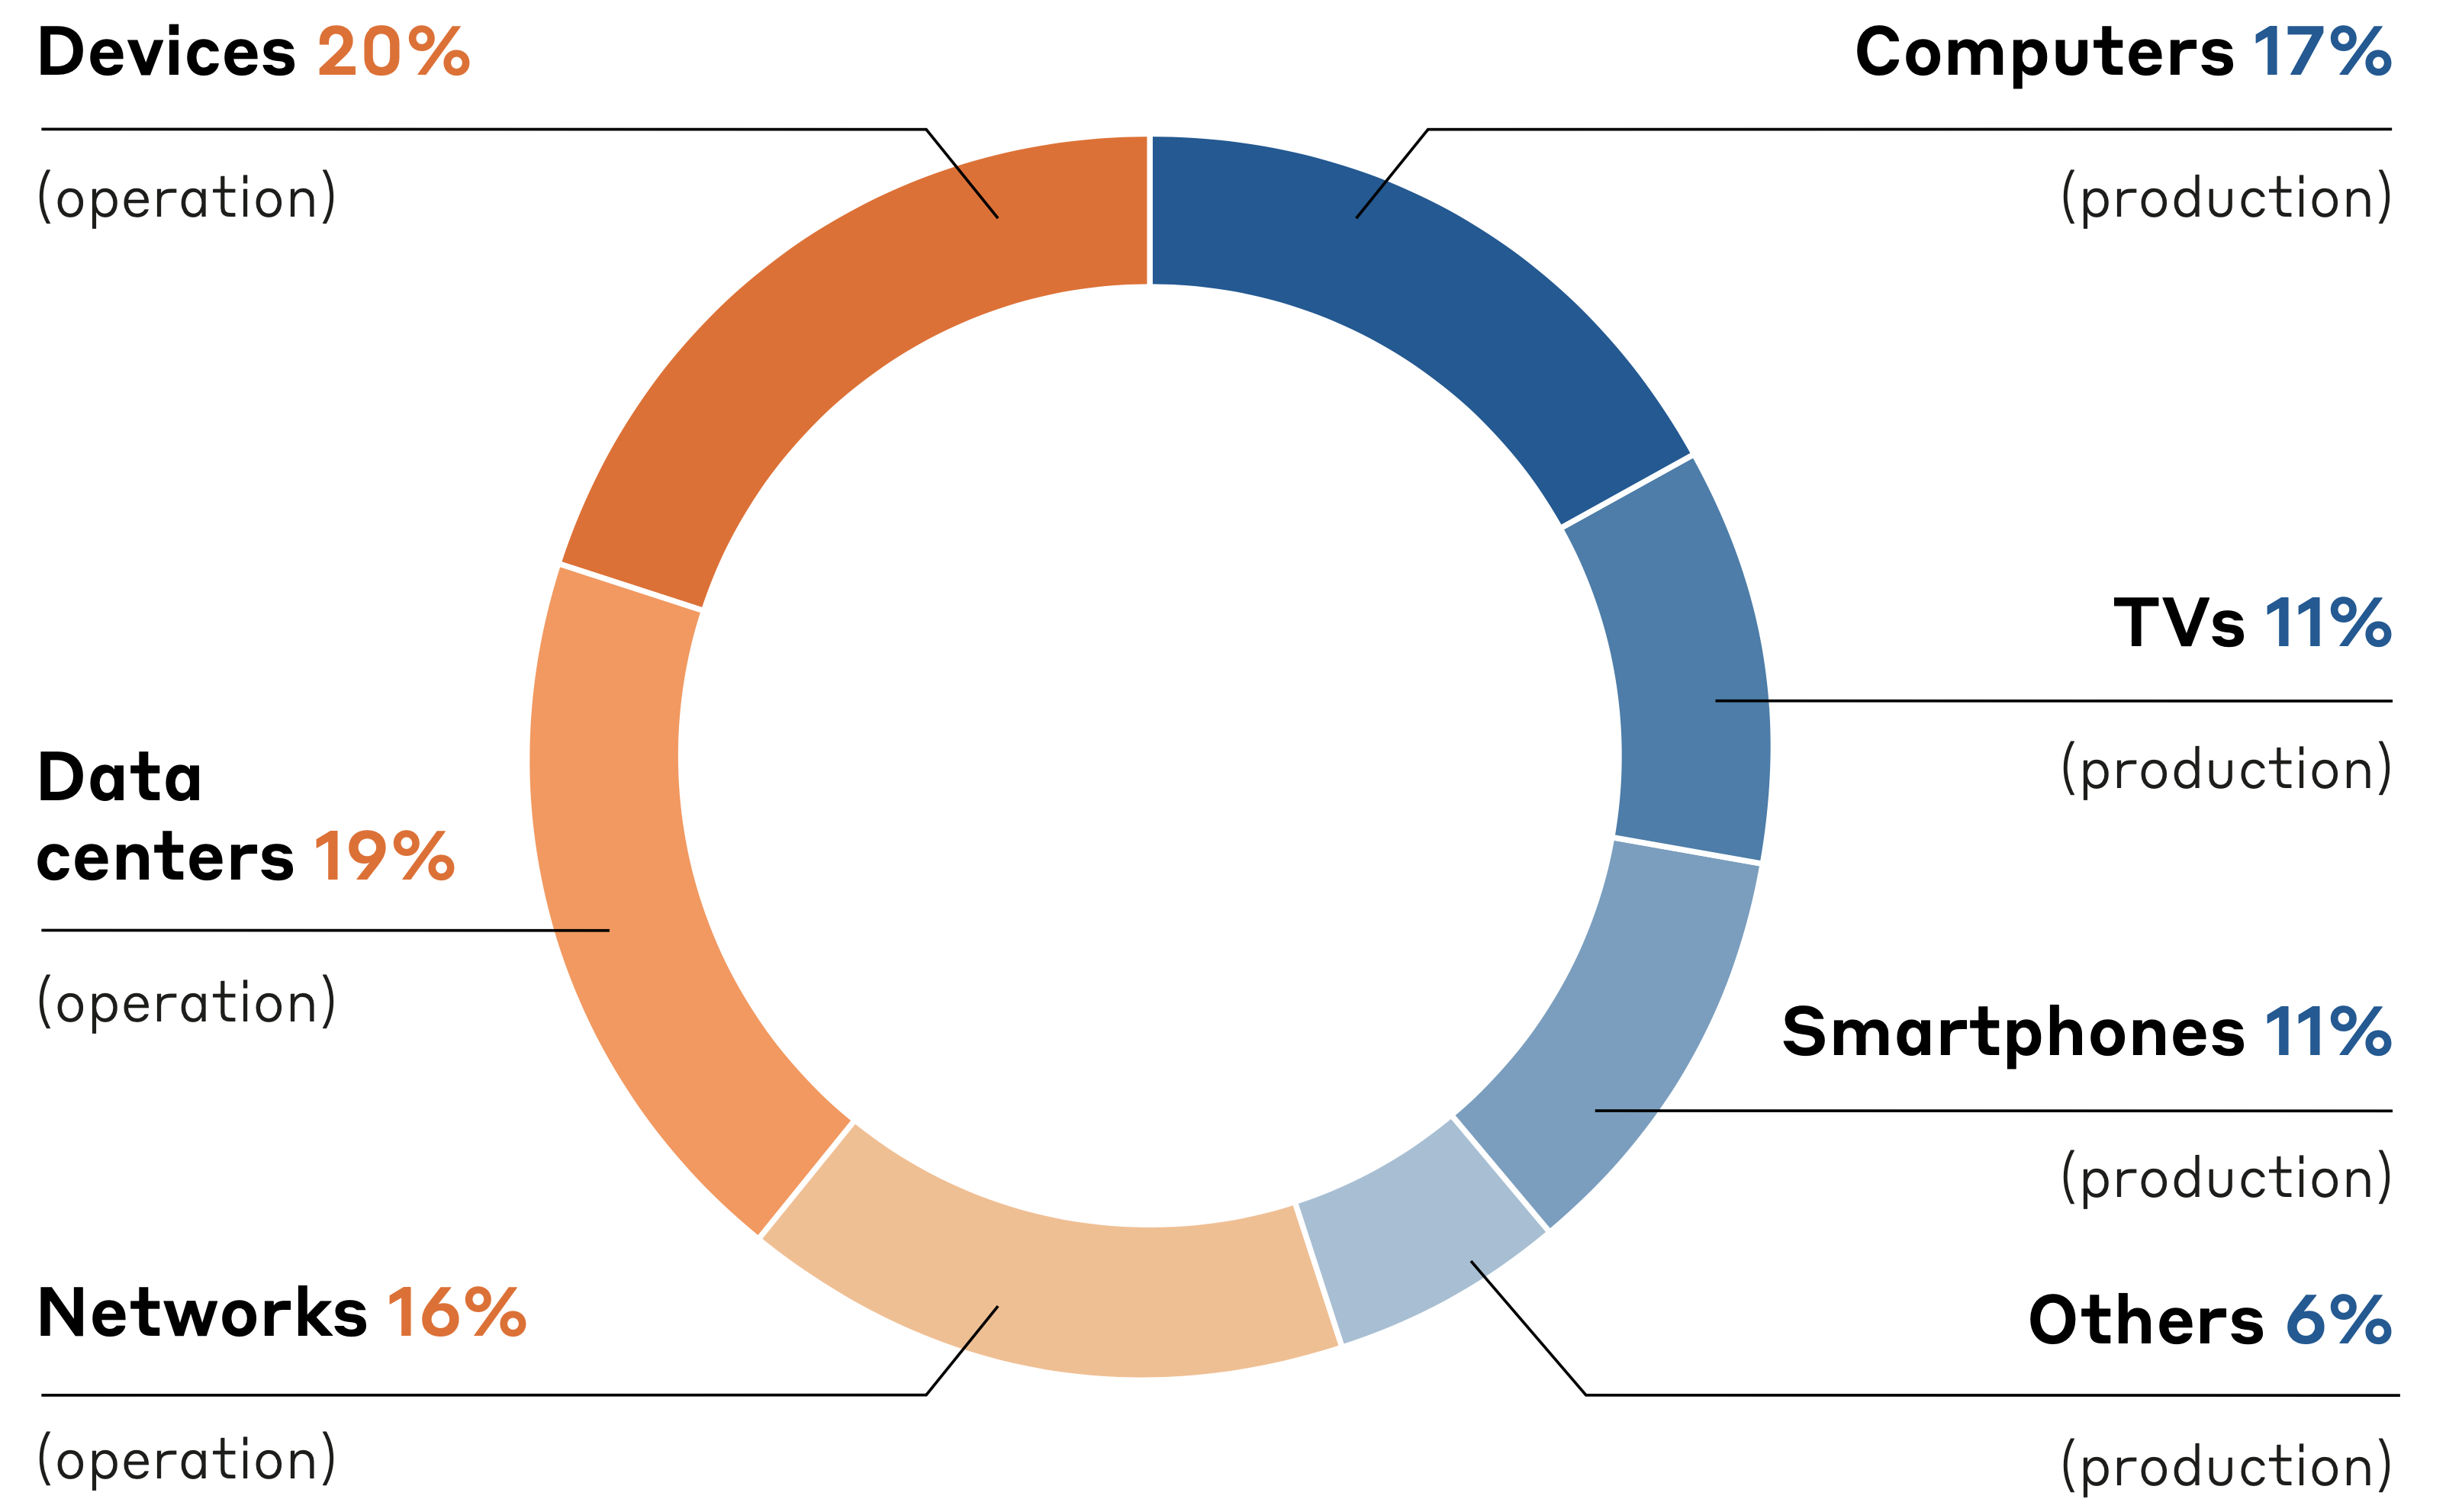
\includegraphics[width=.7\linewidth]{chapters/distribution_of_ict_consumption.png}
    \caption{Final energy consumption of digital technologies by item in 2019(The Shift Project – Forecast Model 2021\cite{shift_2021})}
    \label{fig:distribution_of_ict_consumption}
\end{figure}

Figure~\ref{fig:distribution_of_ict_consumption} shows the distribution of ICT consumption in 2018, where the largest chunk of the energy consumption is due to data usage, aka 63\% of the energy consumed where 22\% of this energy is used by data centers.
Reducing energy consumption means reducing the impact 14\% of the ICT energy consumption has on the environment.

In 2020, the market for data center services was worth 48.9 billion\$.
It is thought that this number will go up to 105.6 billion\$ by 2026~\cite{inshakova2022data}.
This growth is caused mainly by:
\begin{itemize}
    \item shift to remote lifestyle: work, education, and entertainment,
    \item increase in the number of connected devices (IoT),
    \item development of data-hungry technologies such as Machine learning, AI, Big data, and so on,
    \item edge computing and 5G.
\end{itemize}

With this increase in the number of data centers comes an increase in energy consumption, which is a major problem for the environment.
in 2018, data centers consumed around 205 terawatt-hours (TWh)~\cite{schneider2021world}, which is equivalent to the energy consumption of 1\% of the total world's electricity.
This ratio increased up to 1.5 \% in 2020 according to the Journal of Science~\cite{mytton2021data}.
In Figure~\ref{fig:data_centers_power_distribution}, one can see that 40\% of the energy consumed by data centers is used for cooling, while another 40\% is used by the servers themselves.
Therefore, optimizing these two aspects can have a major impact on the energy consumption of data centers.

\begin{figure}[!h]
    \centering
    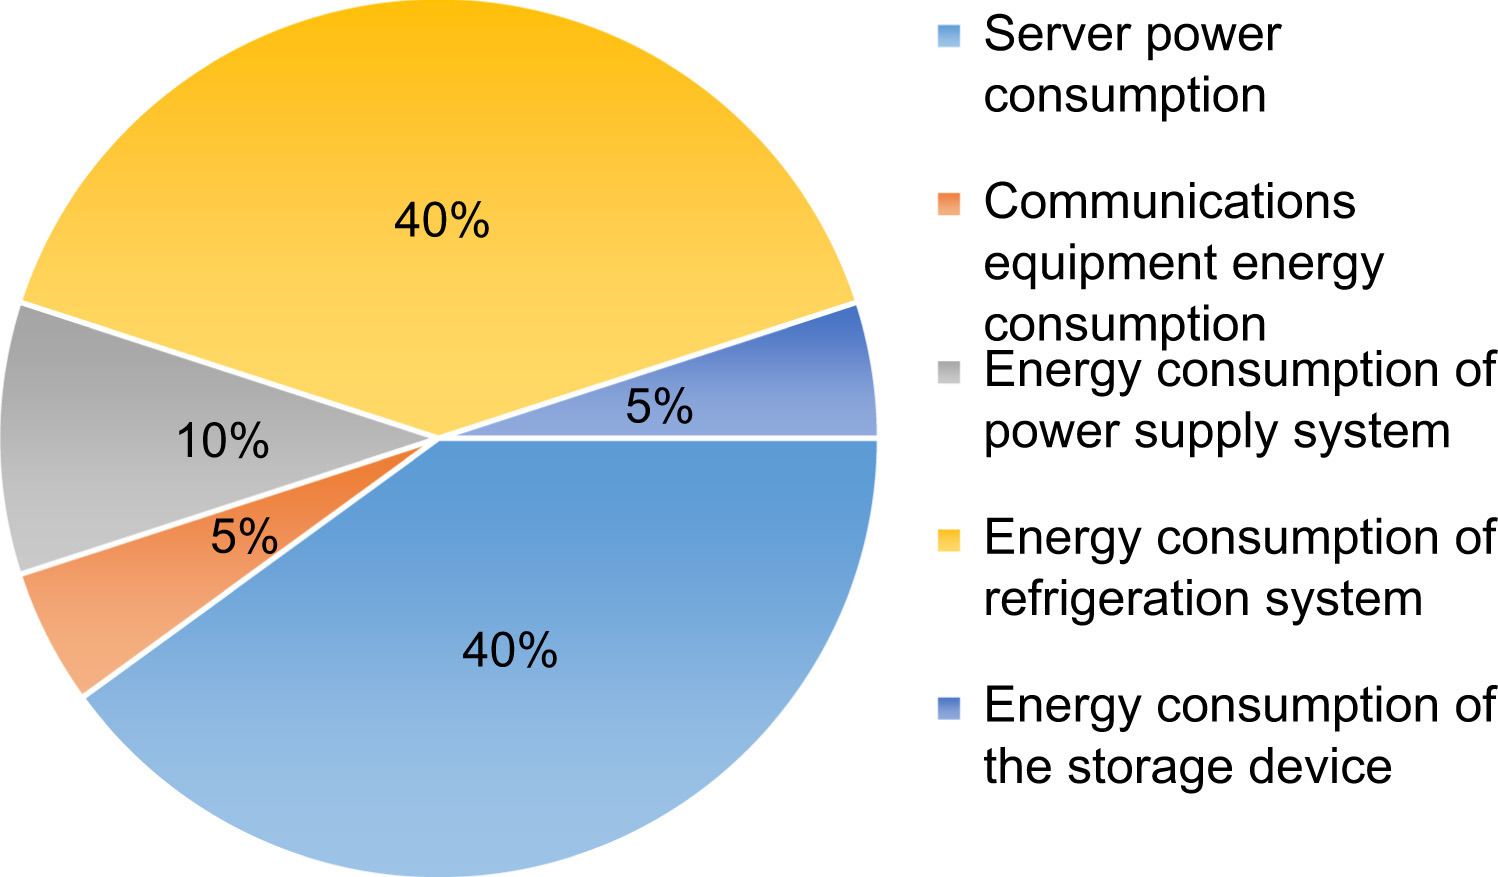
\includegraphics[width=0.6\linewidth]{chapters/data_centers_power_distribution}
    \caption{Distribution of power consumption in a data center~\cite{rong2016optimizing}}
    \label{fig:data_centers_power_distribution}
\end{figure}

Researchers are trying to reduce the energy consumption of data centers through different angles.
Some of the works are focused on the hardware side, such as using new hardware architectures that are more energy-friendly, such as the use of GPUs instead o ARM processors instead of CPUs~\cite{aroca2012towards}.
Others are trying to optimize the cooling system, this can be achieved by using more efficient cooling systems, putting data centers in cold locations or under water~\cite{simon2018project}, or even using the waste heat for other purposes, such as heating buildings~\cite{bouzel2021distributed,cao2021carbon}.

A third approach is to optimize the software, by making software more energy-efficient.
In this thesis, we focus on this approach, and we try to optimize the software by reducing the number of computations that are done by the software.

The best way to do so is to formulate a theory behind the energy consumption of algorithms, such as the complexity and the o notation.
Unfortunately, this is not possible in the current state of the art.
Due to the lack of knowledge about the energy consumption of the algorithms, and the strong correlation between this consumption and the hardware configuration.
Unlike algorithm optimization in the field of performance, which is agnostic toward the platform, the energy consumption of the algorithms is dependent on the execution environment.
Therefore, for the moment, we start by formulating some hypotheses and exploring them using empirical analysis.
Figure~\ref{fig:thesis_position} highlights this thesis's position on the sustainability of ICT\@; while this thesis only addresses a small portion of ICT's energy usage, we feel it is a step in the right direction for additional solutions to mature to preserve humanity.

\begin{figure}[!h]
    \centering
    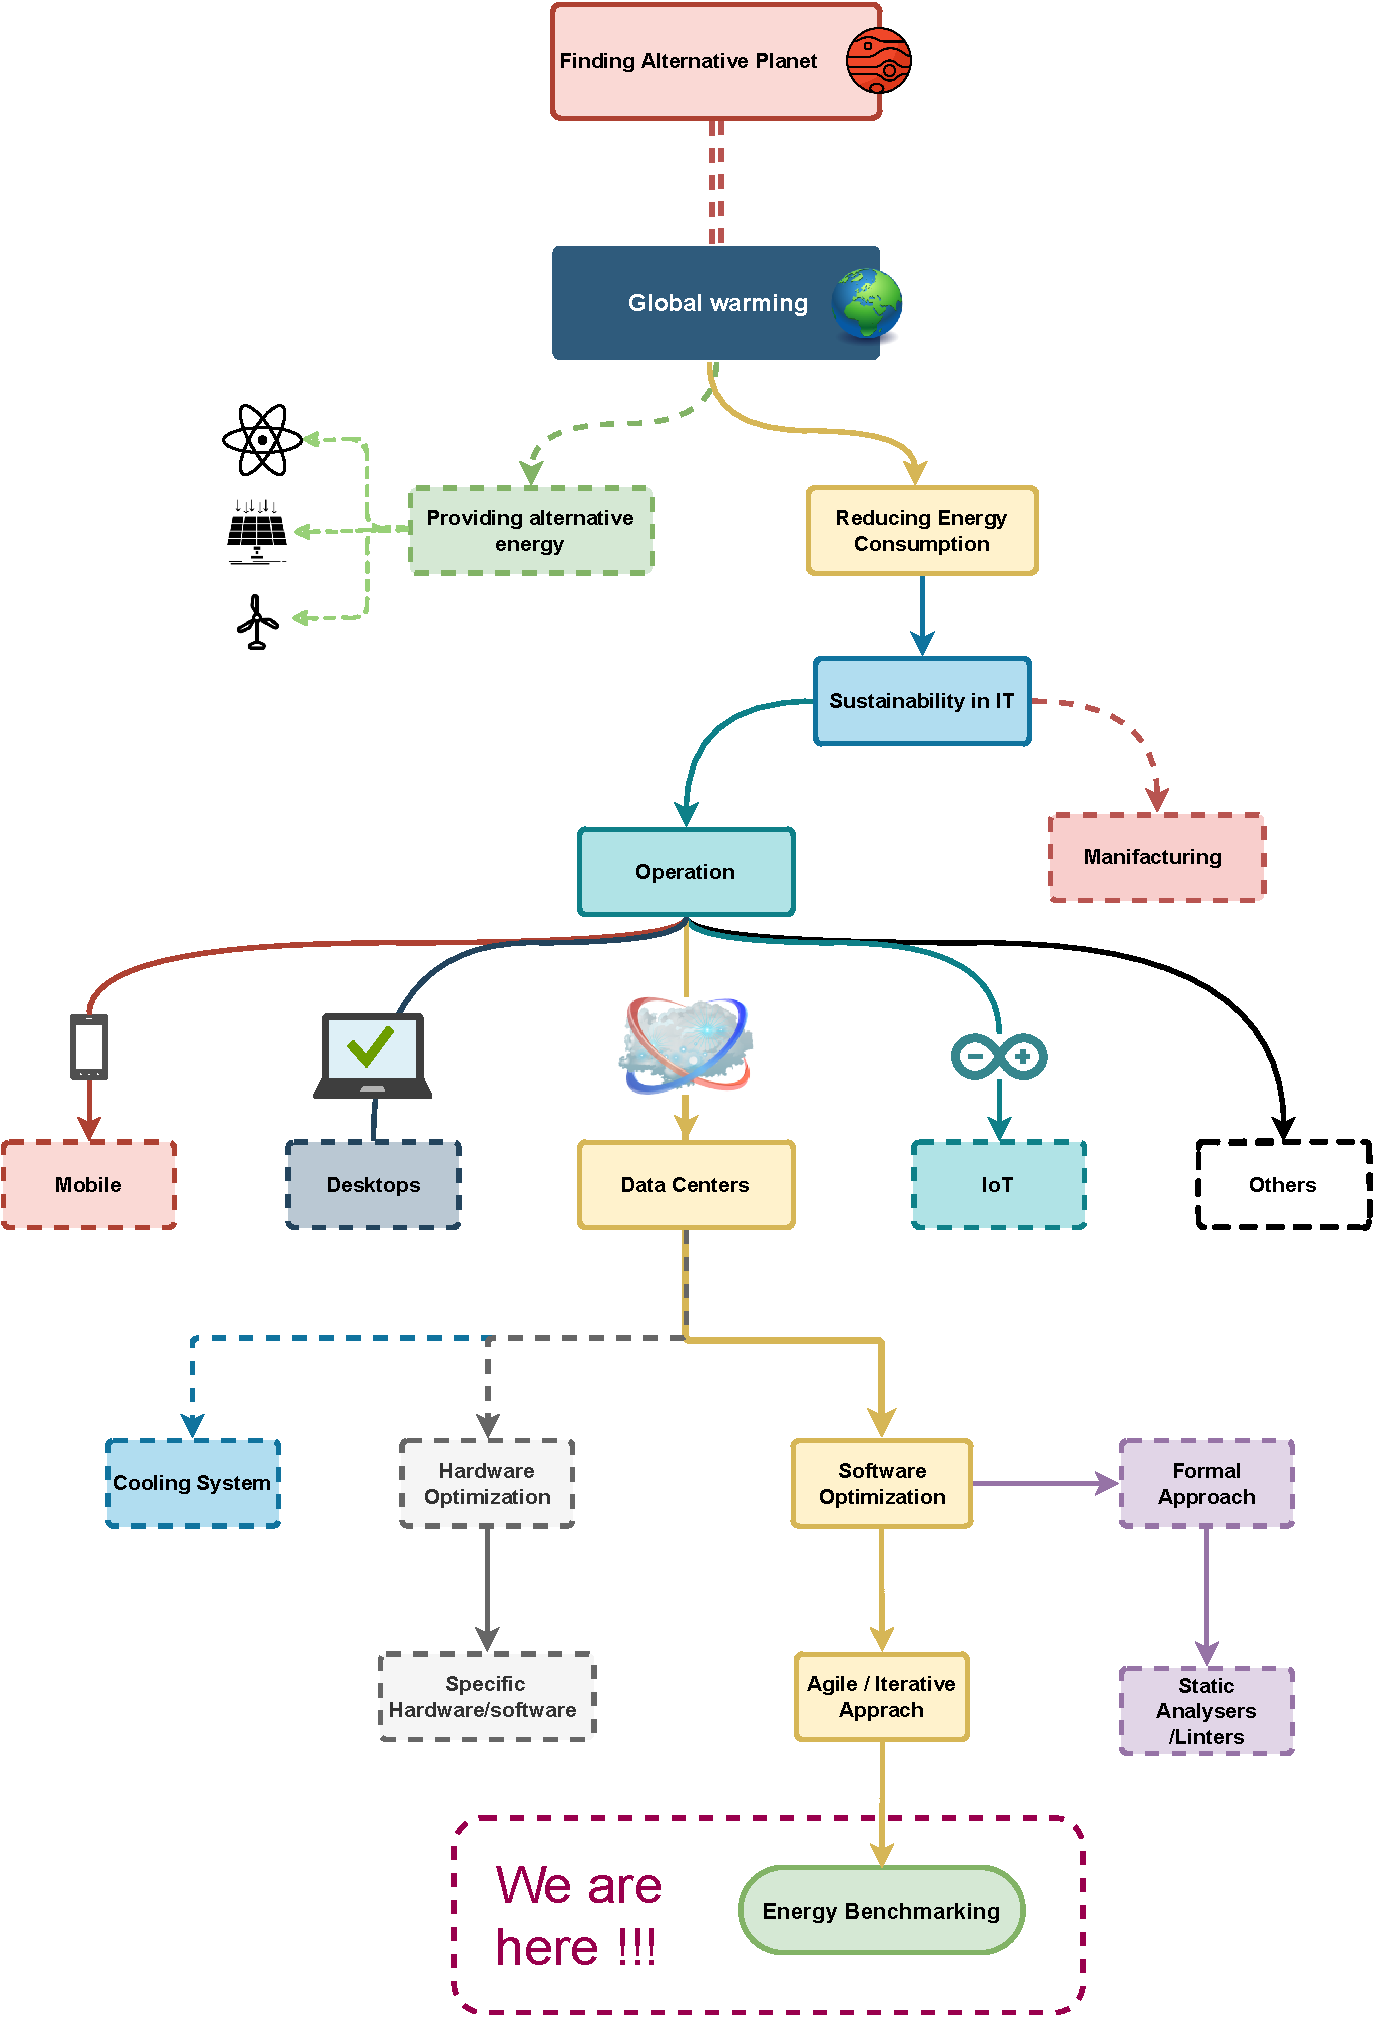
\includegraphics[width=0.7\textwidth,height=\textheight,keepaspectratio]{chapters/thesis_position.pdf}
    \caption{Our position in the IT sustainability research}
    \label{fig:thesis_position}
\end{figure}
\section{Objectives}
The purpose of this thesis is to help developers build more energy-efficient software.
Unfortunately, when it comes to the energy consumption of programs, there is a lack of awareness and knowledge among software developers~\cite{ournani2020reducing,pang2015programmers,pinto2014mining}.
This is mainly due to the lack of tools that can help developers understand the energy consumption of their programs.
Therefore, we aim to provide clear, understandable, and easy-to-use tools and guidelines that can help developers reduce the energy consumption of their programs.

To reduce the energy consumption of software, we can use three strategies.
The first one consists of \emph{reducing energy consumption by reducing the execution time of the program}.
The most intuitive way for developers, as the optimization of software's performance, is a key metric for most programs.
Therefore, in this case, reducing the energy consumption of software becomes a side effect of optimizing the performance of the software.

The second strategy is \emph{optimizing the energy while trying to keep performance}.
In this strategy, we aim to reduce the energy consumption of software without impacting its performance of the software.
This is a more challenging task, as it requires a deeper understanding of the software's energy consumption.
The main focus of this thesis is to provide tools and guidelines that can help developers in this task.

The final strategy consists of \emph{deliberately reducing the performance of the software to reduce its energy consumption}.
The goal of this method is to reduce energy usage by sacrificing execution time.
This strategy is useful while dealing with services since the task has an unlimited execution time.
The second part is to use some. opportunistic schedulers, which will stop the software if it is estimated to spend more energy.
This strategy is discussed first in Chapter~\ref{chapter:porgramming_langauges}, then we continue with this strategy in the perspectives section.

\section{Organization}
\begin{figure}[!h]
    \centering
    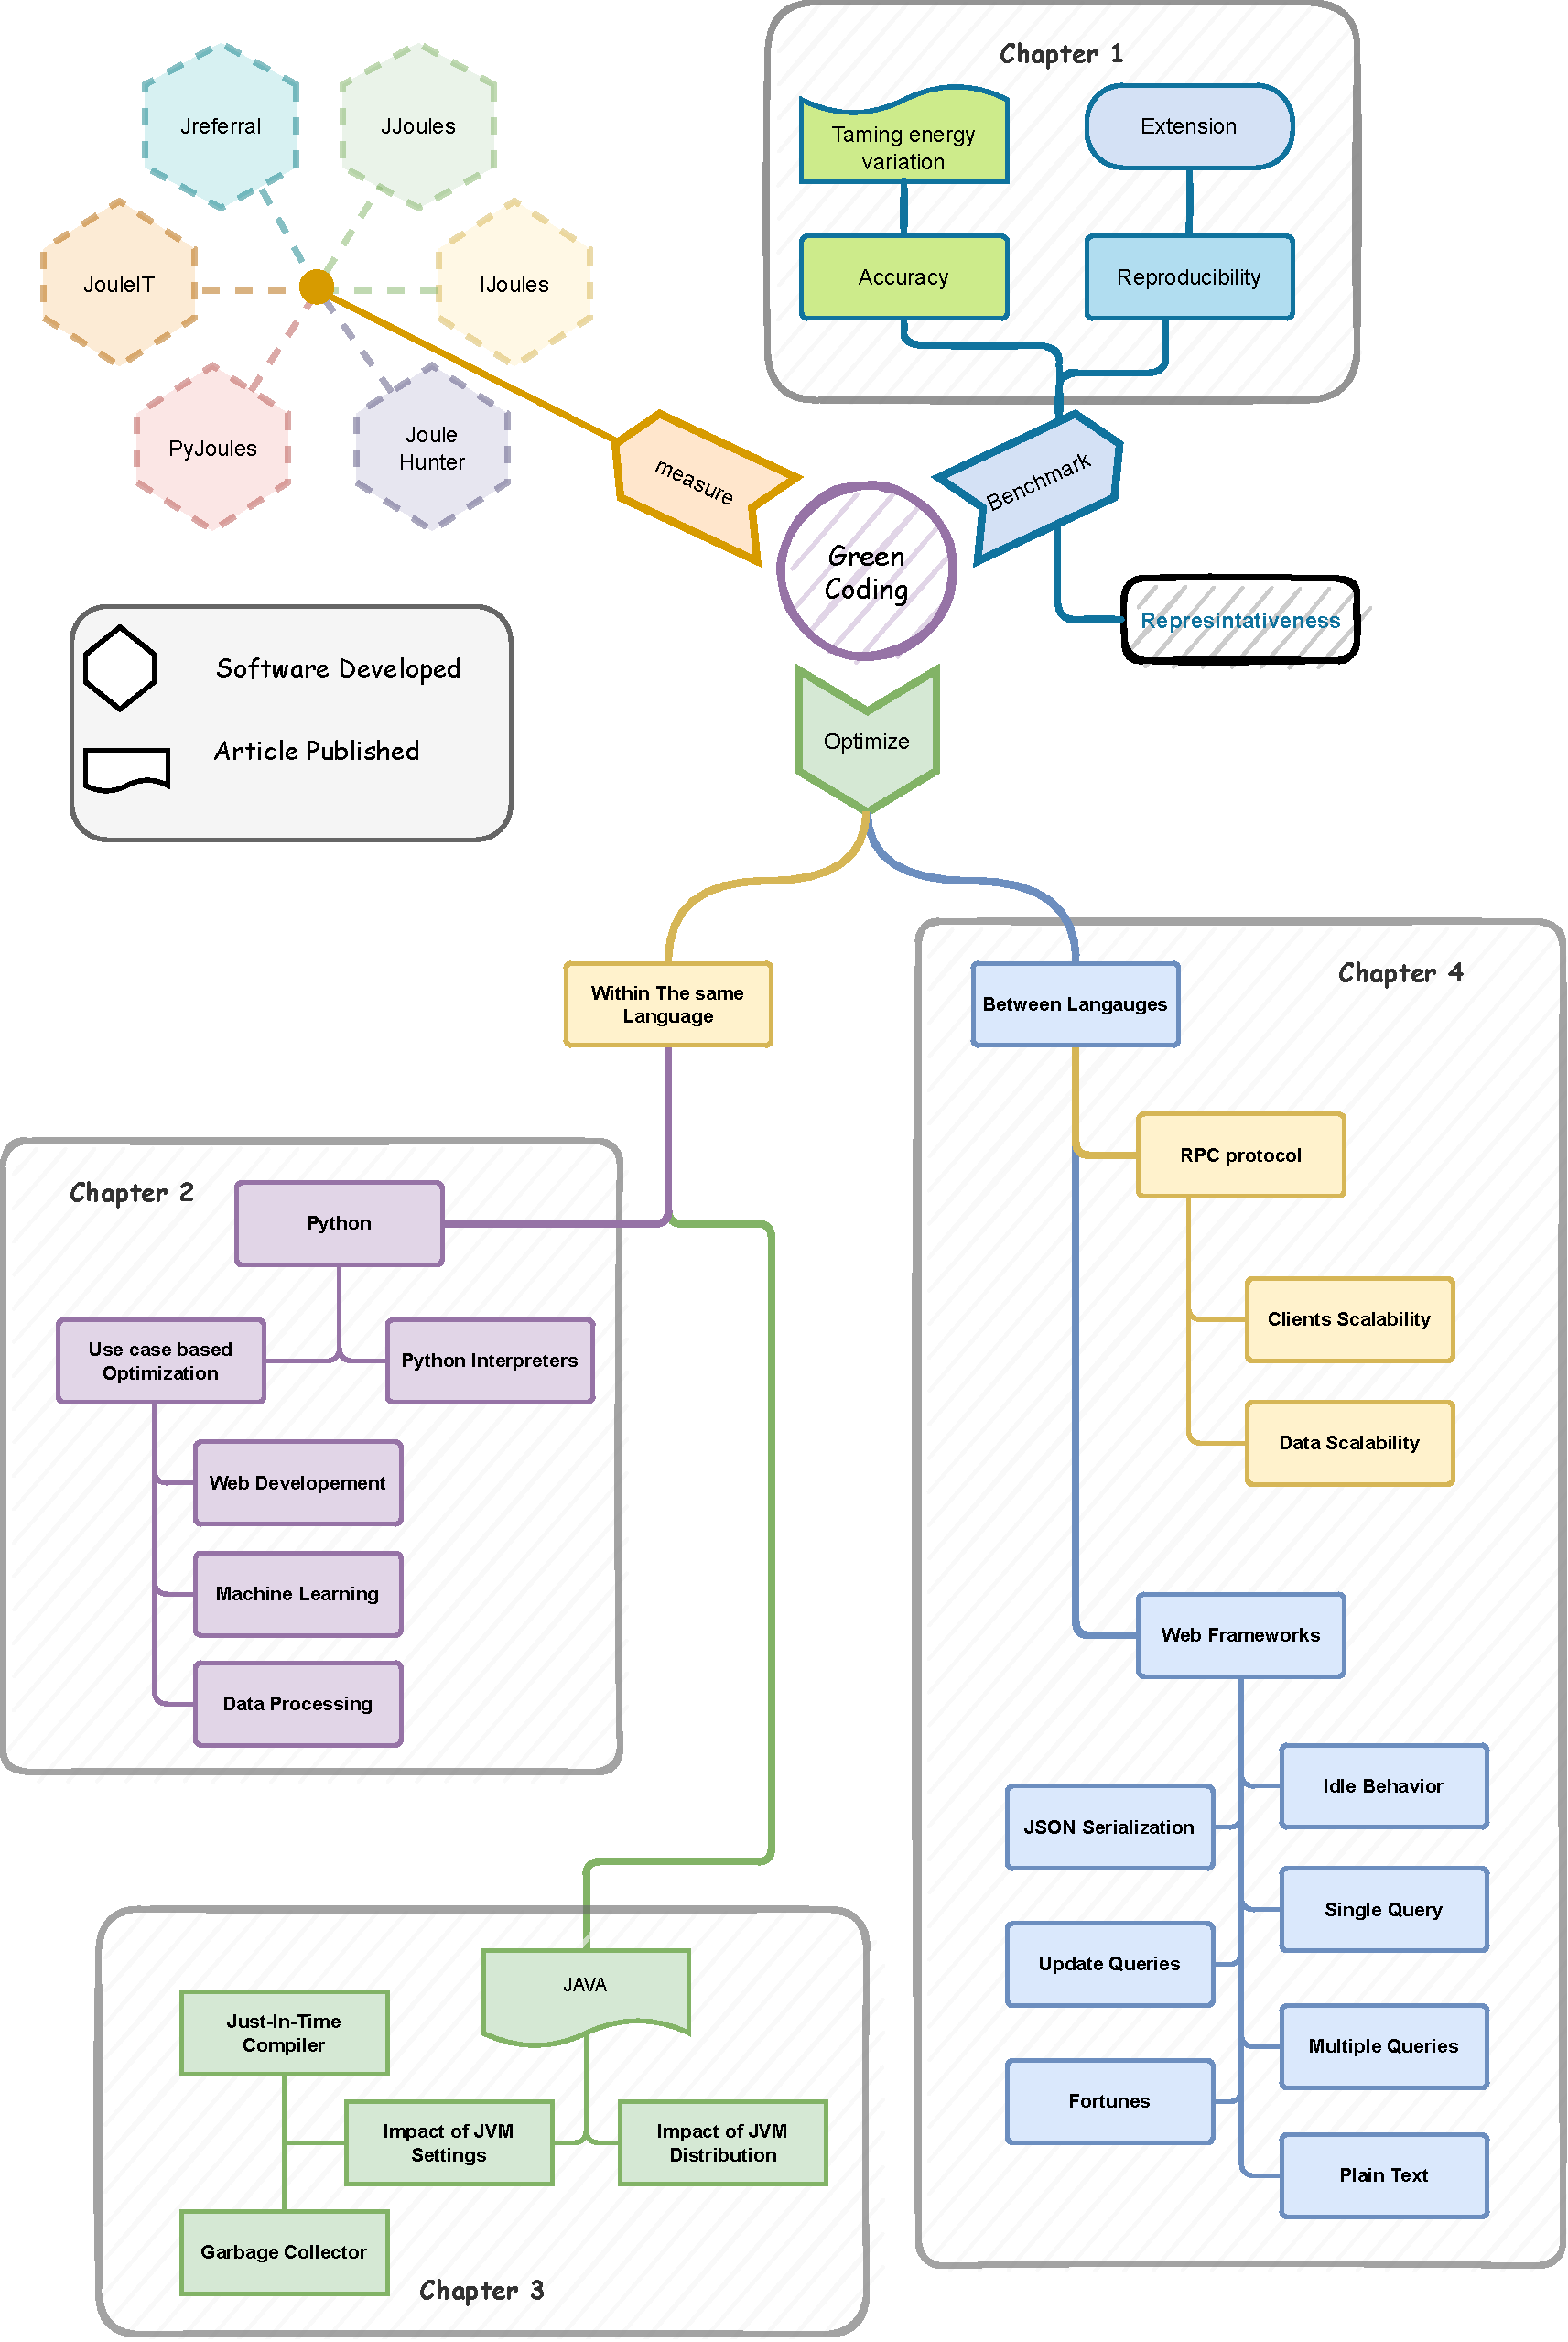
\includegraphics[width=.7\textwidth,height=\textheight,keepaspectratio]{chapters/thesis_contributions.pdf}
    \caption{Contributions reported in this thesis}
    \label{fig:thesis_contributions}
\end{figure}

Figure~\ref{fig:thesis_contributions} summarizes the work completed for this thesis As mentioned in the previous section, our goal is to help developers reduce the energy consumption of their programs during execution.
We use an empirical approach to accomplish this.
As a result, we require some tools to assist us in this task.
To begin, we provide a tool to assist developers in measuring the energy consumption of their programs.
The rest of the manuscript is outlined below.

\begin{itemize}
    \item Chapter~\ref{chapter:literature_review} provides a literature review of the energy consumption of software.
          First, it introduces the challenges that one can encounter when running an empirical study, \emph{reproducibility}, \emph{accuracy}, and \emph{representativeness}, the ways in the state of the art overcome these challenges in the field of computer sciences.
          Then, it narrows down to the energy consumption of software and the challenges that one can encounter when measuring the energy consumption of software.
          In this section, we provide the literature approaches used to measure energy consumption and classify them, compare them and discuss their pros and cons when used for our research. After that, we tackle the challenge of accuracy within the field of energy consumption and discuss how the literature tried to overcome these challenges. Finally, we  present some of the most recent works in the field of software energy consumption optimization;
          % We conclude this chapter by providing a simple method that we will use for the rest of the thesis to optimize the energy consumption of software. \textbf{BMO} : benchmark , measure and optimize.  
    \item Chapter~\ref{chapter:benchmarking} discusses two facets of empirical tests and how we adapt them to energy consumption measurements.
          First, we discuss the reproducibility challenge and how to overcome it with the usage of containers, then we push this approach further by proposing and new protocol to make tests not only reproducible but able to be extended with other features to overcome the rapid pace of software evolution.
          The second part of this chapter discusses the aspect of accuracy when it comes to energy consumption measurements.
          This section demonstrates how energy measurements might differ and produce conflicting results for the same work when run on identical machines or even the same machine.
          Then, it provides some solutions to reduce this energy variation and improve the accuracy of the measurements;
    \item After setting the ground for energy benchmarks in the previous chapter, we discuss the energy consumption of Python, one of the world's most popular programming languages.
          Chapter~\ref{chapter:python} reports on how much python costs in terms of energy consumption compared to other languages.
          Then, it provides some statistics about its popularity and typical use cases and studies the impact of Python on energy consumption in three typical use cases, machine learning, web servers, and data manipulation.
          For each use case, we compare the energy consumption of several approaches and provide guidelines on how to optimize the energy consumption of python programs in these use cases.
          Finally, we provide a non-intrusive way to optimize energy consumption without altering the code of the program.
          We achieve this by using a different implementation of the Python interpreter.
          This not only allows developers to spend less time optimizing their code but also allows them to use it on the legacy code that they cannot modify;
    \item Motivated by the outcomes of the non-intrusive optimization, we follow this strategy on one of the most popular legacy code base applications programming languages, Java.
          In Chapter~\ref{chapter:java}, we try to optimize the Java code, using by changing the default JVM implementation.
          We compare the energy consumption of $12$ benchmarks using $52$ implementation, each benchmark is dedicated to a typical use case.
          After that, we study two of the JVM features, JIT and GC, and show their impact on the energy consumption of the Java code;
    \item In contrast, Chapter~\ref{chapter:porgramming_langauges}  uses the flexibility provided by the micro-services architecture~\cite{dmitry2014micro} to analyze each programming language's energy behavior in light of various web scenarios to optimize the energy use of web services.
          We first examine the effects of the various programming languages when dealing with the \emph{Remote Procedure Call} (RPC) Protocol.
          In this instance, we use two scaling factors: the number of concurrent clients and the size of the requests. Then, we compare $261$ web frameworks, each implementing the same website using seven use cases.
          This analysis aims to look at how each technology uses energy in different kinds of web situations.
    \item Finally, we conclude our work in Chapter~\ref{chapter:conclusion} by summarizing the work done in this thesis and discussing the future work that can be done to further reduce the energy consumption of software.
\end{itemize}

% First, we create a benchmarking protocol that serves researchers and practitioners, experimenting with their approaches and solutions to reduce the energy consumption of programs.
% Then, using this protocol, we analyze and try to optimize the energy consumption of one of the most popular programming languages, Python. We first study python within its most use cases, machine learning, and web Development. Then we try to optimize the energy consumption on the outer side, this can be achieved by targeting the interpreter itself.
% After that, we continue our non-intrusive approach, by targeting the impact of the virtual machine on the JAVA code. This not only helps practitioners improve their software energy without changing their code, but is also beneficial for reducing the energy consumption of the legacy code with almost zero cost.
% Finally, we will shift our focus to other programming languages and compare the energy consumption of different programming languages.
% We consider two main use cases. The RPC protocol, and web servers.

% we have three scenarios, to reduce energy consumption :
% 1. win-win, reducing energy consumption by enhancing the performance: the first one is done by default by most of the developers and performance engineers, which is to optimize the code itself
% 3. win neutral, reducing energy consumption while keeping the same performance: the second one is finding reducing the energy consumption while trying to keep the same performance, which the work of this theses 
% 2. win loose, reducing energy consumption by reducing the performance: optimizing  the energy consumption by sacrificing the performance of the program itself which is what we call  green faas  we will talk about this in the perspective section


% \url{https://www.statista.com/statistics/871513/worldwide-data-created/}
% https://www.iea.org/reports/data-centres-and-data-transmission-networks

% Our work will be presented in the following chapters:
% \begin{enumerate}
%     \item \ref{chapter:literature_review}: Where we discuss the work done on energy consumption and optimization in software engineering
%     \item \ref{chapter: benchmarking}: It will present a set of guidelines and tools to help practitioners measure the energy consumption of their algorithms.
%     \item: it will discuss the behavior of python and the possible ways to tune it in order to reduce the energy consumption
%     \item: will present a study on java programming language and the impact of the JVM choice on the energy consumption
%     \item: we will present the impact of programming languages on the energy consumption of the algorithms especially when it comes to web services.
%     \item: as a perspective, we introduce the impact of parallelism on energy consumption in time-agnostic cases
% \end{enumerate}
% \subsection*{Contributions}


\section{Contributions}
The contributions of this thesis are summarized as follows:
\subsection*{Conferences}
\nobibliography*
\begin{enumerate}
    \item \bibentry{ournani2020taming},
    \item \bibentry{ournani2021evaluating}.
\end{enumerate}

\subsection*{Tools}
% \begin{itemize}
%     \item \textbf{Jouleit} (\url{github.com/powerapi-ng/jouleit}):  \bibentry{Belgaid_JouleHunter_an_2021},
%     \item \bibentry{Belgaid_JRefferal_Which_JVM_2021},
%     \item \bibentry{Belgaid_Jouleit_a_2020},
%           % \item \bibentry{Belgaid_Ijoules_Python_library_2020}
%     \item \bibentry{Belgaid_Pyjoules_Python_library_2019}.
% \end{itemize}
\begin{itemize}
    \item \textbf{Jouleit} (\url{github.com/powerapi-ng/jouleit}): a tool that can be used to monitor energy consumption for any Linux program, this tool was used to compare the energy consumption of different JVMs;
          \\
          \bibentry{Belgaid_Jouleit_a_2020},
    \item \textbf{JRefferal} (\url{github.com/chakib-belgaid/jreferral}): a tool that allows the user to explore the JVM settings and their impact on the energy consumption of a given Java program. This tool was the result of the second article of this thesis;
          \\
          \bibentry{Belgaid_JRefferal_Which_JVM_2021},
    \item \textbf{PyJoules} (\url{pypi.org/project/pyJoules}) is a software toolkit to measure the energy footprint of a host machine along the execution of a piece of Python code. It can measure the energy consumption on the level of script, function, and bloc of code;
          \\
          \bibentry{Belgaid_Pyjoules_Python_library_2019},
    \item \textbf{JouleHunter} (\url{pypi.org/project/joulehunter}): an energy profiler for python applications. It can be used to highlight the functions that consume the most energy in a given Python program. Its main usage is to help developers do an exploratory analysis of their application to scope the functions that should be optimized to be then targeted by PyJoules;
          \\
          \bibentry{Belgaid_JouleHunter_an_2021},
    \item \textbf{GreenBoard} (\url{github.com/chakib-belgaid/greenboard}): a dashboard designed to help developers choose the best stack for their web application. It is based on the results of the third article of the last chapter.
\end{itemize}

% \subsection*{Future Work}
% \begin{itemize}
%     \item Reducing the energy consumption of Python using non-intrusive techniques,
%     \item Empirical analysis on the energy consumption of different web frameworks,
%     \item The impact of programming languages on energy consumption of web services (a case study of RPC protocol),
%     \item How do ORMs affect how much energy is used? A case study of Django and Flask.
% \end{itemize}

% \cleardoublepage

\cleardoublepage

\chapter{State of the Art}
\label{chapter:literature_review}
\import{chapters/literature/}{draft_citations}

% \part{Benchmarking Programming Technologies}

\chapter{Benchmarking Protocol to Measure Software Energy Consumption}\label{chapter:benchmarking}
% \section{Introduction \note{missing} }
This chapter covers ways to overcome empirical analysis challenges in energy consumption studies.
First, we go through the three components of a successful benchmark when performing energy-related experiments.
Section~\ref{sec:benchmarking_reproducibility} focuses on the "reproducibility" challenge---to deliver reproducible experiments without interfering with the energy measurement---while Section~\ref{sec:taming-the-energy-variation} discusses the \emph{accuracy} of software energy consumption.

\import{\currfiledir}{draft}
\import{\currfiledir}{experiment}
\import{\currfiledir}{conclusion}

% However for them to be more representatives we wanted to simulate the production enviromenet.
%% should i add  the thing about green faas ? 
%% same about what we have done with python workers and lazy ? basically just a graph 

% \part{Optimizing Application Runtimes}
\newpage
% \chapter{Optimizating the Software code}
% \label{chapter:optimization}
% \rinclude{chapters/optimization}{java}
% \import{chapters/optimization/java/}{jvms}
% \begin{abstract}
    \vspace{0pt}\noindent\textbf{Background.}
    The \emph{Java Virtual Machine} (JVM) platforms have known multiple evolutions along the last decades to enhance both the performance they exhibit and the features they offer.
    With regards to energy consumption, few studies have investigated the energy consumption of code and data structures.
    Yet, we keep missing an evaluation of the energy efficiency of existing JVM platforms and an identification of the configurations that minimize the energy consumption of software hosted on the JVM.

    \vspace{1pt}\noindent\textbf{Aims.}
    The purpose of this paper is to investigate the variations in energy consumption between different JVM distributions and parameters to help developers configuring the least consuming environment for their Java application.

    \vspace{1pt}\noindent\textbf{Method.}
    We thus assess the energy consumption of some of the most popular and supported JVM platforms using 12 Java benchmarks that explore different performance objectives.
    Moreover, we investigate the impact of the different JVM parameters and configurations on the energy consumption of software.

    \vspace{1pt}\noindent\textbf{Results.}
    Our results show that some JVM platforms can exhibit up to 100\% more energy consumption.
    JVM configurations can also play a substantial role to reduce the energy consumption during the software execution.
    Interestingly, the default configuration of the garbage collector was energy efficient in only 50\% of our experiments.

    \vspace{1pt}\noindent\textbf{Conclusion.}
    Finally, we provide an OSS tool, named \textsf{J-Referral} that recommends an energy-efficient JVM distribution and configuration for any Java application.
\end{abstract}

% \maketitle

\section{Introduction}\label{sec:intro}
Software services are widely deployed to support our daily activities, being mobile or hosted in the cloud.
Yet, beyond this undeniable success, the environmental impact of ICT is raising concerns and calls for solutions to reduce the energy footprint of software services~\cite{the_shift_project_lean_2019}.

Software developers often report that such solutions should come from more energy-efficient hardware components or optimized algorithms~\cite{wang_potential_2018,opaper} but, given the complexity of modern software environments, the composition of software layers makes this sustainability objective particularly challenging.

Given this context, this paper more specifically investigates the impact of one of these layers, the runtime environment and its settings, on the energy consumption of an hosted software service.
More precisely, we aim at revealing the importance of carefully selecting and configuring the \emph{Java Virtual Machine} (JVM) to reduce the energy consumption of any software service built from any language compatible with the Java ecosystem (Java, Kotlin, Scala, Groovy, Clojure, Jython, etc.).

The empirical study we conduct in this paper reports on the energy footprint of several versions of popular JVM distributions that are freely available for download.
Beyond the choice of an appropriate runtime and its most energy-efficient version, we also consider the impact of exposed JVM settings to maximize the energy savings for a given software service.
The observations of this study aim to quantify the role played by internal JVM mechanisms, like the \emph{Just in Time} (JIT) compiler and the \emph{Garbage Collector} (GC), in the reduction of the energy consumption of hosted applications.
More formally, we formulate the following research questions:
\begin{compactenum}[\indent\bf RQ\,1:]
    \item \emph{What is the impact of existing JVM distributions on the energy consumption of Java-based software services?}
    \item \emph{What are the relevant JVM settings that can reduce the energy consumption of a given software service?}
\end{compactenum}

By answering these questions, we envision supporting application developers and administrators in the configuration of their production environment by substantially reducing the energy consumption of hosted services at large.
We also hope that our results will encourage the JVM developers to keep investing in the integration of further optimizations that can benefit a large population of software services.
This paper comes with a set of contributions that can be summarized as:
\begin{compactenum}[\indent\em (a)]
    \item Reporting on the energy-efficiency of a large panel of JVM when running acknowledged benchmarks,
    \item Identifying and assessing the key JVM settings that can influence the energy consumption of a software service,
    \item Sharing guidelines and prerequisites that will help in configuring the most energy-efficiency environment before deployment,
    \item Providing a JVM benchmarking environment to evaluate the energy-efficiency of upcoming JVM distributions and their settings,
    \item Delivering an open-source tool, named \textsf{J-Referral}, to recommend the most energy efficient JVM distribution among 85 JVMs/versions and hundreds of configurations for Java applications.
\end{compactenum}

The remainder of this paper is organized as follows.
\Cref{sec:meth} introduces the experimental protocol and methodology (hardware, projects, tools, and methodology) we adopted in this study.
\Cref{sec:exp} analyzes the results of our experiments on the energy consumption of the different JVM configurations.
\Cref{sec:rw} discusses the related works to reduce the energy consumption of Java-based Software Services.
%Finally, \Cref{sec:threats,sec:ccl} cover the validity threats and our conclusions, respectively.
Finally, \Cref{sec:ccl} covers our conclusions.

% Energy efficiency is a major concern in software engineering.
% Indeed, the huge leap in technology with all the mobile devices, IoT, cloud computing, etc. raised serious questions about the way energy is consumed. 
% In most domains, we often aim to reduce the consumption of the electronic devices/parts while improving.
% In computer science, many researches were interested in the EC optimization.
% Some of the works focused on reducing the EC at the hardware or the OS level, others by optimizing software's source codes consumption.
% In this paper, we focus on the JVM based languages, especially Java.
% Many works wave been conducted to reduce the Java and JVM based software energy consumption \cite{}.
% These works focused on many aspects of the source code such as the data collections, control structures,  code refactoring ,etc.
% Other works focused on aspects that are closer to the JVM execution such as bytecode energetic cost analysis \cite{brownlee_search_based_2017,grass_energy_2006} and the consumption that can exhibit the same source code written in many languages that can use the JVM \cite{pereira_energy_2017}.
% However, even with the increasing concern about software energetic efficiency, we still lack some basic knowloedge on how to parameter and configure the execution environment do the software can run in ideal conditions and thus consume less energy.
% Hence, our study aims at constituting a set of knowledge on the basic choices and configurations that one can apply on a JVM to reduce the energy consumption.
% Concretely, we benchmark different JVM plateforms from different providers, along with different configurations and parameters of threads management, Just In Time compiler (JIT) and Garbage Collector (GC).
% The puropose of this study is to check if some configurations can play a substantial role in reducing software energy consumption.
% In particular, if the use the default JVM with a default configuration can be a reason for energy consumption increase and how often can that be. 
% This study, therefore, aims to answer the following research questions:
% \begin{description}
% 	\item[\textbf{RQ\,1}:] What is the impact that can a JVM exhibit on the energy consumption of the running software?
% 	\item[\textbf{RQ\,2}:] How can one properly configure his JMV to to reduce software energy consumption?
% \end{description}

\section{The Java Virtual Machine}\label{sec:background}
Java was originally developed by James Gosling at Sun~Microsystems and released in 1995, before being acquired by Oracle in 2010.
One key design goal of Java is portability, which means that Java applications must run similarly on any combination of hardware and operating system with adequate runtime support.
This is achieved by compiling the Java language code to an intermediate representation, called Java \emph{bytecode}, instead of machine code.
Java bytecode instructions are analogous to machine code, but executed by a \emph{Java Virtual Machine} (JVM), which is specific to the host machine.
For example, Oracle keeps offering the \textsc{HotSpot}\,JVM, while the official reference implementation is now the \textsc{OpenJDK}\,JVM---a free and open-source software used by most developers.

Programs written in Java have a reputation for being slower and requiring more memory than those written in C++, but \emph{Just-in-Time} (JIT) compilation, embedded in the JVM, delivers a boost of performance by opportunistically compiling bytecode to machine code at runtime.
The JIT combines two compilers, C1 and C2 (also known as Client \& Server\,VM), which are triggered based on the activity of the hosted application.
Additionally, Java uses an automatic \emph{garbage collector} (GC) to manage memory in the object lifecycle and recovering the memory once objects are no longer in use.
Each JVM usually includes multiple GC, each designed to satisfy different requirements.

By default, \textsc{HotSpot} uses both C1 and C2 as tiered compilers,\footnote{\url{http://www.ittc.ku.edu/~kulkarni/teaching/EECS768/19-Spring/Idhaya_Elango_JIT.pdf}} and the \emph{Garbage-First} (G1) GC with a maximum number of GC threads limited by available CPU resources and heap size, whose initial size is set $1/64^{th}$ of physical memory and maximum size may reach up to $1/4^{th}$ of physical memory.\footnote{https://docs.oracle.com/en/java/javase/15/gctuning/ergonomics.html}

%\begin{figure}%[ht]
%	\centering
%	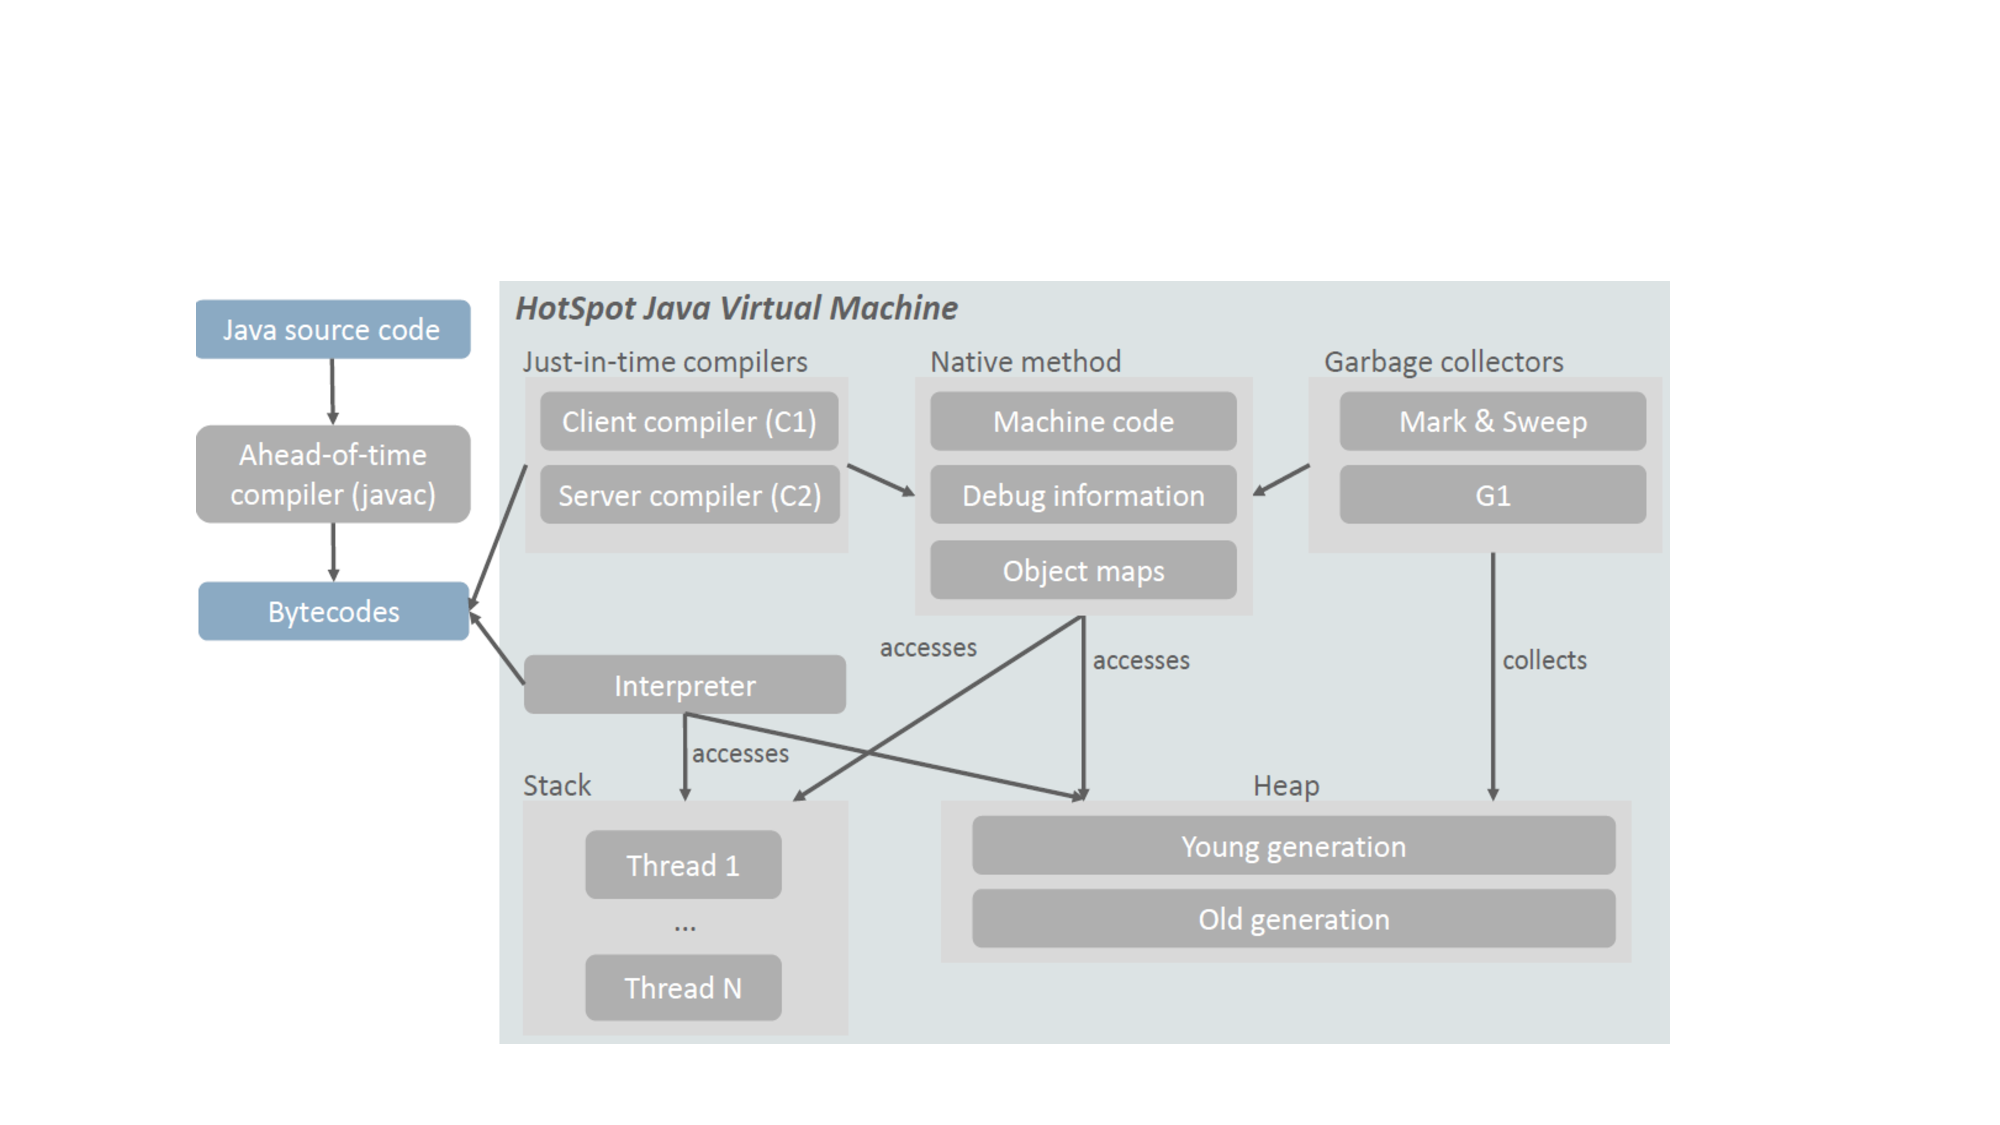
\includegraphics[width=\linewidth]{imgs/hotspot-jvm.pdf}
%	\caption{Overview of the HotSpot JVM key components.}
%	\label{fig:hotspot}
%\end{figure}

At the time of writing this paper, the latest JVM version is Java\,15, released in September~2020, while Java\,11 is the current \emph{Long-Term Support} (LTS) version.
As Java\,9, 10, 12, and 13 are no longer supported, Oracle advises developers to immediately transition to the latest version (currently Java\,15), or an LTS release.

Beyond \textsc{HotSpot}, one can observe that the initial JVM design leads to numerous initiatives to improve the performances of Java applications, including new hotswapping strategies---with the \emph{Dynamic Code Evolution Virtual Machine} (DCE\,VM)~\cite{DBLP:journals/scp/WurthingerWS13}---or alternative JIT---with \textsc{GraalVM}.\footnote{\url{https://www.graalvm.org}}
This also includes alternative implementations, like IBM\,J9 JVM, which is currently distributed as part of the Eclipse foundation, and known as \textsc{J9}.\footnote{https://www.eclipse.org/openj9}
Given the wide diversity of distributions and related settings, this paper aims to study the impact of the features implemented by available JVM distributions on the energy consumption of the hosted Java software services.

\section{Experimental Protocol}\label{sec:meth}
To investigate the effect that could have the JVM distribution choice and/or parameters on software energy consumption, we conducted a wide set of experiments on a cluster of machines and using several established Java benchmarks and JVM configurations.

\vspace{6pt}
\noindent\textbf{Hardware Settings.}
To report on reproducible measurements, we used the cluster \textsf{Dahu} of the G5K platform~\cite{grid5000} for most of our experiments.
This cluster is composed of $32$ identical compute nodes, which are equipped with $2$ Intel Xeon\,Gold\,6130 and 192\,GB of RAM.
Our experimental protocol enforces that the software under test is the only process executed on the node configured with a very minimal Linux Debian\,9 (4.9.0 kernel version).
The minimal OS configuration ensures that only mandatory services and daemons are kept active to conduct robust experiments and reduce the factors that can affect the energy consumption measurements during our experiments~\cite{opaper}.

\vspace{6pt}
\noindent\textbf{Energy Measurements.}
We used Intel\,RAPL as a physical power~meter to analyze the energy consumption of the CPU package and the DRAM.
RAPL is one of the most accurate tools to report on the global energy consumption of a processor~\cite{Khan:2018:RAE:3199681.3177754,10.1145/2989081.2989088}.
We note that, due to CPU energy consumption variations issues~\cite{opaper}, we used the same node for all our experiments.
% In other words, we used the same node to ran all the JVM from the different providers and with numerous configurations for each single benchmark application.
Moreover, we tried to be very careful, while running our experiments, not to fall in most common benchmarking "crimes"~\cite{crimes}.
Every single experiment, therefore, reports on energy metrics obtained from at least $20$ executions of $50$ iterations per benchmark.
All of our experiments are available for use/reproducibility from our anonymous repository.\footnote{\url{https://anonymous.4open.science/r/jvm-comparaison-213E/Readme.md}}

\vspace{6pt}
\noindent\textbf{Java Virtual Machines.}
We considered a set of $52$ JVM distributions taken from $8$ different providers/packagers mostly obtained from \textsf{SDKMAN!},\footnote{\url{https://sdkman.io/}} as listed in \Cref{tab:JVM}.
Depending on providers, either all the versions, majors, or LTS are made available by \textsf{SDKMAN!}.

\begin{table}
    \centering
    \caption{List of selected JVM distributions.}
    \label{tab:JVM}
    \resizebox{\linewidth}{!}{
        \begin{tabular}{|c|c|c|l|}
            \hline
            \textbf{Distribution} & \textbf{Provider}       & \textbf{Support} & \textbf{Selected versions}                                               \\
            \hline
            \hline
            \textsc{HotSpot}      & \textbf{Adopt\,OpenJDK} & {\sc All}        & 8.0.275, 11.0.9, 12.0.2, 13.0.2, 14.0.2, 15.0.1                          \\
            \hline
            \textsc{HotSpot}      & \textbf{Oracle}         & {\sc All}        & 8.0.265, 9.0.4, 10.0.2, 11.0.2, 12.0.2, 13.0.2, 14.0.2, 15.0.1, 16.ea.24 \\
            \hline
            \textsc{Zulu}         & \textbf{Azul\,Systems}  & {\sc All}        & 8.0.272, 9.0.7, 10.0.2, 11.0.9, 12.0.2, 13.0.5, 14.0.2, 15.0.1           \\
            \hline
            \textsc{SapMachine}   & \textbf{SAP}            & {\sc All}        & 11.0.9, 12.0.2, 13.0.2, 14.0.2, 15.0.1                                   \\
            \hline
            \textsc{Librca}       & \textbf{BellSoft}       & {\sc All}        & 8.0.275, 11.0.9, 12.0.2, 13.0.2, 14.0.2, 15.0.1                          \\
            \hline
            \textsc{Corretto}     & \textbf{Amazon}         & {\sc Mjr}        & 8.0.275, 11.0.9, 15.0.1                                                  \\
            \hline
            \textsc{HotSpot}      & \textbf{Trava\,OpenJDK} & LTS              & 8.0.232, 11.0.9                                                          \\
            \hline
            \textsc{Dragonwell}   & \textbf{Alibaba}        & LTS              & 8.0.272, 11.0.8                                                          \\
            \hline
            \textsc{OpenJ9}       & \textbf{Eclipse}        & {\sc All}        & 8.0.275, 11.0.9, 12.0.2, 13.0.2, 14.0.2, 15.0.1                          \\
            \hline
            \textsc{GraalVM}      & \textbf{Oracle}         & LTS              & 19.3.4.r8, 19.3.4.r11, 20.2.0.r8, 20.2.0.r11                             \\
            \hline
            \textsc{Mandrel}      & \textbf{Redhat}         & LTS              & 20.2.0.0                                                                 \\
            \hline
        \end{tabular}
    }
\end{table}

\begin{table*}[t]
    \centering
    \caption{List of selected open-source Java benchmarks taken from \textsc{Dacapo} and \textsc{Renaissance}.}
    \label{tab:benchmarks}
    \resizebox{\linewidth}{!}{
        \begin{tabular}{|p{0.1\linewidth}|p{0.6\linewidth}|p{0.3\linewidth}|}
            \hline
            \textbf{Benchmark}    & {\bf Description}                                                                                                    & \textbf{Focus}                             \\
            \hline
            \hline
            \textsf{ALS}          & Factorize a matrix using the alternating least square algorithm on spark                                             & Data-parallel, compute-bound               \\
            \hline
            \textsf{Avrora}       & Simulates and analyses for AVR microcontrollers                                                                      & Fine-grained multi-threading, events queue \\
            \hline
            \textsf{Dotty}        & Uses the dotty Scala compiler to compile a Scala codebase                                                            & Data structure, synchronization            \\
            \hline
            \textsf{Fj-Kmeans}    & Runs K-means algorithm using a fork-join framework                                                                   & Concurrent data structure, task parallel   \\
            \hline
            \textsf{H2}           & Simulates an SQL database by executing a TPC-C like benchmark written by Apache                                      & Query processing, transactions             \\
            \hline
            \textsf{Lusearch}     & Searches keywords over a corpus of data comprising the works of Shakespeare and the King James bible                 & Externally multi-threaded                  \\
            \hline
            \textsf{Neo4j}        & Runs analytical queries and transactions on the Neo4j database                                                       & Query Processing, Transactions             \\
            \hline
            \textsf{Philosophers} & Solves dining philosophers problem                                                                                   & Atomic, guarded blocks                     \\
            \hline
            \textsf{PMD}          & Analyzes a list of Java classes for a range of source code problems                                                  & Internally multi-threaded                  \\
            \hline
            \textsf{Reactors}     & Runs a set of message-passing workloads based on the reactors framework                                              & Message-passing, critical-sections         \\
            \hline
            \textsf{Scrabble}     & Solves a scrabble puzzle using Java streams                                                                          & Data-parallel, memory-bound                \\
            \hline
            \textsf{Sunflow}      & Renders a classic Cornell box; a simple scene comprising two teapots and two glass spheres within an illuminated box & Compute-bound                              \\
            \hline
        \end{tabular}
    }
\end{table*}

\vspace{6pt}
\noindent\textbf{Java Benchmarks.}
We ran our experiments across $12$ Java benchmarks we picked from \textsf{OpenBenchmarking.org}.\footnote{\url{https://openbenchmarking.org}}
This includes $5$ acknowledged benchmarks from the \textsc{Dacapo} benchmark suite v.\,9.12~\cite{DaCapo:paper}, namely \textsf{Avrora}, \textsf{H2}, \textsf{Lusearch}, \textsf{Sunflow} and \textsf{PMD}, that have been widely used in previous studies and proven to be accurate for memory management and computer architecture communities~\cite{DBLP:conf/wosp/LengauerBMW17,DBLP:conf/oopsla/KaliberaMJV12}.
It consists of open-source and real-world applications with non-trivial memory loads.
% 
Then, we also considered $7$ additional benchmarks from the \textsc{Renaissance} benchmark suite~\cite{renaissance,DBLP:conf/pldi/ProkopecRLD0SBZ19}, namely \textsf{ALS}, \textsf{Dotty}, \textsf{Fj-kmeans}, \textsf{Neo4j}, \textsf{Philosophers}, \textsf{Reaction} and \textsf{Scrabble}, which offers a diversified set of benchmarks aimed at testing JIT, GC, profilers, analyzers, and other tools.
The benchmarks we picked from both suites exercise a broad range of programming paradigms, including concurrent, parallel, functional, and object-oriented programming.
\Cref{tab:benchmarks} summarizes the selected benchmarks with a short description.


\section{Experiments \& Results}\label{sec:exp}
\subsection{Energy Impact of JVM Distributions}
\noindent\textbf{Job-oriented applications.}
To answer our first research question, we executed $62,400$ experiments by combining the $52$ JVM distributions with the $12$ Java benchmarks, thus reasoning on $100$ energy samples acquired for each of these combinations.
\Cref{fig:JVMs} first depicts the accumulated energy consumption of the $12$ Java benchmarks per JVM distribution and major versions (or LTS when unavailable).
Concretely, We measure the energy consumption of each of the benchmarks and compute the ratio of energy consumption compared to \textsc{HotSpot-8}, which we consider as the baseline in this experiment.
Then, we sum the ratios of the $12$ benchmarks and depict them as percentages in \Cref{fig:JVMs}.

\begin{figure*}%[ht]
    \centering
    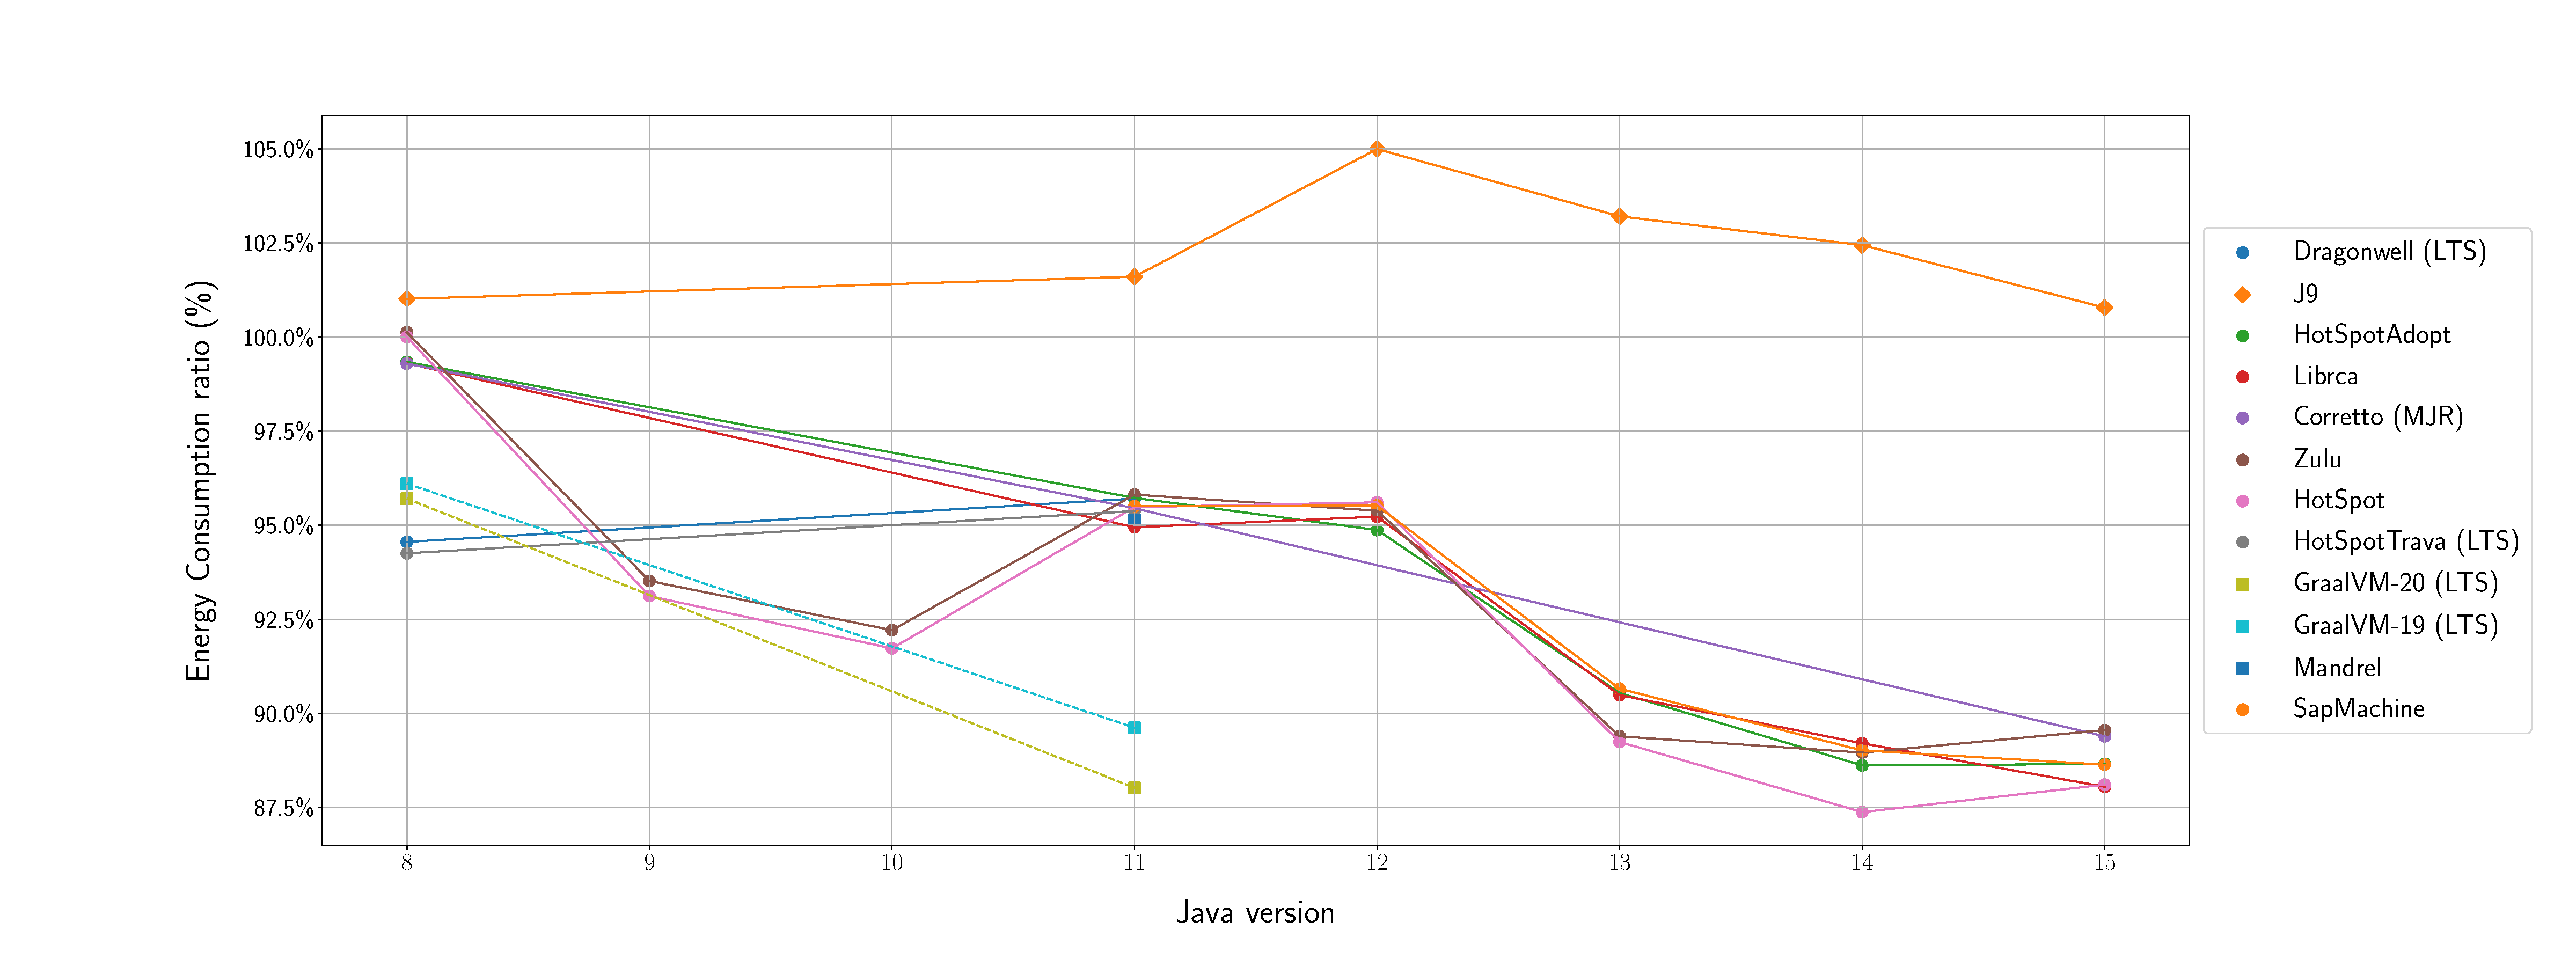
\includegraphics[width=\linewidth]{imgs/alljvms_chetemi8_baseon8.pdf}
    \caption{Energy consumption evolution of selected JVM distributions along versions.}
    \label{fig:JVMs}
\end{figure*}

One can observe that, along with time and versions, the energy efficiency of JVM distributions tends to improve (10\% savings), thus demonstrating the benefits of optimizations delivered by the communities.
Yet, one can also observe that energy consumption may differ from one distribution to another, thus showing that the choice of a JVM distribution may have a substantial impact on the energy consumption of the deployed software services.
For example, one can note that \textsc{J9} can exhibit up to 15\% of energy consumption overhead, while other distributions seem to converge towards a lower energy footprint for the latest version of Java.
As \textsc{GraalVM} adopts a different strategy focused on LTS support, one can observe that its recent releases provide the best energy efficiency for Java\,11, but recent releases of other distributions seem to reach similar efficiency for Java\,13 and above, which are recent versions not supported by \textsc{GraalVM} yet.

Interestingly, this convergence of distributions has been observed since Java\,11 and coincides with the adoption of DCE\,VM by \textsc{HotSpot}.
Ultimately, 3 clusters of JVMs that encompass JVMs with similar energy consumption can be seen through \Cref{fig:JVMs}: \textsc{J9}, the \textsc{HotSpot} and its variants, and \textsc{GraalVM}.
Additional detailed figures to illustrate the evolution of energy consumption per benchmark/JVM are made available from the anonymous repository.\footnote{\url{https://anonymous.4open.science/r/jvm-comparaison-213E/Readme.md}}

Then, Figure~\ref{hotspot8} depicts the evolution of the energy consumption of the 12 benchmarks, when executed on the \textsc{HotSpot} JVM.
\Cref{fig:hotspot8} reports on the energy consumption variation of individual benchmarks, using to \textsc{HotSpot-8}\ as the baseline.
Our results show that the JVM version can severely impact the energy consumption of the application.
However, unlike \Cref{fig:JVMs}, one can observe that, depending on applications, latest JVM versions can consume less energy (60\% less energy for \textsf{Scrabble}) or more energy (25\% more energy for the \textsf{Neo4J}).
It is worth noticing that the energy consumption of some benchmarks, such as \textsf{Reactors}, exhibit large variations across JVM versions due to experimental features and changes that are not always kept when releasing LTS versions (version 11 here).
For example, the introduction of \texttt{VarHandle} to allow low-level access to the memory order modes available in JDK 9 and work along \texttt{Unsafe Classe} that was removed from from JVM 11.\footnote{\url{https://blogs.oracle.com/javamagazine/the-unsafe-class-unsafe-at-any-speed}}

\begin{figure*}%[ht]
    \centering
    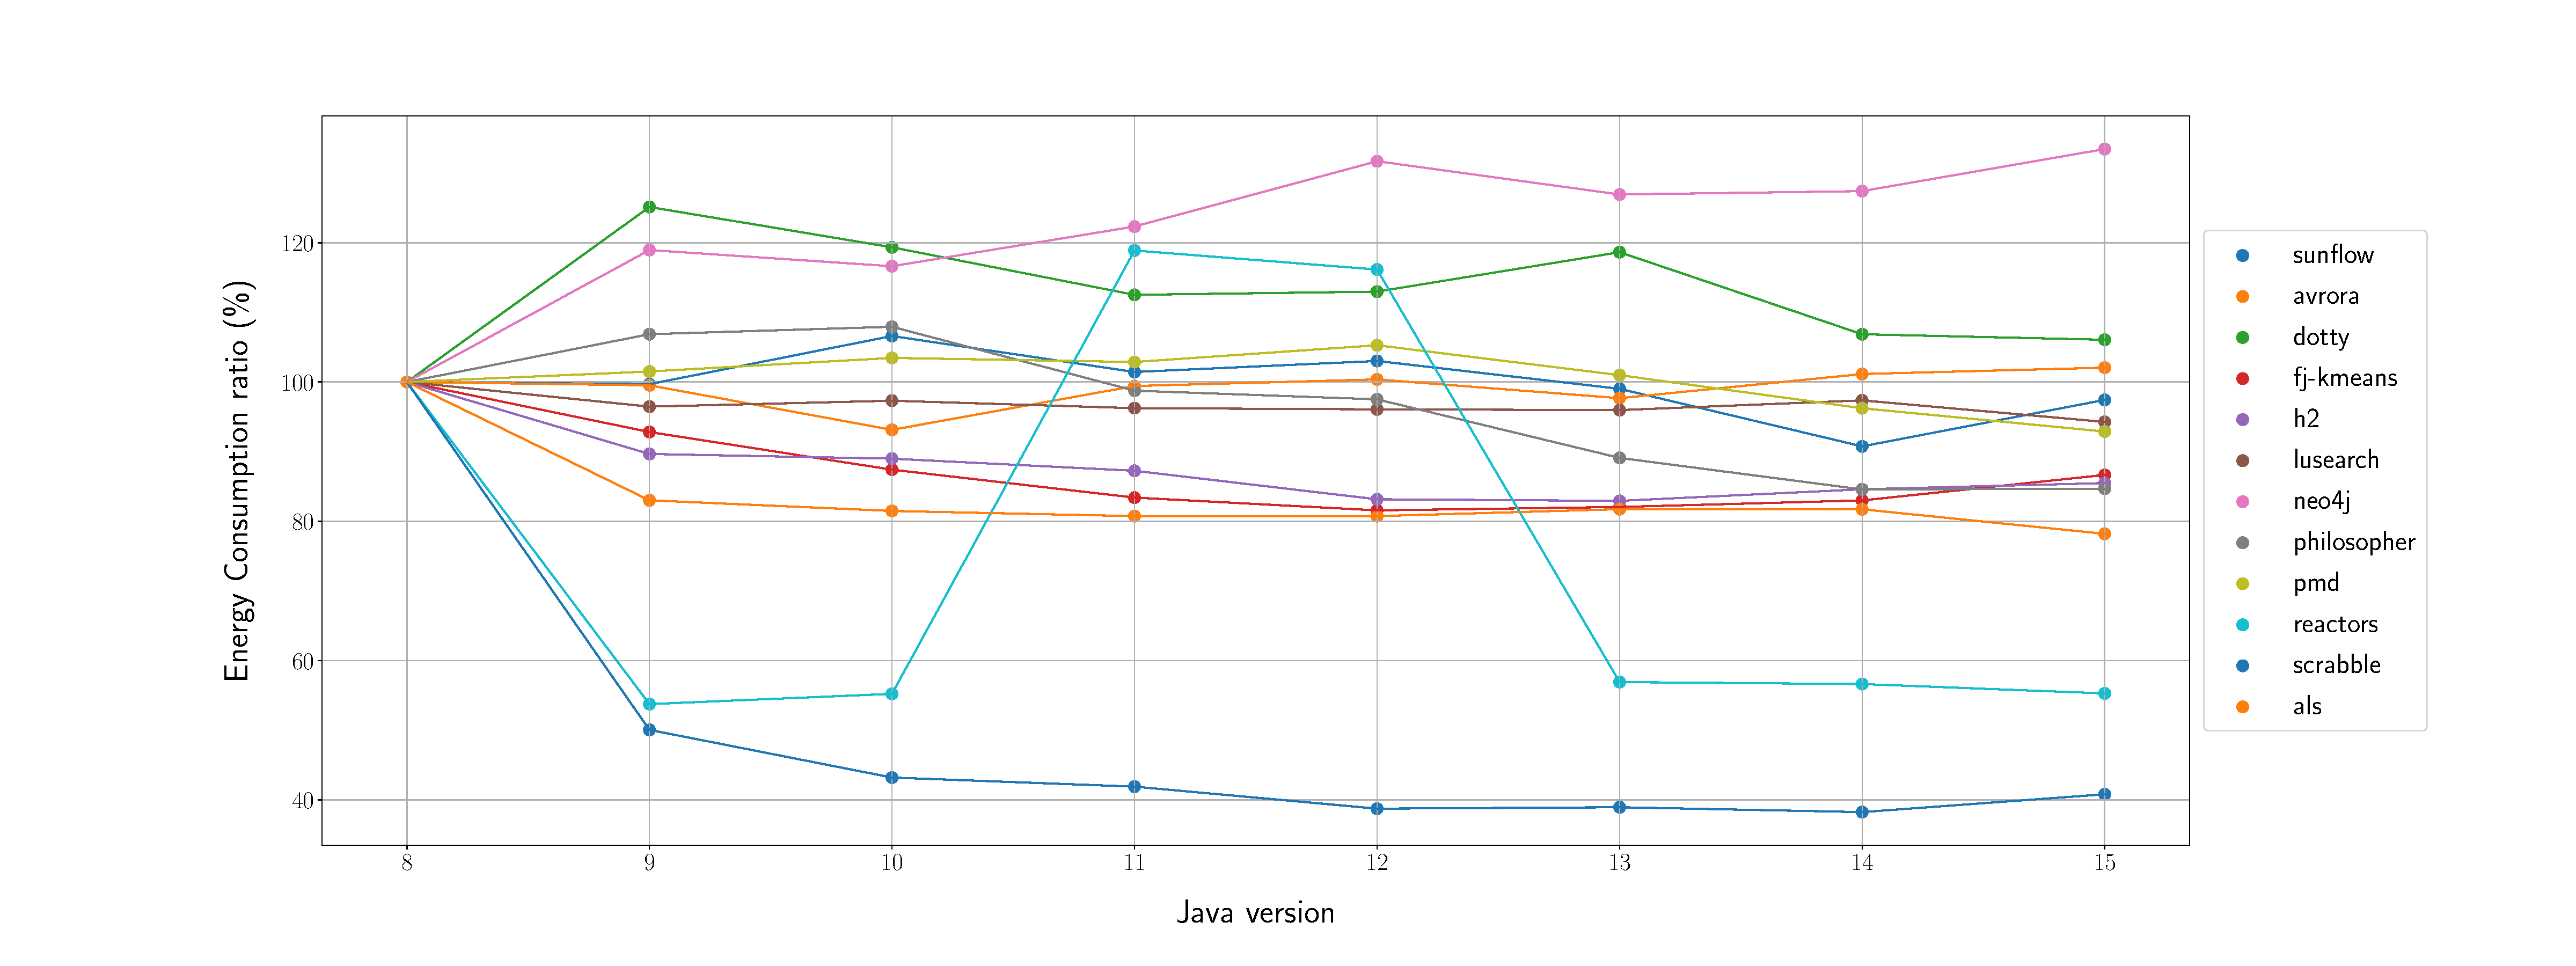
\includegraphics[width=\linewidth]{imgs/lineplothotspot_chetemi8_baseon8}
    \caption{Energy consumption of the HotSpot JVM along versions.}
    \label{fig:hotspot8}
\end{figure*}

% The purpose of this experiment is to check whether the JVM choice can affect the energy consumption of software.
% Yet, the purpose is also to retrieve some mainline information on the JVMs in order to achieve a better energy efficiency.
% Figures \ref{avrora} and \ref{scrabble} depict examples of the energy consumption end execution time of the Avrora and ALS benchmarks respectively.
% We noticed that many of the tested JVMs exhibit similar behaviors and consumption due to the high similarities between these versions.
% In fact, many versions share the same JVM core, and the differences between them are minor (sometimes just packaging changes from a constructor to another) to have any substantial impact in performance or energy consumption.

% \begin{figure*}%[ht]
% 	\begin{subfigure}{\textwidth}
% 		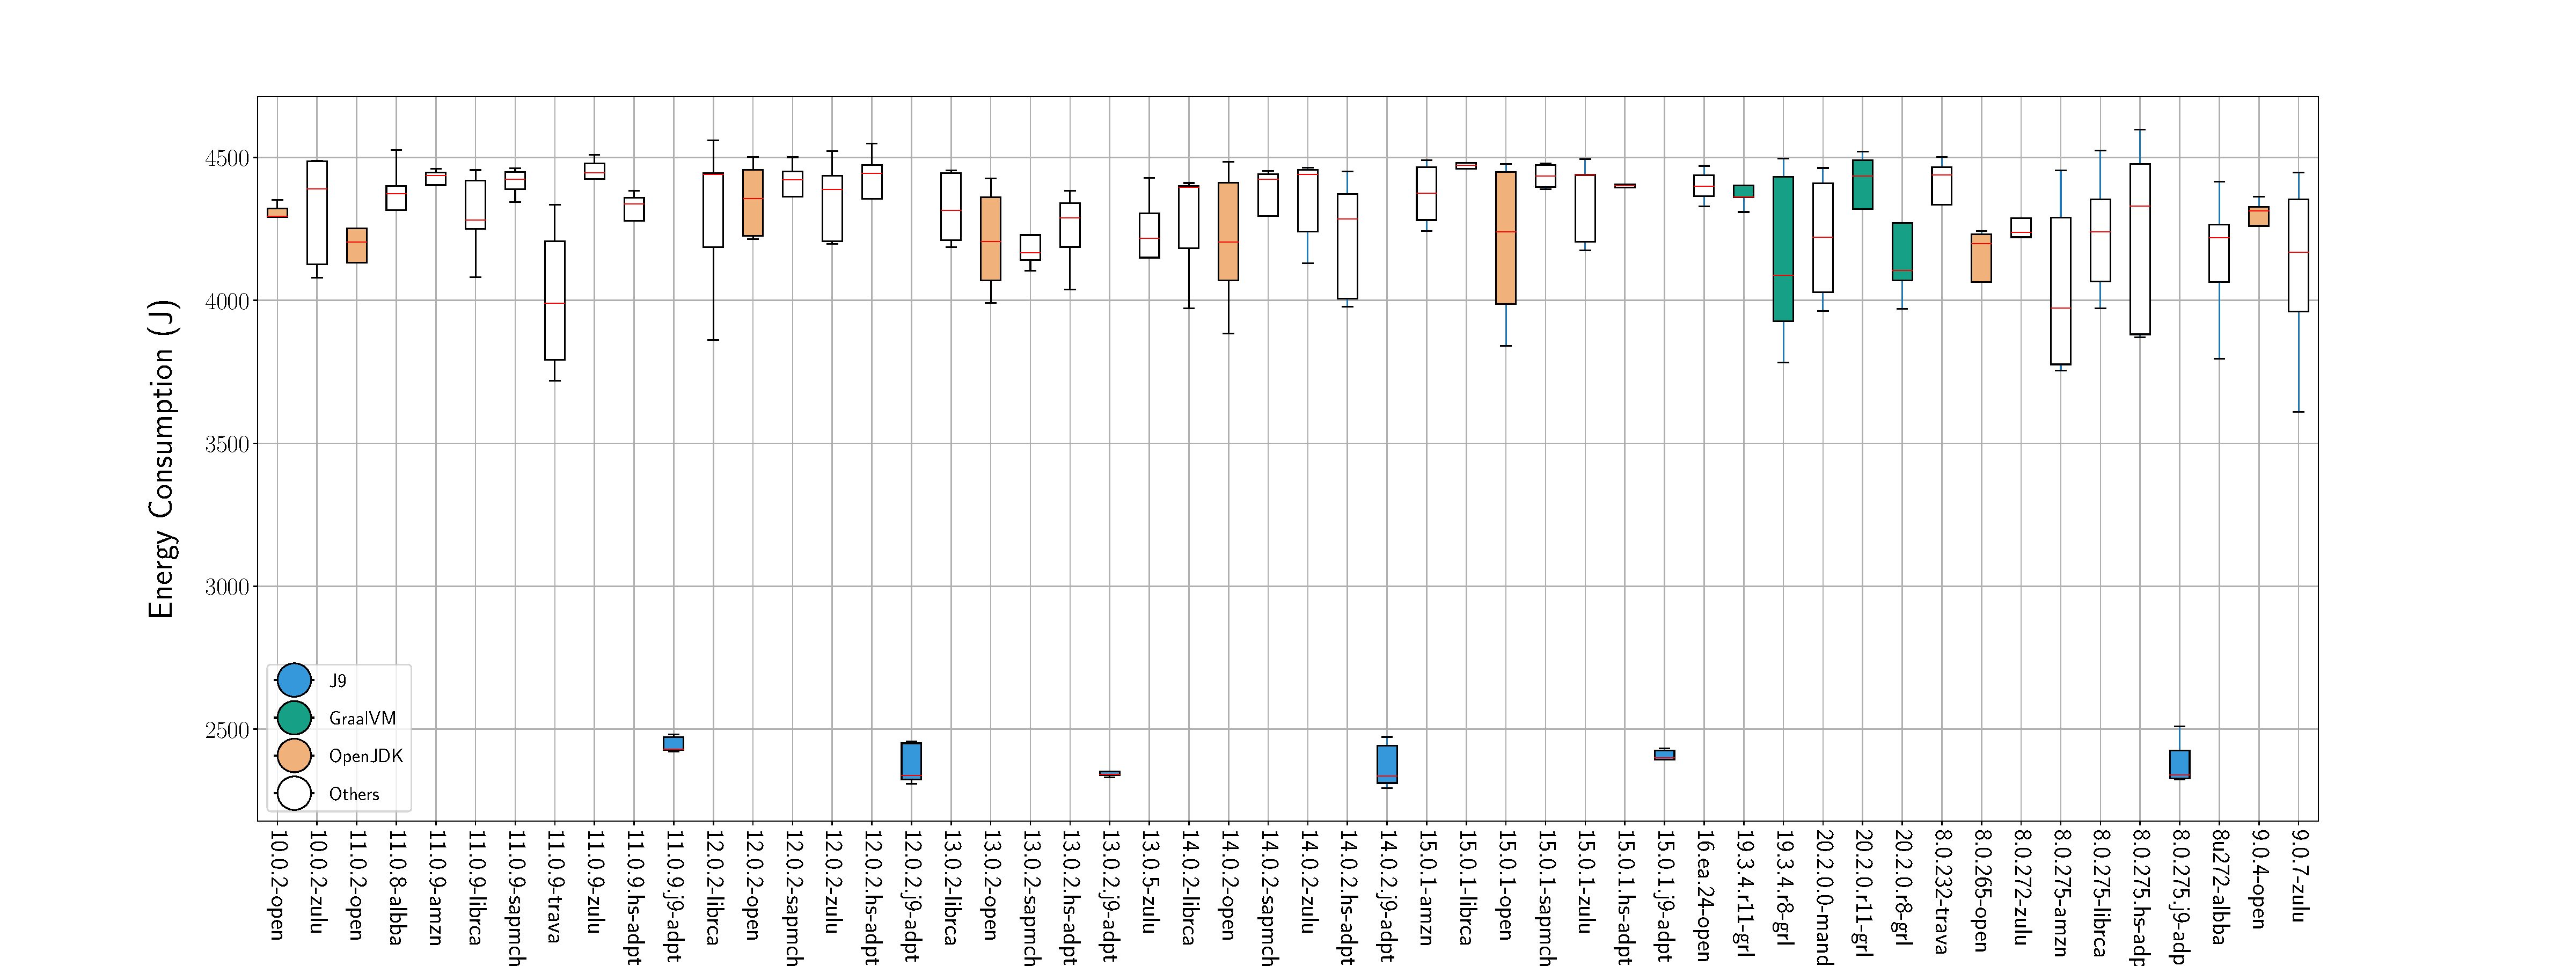
\includegraphics[width=\linewidth]{imgs/energy_pkg_all_avrorachetemi-8.pdf}
% 		\centering
% 		\captionsetup{justification=centering}
% 		\caption{Energy consumption of the Avrora benchmark using the 52 JVMs}\label{fig:avrora_energy}
% 	\end{subfigure}
% 	\begin{subfigure}{\textwidth}
% 		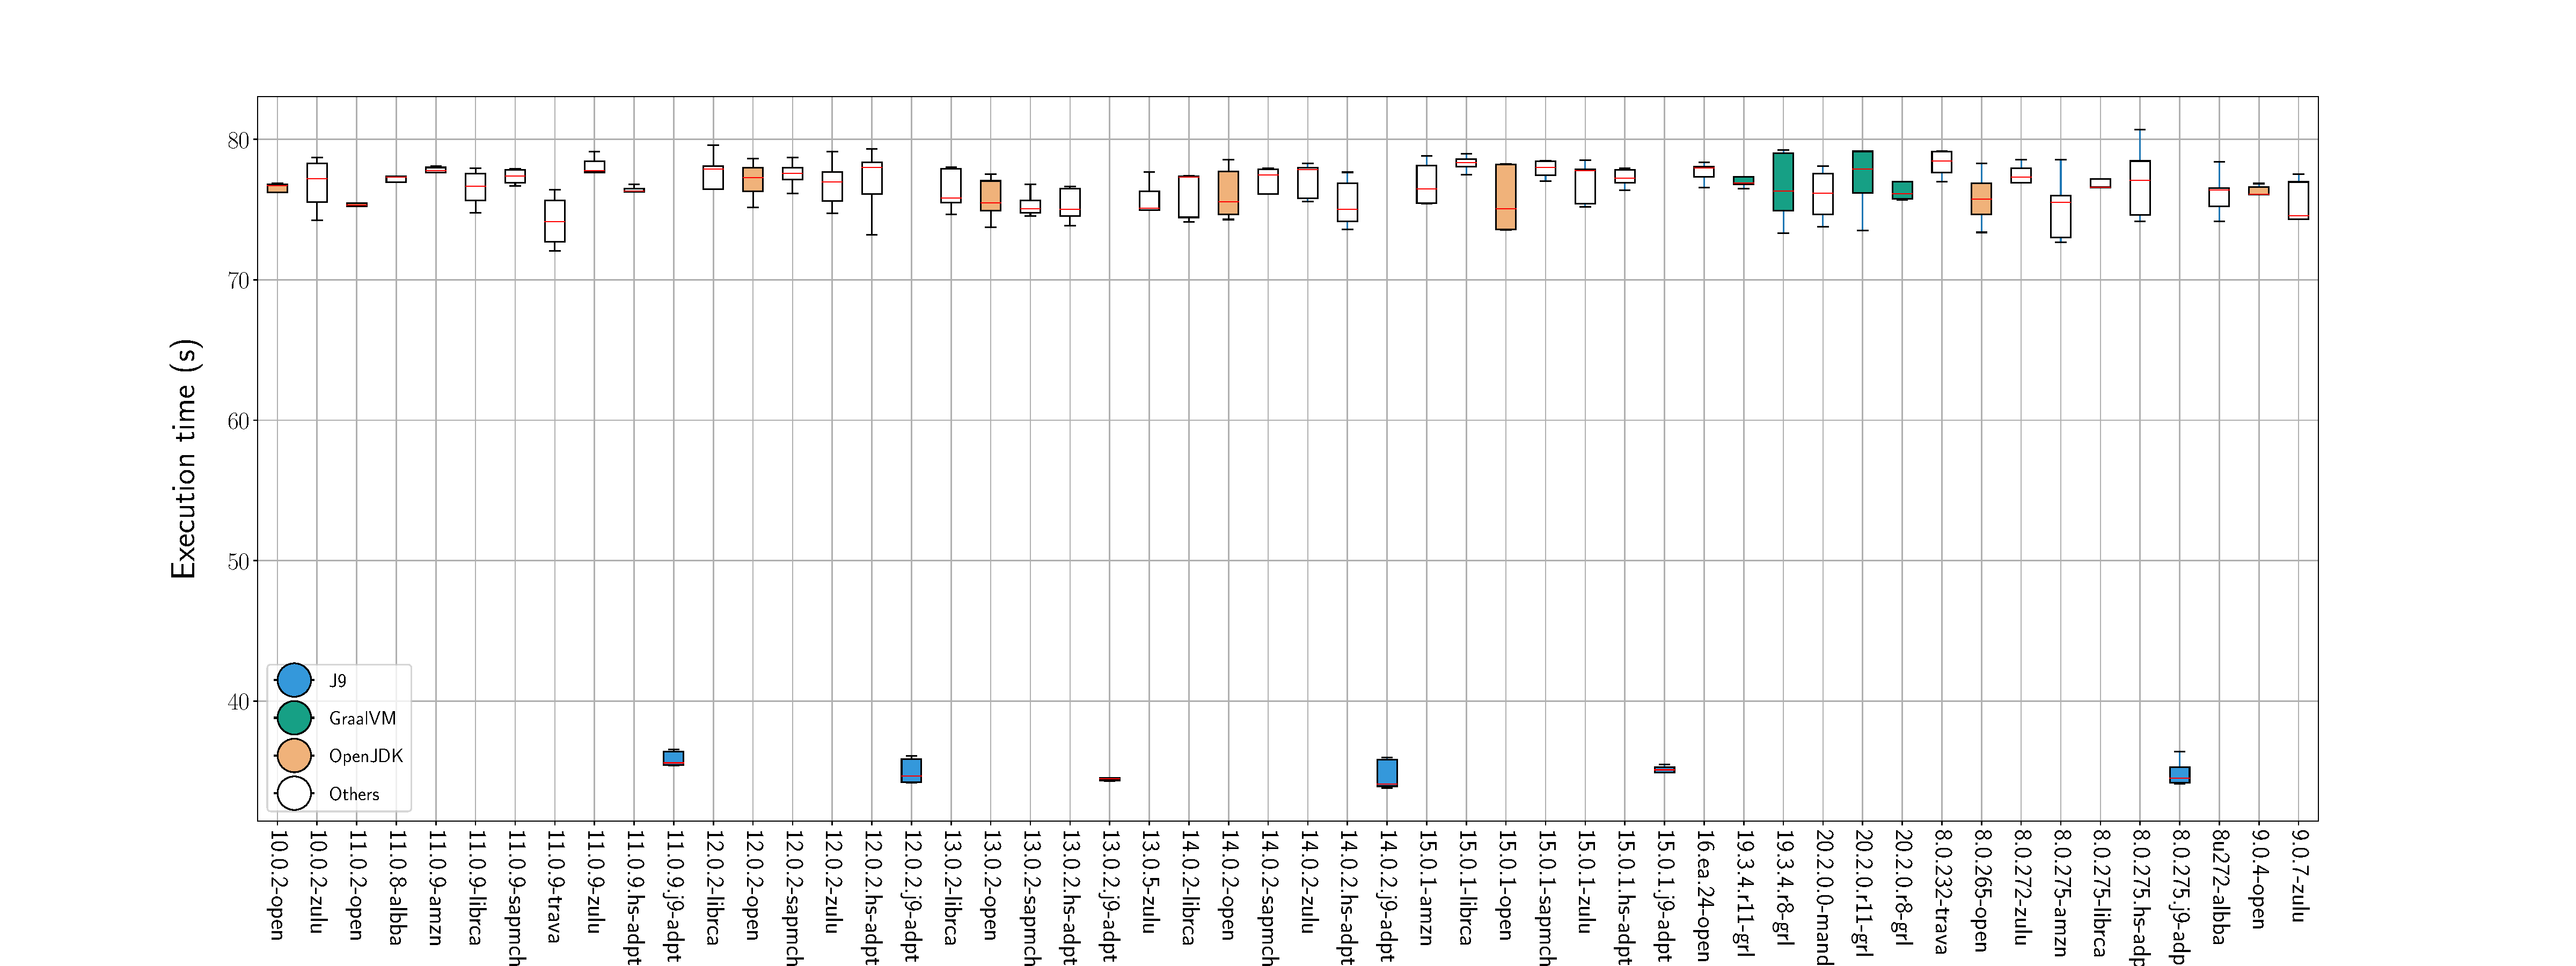
\includegraphics[width=\linewidth]{imgs/execution_time_all_avrorachetemi-8}
% 		\centering
% 		\captionsetup{justification=centering}
% 		\caption{Execution time of the Avrora benchmark using the 52 JVMs}\label{fig:avrora_time}
% 	\end{subfigure}
% 	\caption{Energy consumption and execution time of the Avrora benchmark using the 52 JVMs}
% 	\label{fig:avrora}
% \end{figure*}

% 	\begin{figure*}%[ht]
% 	\begin{subfigure}{\textwidth}
% 		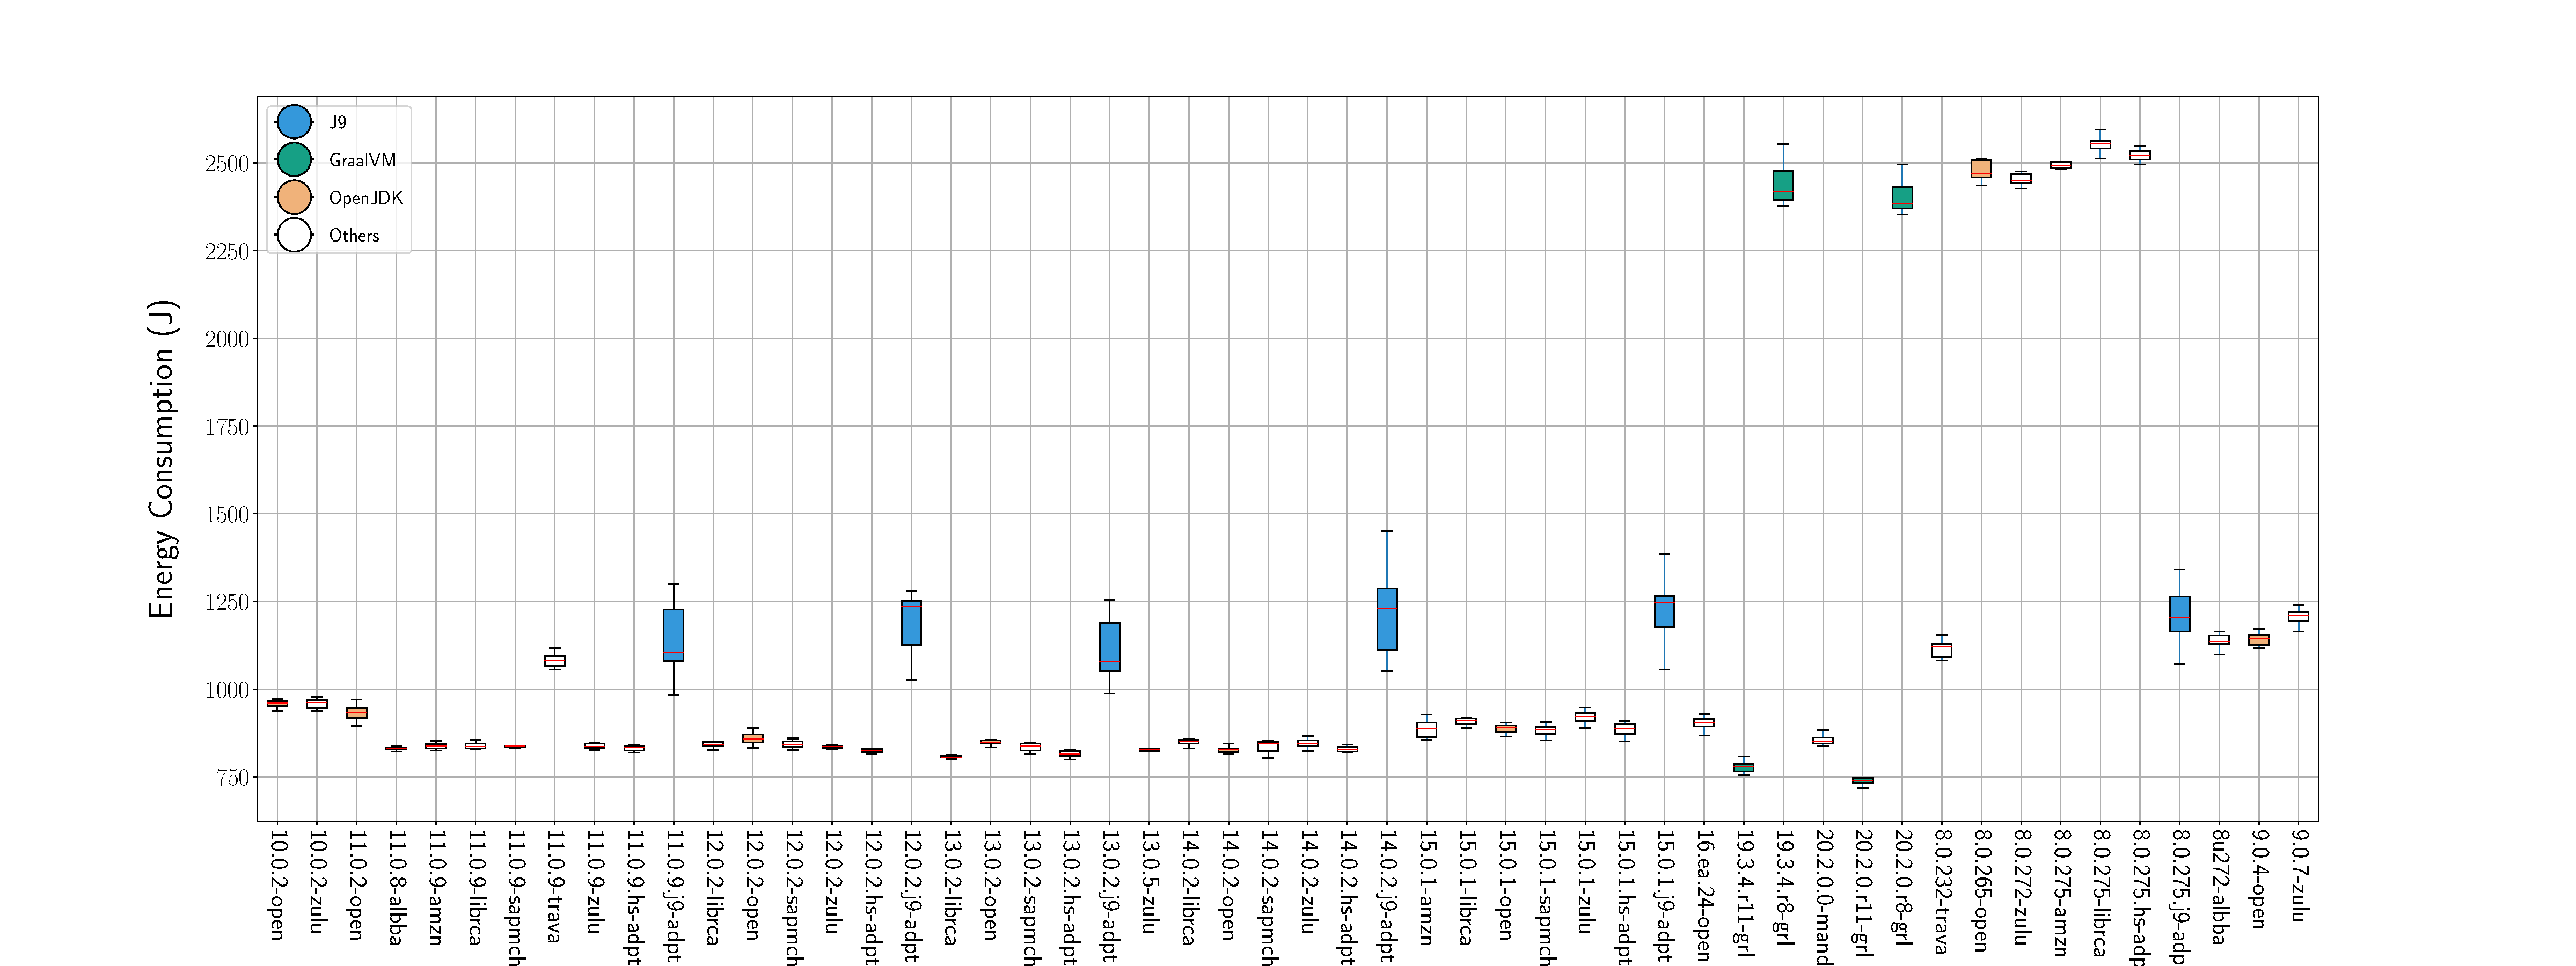
\includegraphics[width=\linewidth]{imgs/energy_pkg_all_scrabblechetemi-8.pdf}
% 		\centering
% 		\captionsetup{justification=centering}
% 		\caption{Energy consumption of the Scrabble benchmark using the 52 JVMs}\label{fig:scrabble_energy}
% 	\end{subfigure}
% 	\begin{subfigure}{\textwidth}
% 		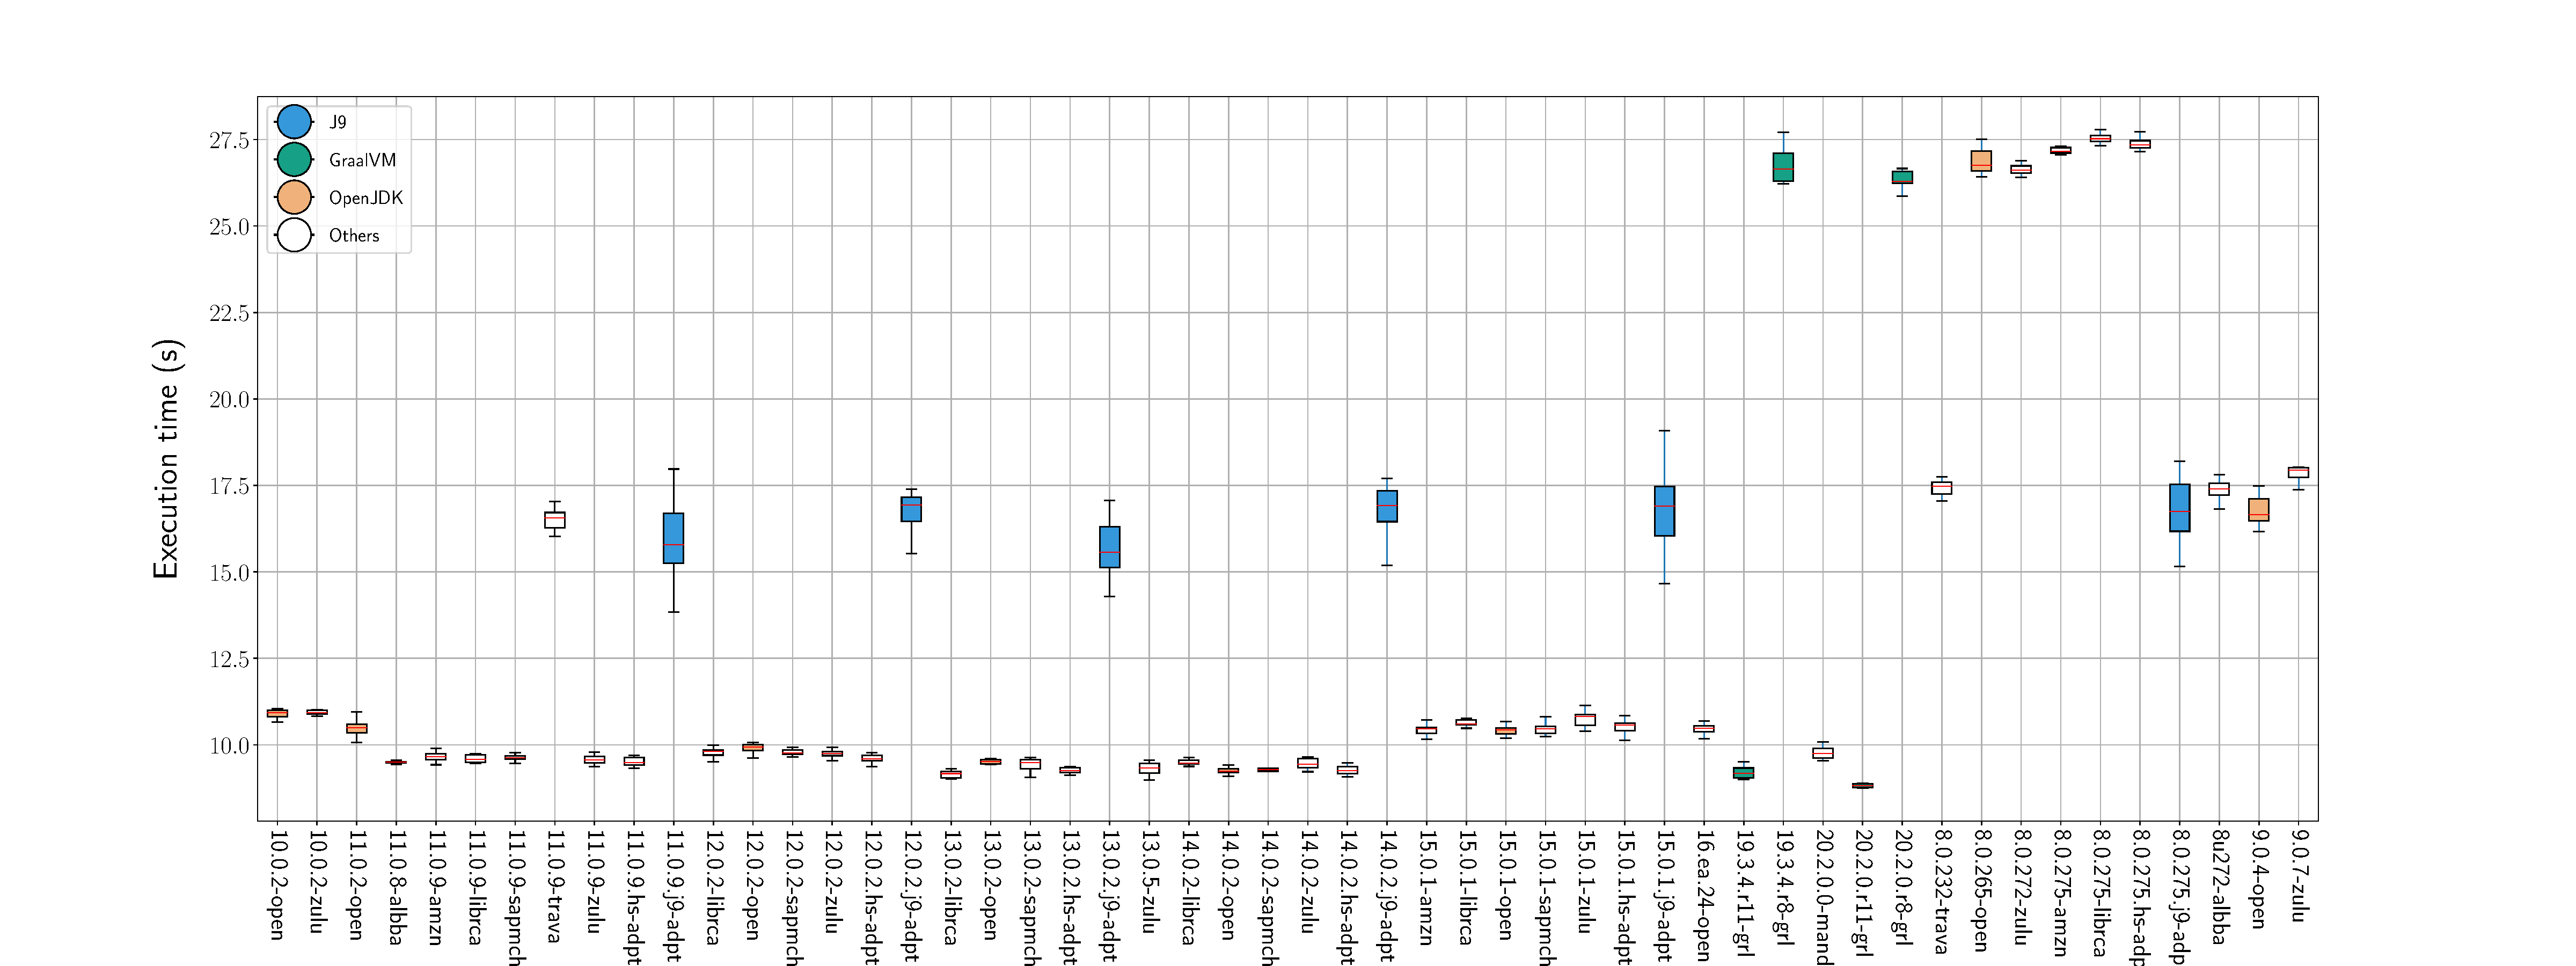
\includegraphics[width=\linewidth]{imgs/execution_time_all_scrabblechetemi-8}
% 		\centering
% 		\captionsetup{justification=centering}
% 		\caption{Execution time of the Scrabble benchmark using the 52 JVMs}\label{fig:scrabble_time}
% 	\end{subfigure}
% 	\caption{Energy consumption and execution time of the Scrabble benchmark using the 52 JVMs}
% 	\label{fig:scrabble}
% \end{figure*}

% We applied those comparison experiments on the whole benchmark set.
% The full results can be found through the anonymous link[footnote].
% Hence, Only 2 JVMs  gave energy consumption results that are different enough to be distinguished from the OpenJDK (GraalVM and J9).

Given that the wide set of distributions and versions seems to highlight 3 classes of energy behaviors, the remainder of this paper considers the following distributions as relevant samples of JVM to be further evaluated: \textsf{20.2.0.r11-grl} (\textsc{GraalVM}), \textsf{15.0.1-open} (\textsc{HotSpot-15}), \textsf{15.0.21.j9} (\textsc{J9}).
We also decided to keep the \textsf{8.0.275-open} (\textsc{HotSpot-8}) as a baseline JVM for some figures to highlight the evolution of energy consumption over time/versions.

\Cref{fig:all_benchs} further explores the comparison of energy efficiency of the JVM distributions per benchmark.
One can observe that, depending on the benchmark's focus, the energy efficiency of JVM distributions may strongly vary.
When considering individual benchmarks, \textsc{J9} performs the worst for at least 6 out of 12 benchmarks---\emph{i.e.}, worst ratio among the 4 tested distributions.
Even though, \textsc{J9} can still exhibit a significant energy saving for some benchmarks, such as \textsf{Avrora}, where it consumes 38\% less energy than \textsc{HotSpot} and others.

\begin{figure*}%[ht]
    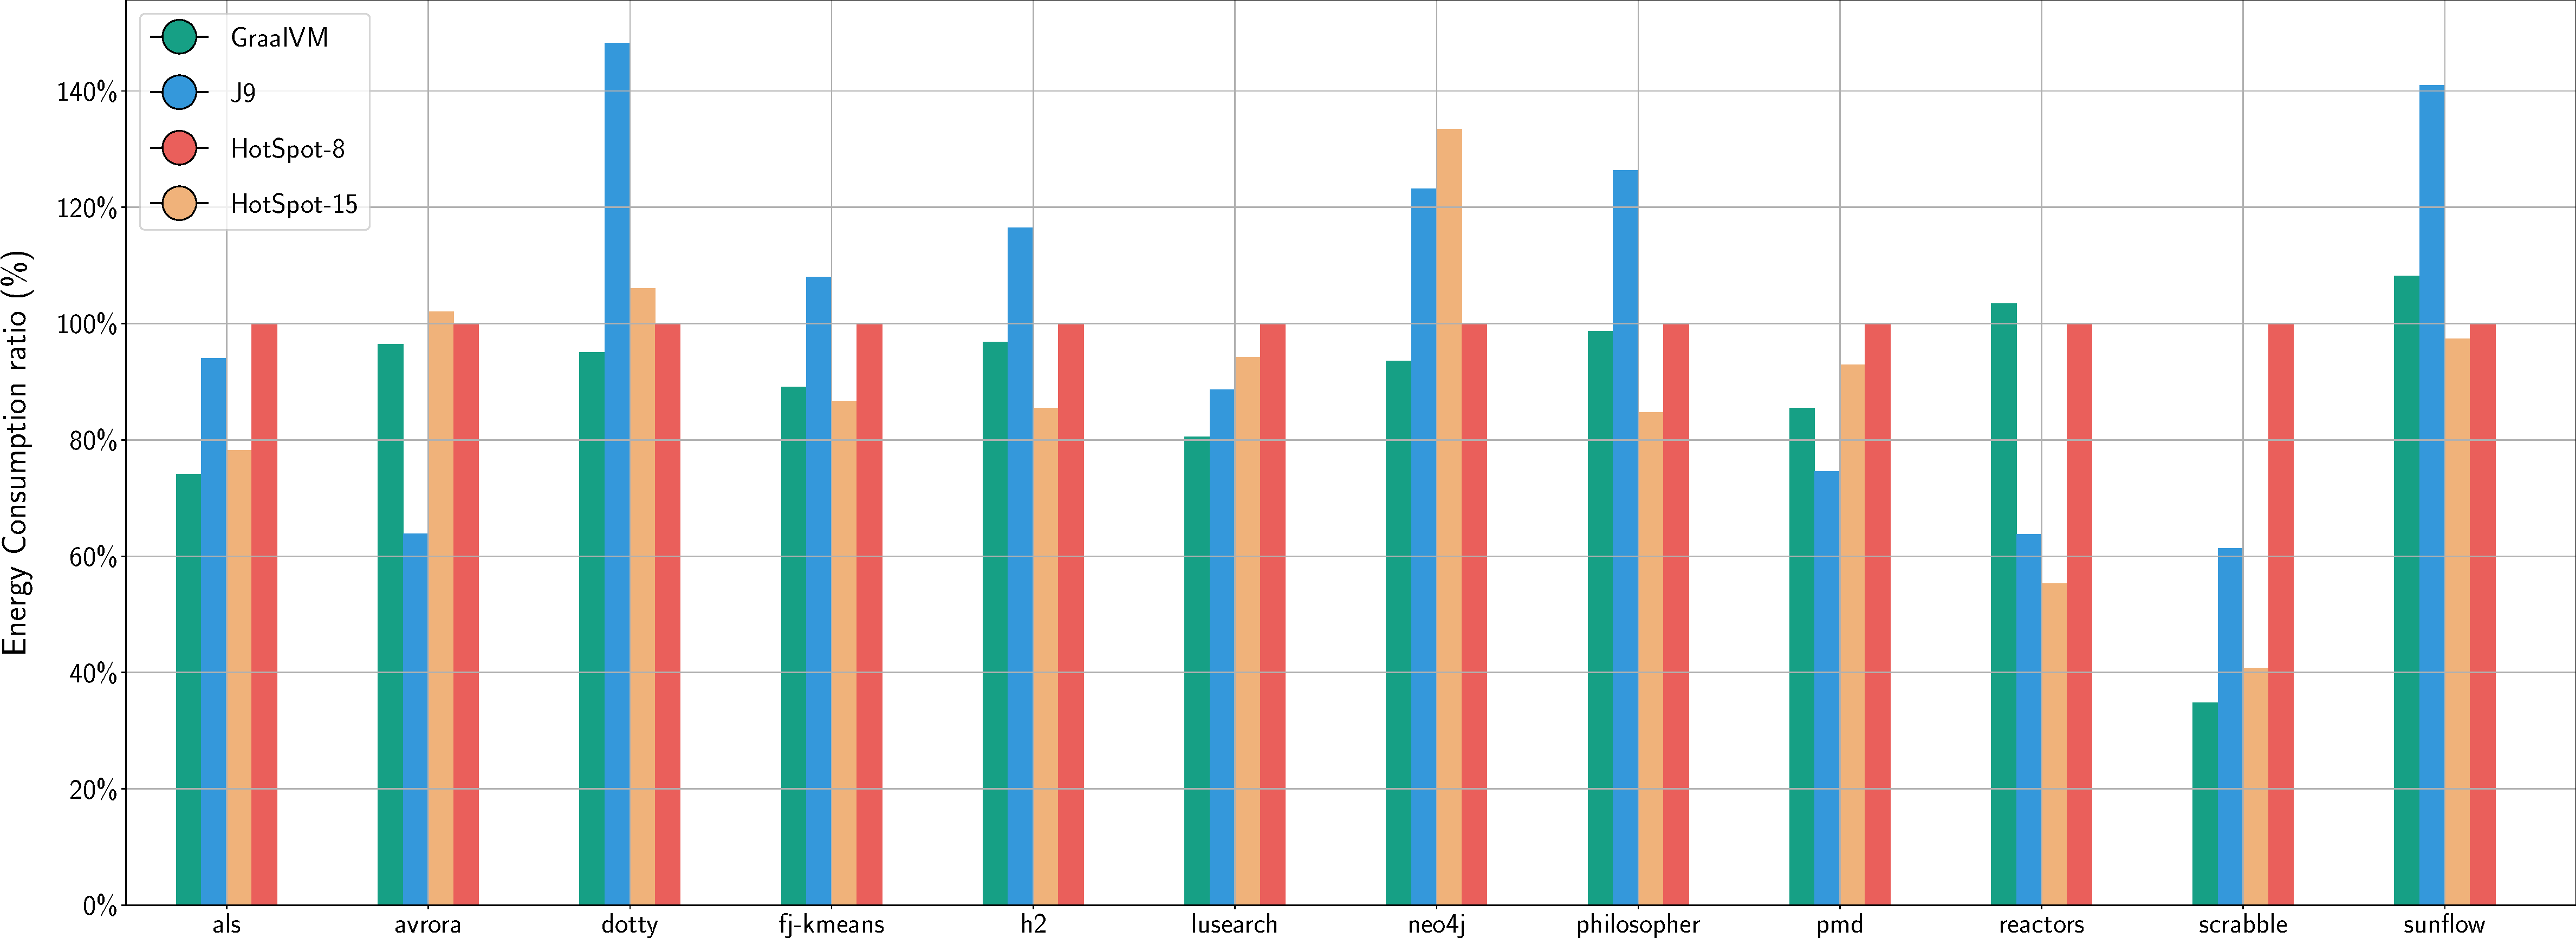
\includegraphics[width=.87\linewidth]{imgs/bar_plot_all_basedon8}
    \centering
    \captionsetup{justification=centering}
    \caption{Energy consumption comparison across Java benchmarks for \textsc{HotSpot}, \textsc{GraalVM} \& \textsc{J9}.}
    \label{fig:all_benchs}
\end{figure*}

Interestingly, \textsc{GraalVM} delivers good results overall, being among the distributions with a low energy consumption for all benchmarks, except for \textsf{Reactors} and \textsf{Avrora}.
Yet, some differences still can be observed with \textsc{HotSpot} depending on applications.
The newer version of \textsc{HotSpot-15} was averagely good and, compared to \textsc{HotSpot-8}, it significantly enhances energy consumption for most scenarios.
Finally, \textsf{Neo4J} is the only selected benchmark where \textsc{HotSpot-8} is more energy efficient than \textsc{HotSpot-15}.


% We can clearly see through the previous figures \ref{avrora} and \ref{scrabble} that choosing OpenJDK, J9 or GraalVM can have a substantial impact the energy consumption and the execution time.
% % also it is still wildy used 
% In figure \ref{avrora}, the consumed energy to run the Avrora benchmark is 44\% less when using the J9 JVM.
% Moreover, we can even see that Avrora executions are running faster on J9 compared to the other platforms .
% In figure\ref{scrabble}, It is noticeable that the GraalVm with version 11 of Java is running 10\% faster and consuming 15\% less energy compared to other JVMs.


% These results can also be confirmed through many of the other benchmarks as each JVM can exhibit a better energy efficiency for some benchmarks and/or experiments.[ref to the footnote again].
% The results showed that we still can distinguish the 3 main platforms (OpenJDK, J9 and Graal) where noticeable energy consumption differences can be detected.
% Figure \ref{all_benchs} illustrates the ratio of consumed energy for the J9 and GraalVM platforms compared to OpenJDK 15.0.1.
% It clearly shows that the three JVM platforms rarely consume the same energy when running the same task,
% A platform can exhibit the best or worst performance/energy consumption depending the benchmark we tested.
% Overall, and among the 12 benchmarks we tested, GraalVM seemed to be the most interesting JVM energy-consumption wise.
% In fact, GraalVm is the most energy efficient in 5 of the 12 benchmarks, by up to 40\% for the Lusearch benchmark compared to OpenJDK.
% J9 on the other hand recorded the worst energy consumption for 7 of the 12 benchmarks. but gave some interesting results with ~45\% and ~25\% improvement for the Avrora and Pmd benchmarks respectively.
% This endorses the further investigation that has to be done in order to determine the different parameters that can contribute to this difference.
% While openJDK~15 and OpenJDK~8 often show close energy consumption (9 of the 12 benchmarks).
% However the oldest version of OpenJDK can consume half the energy consumption for some cases such as Neo4J, and up to ~80\% and ~130\% more for some other cases such as Reactors an Scrabble respectively.
% This proves that the later versions of OpenJDK doesn't essentially outperforms the older ones. 

% \subsubsection{Energy Impact of JVM Distributions on services}
\vspace{6pt}
\noindent\textbf{Service-oriented applications.}
% The previous experiments have been conducted on deterministic jobs where we measured the energy consumption of many runs.
In this section, instead of considering bounded execution of benchmarks, we run the same benchmarks as services for 20 minutes, and we compare the average power and total requests processed by each of the 3 JVM distributions.
Globally, the results showed that the average power when using \textsc{GraalVM}, \textsc{HotSpot}, and \textsc{OpenJ9} is often equivalent and stable over time.
This means that the energy efficiency observed for some JVM distributions with Job-oriented applications is mainly related to shorter execution times, which incidentally results in energy savings.
Nonetheless, we can highlight two interesting observations for two benchmarks whose behaviors differ from others.
First, the analysis of the \textsf{Scrabble} benchmark experiments showed that, in some scenarios, some JVMs can exhibit different power consumptions.
\Cref{fig:servicescrabble} depicts the power consumed by the 3 JVM distributions for the \textsf{Scrabble} benchmark.
One can clearly see that \textsc{GraalVM} requires an average power of 109\,W, which is 9\,W higher than \textsc{HotSpot-15} and 15\,W higher than \textsc{J9}.
% This average power consumption is stable over time.
When it comes to the number of requests processed by \textsf{Scrabbles} during that same amount of time, \textsc{GraalVM} completes $5,336$ requests, against $3,595$ for \textsc{HotSpot} and $2,603$ for \textsc{J9}, as shown in \Cref{table:power/request}.
The higher power usage for \textsc{GraalVM} helped in achieving a high amount of requests, but also the fastest execution of every, request which was 40\% faster on \textsc{GraalVM}.
Thus, \textsc{GraalVM} was more energy efficient, even if it uses more power, which confirms the results observed in \Cref{fig:all_benchs} for this benchmark.

\begin{table}
    \centering
    \caption{Power per request for \textsc{HotSpot}, \textsc{GraalVM} \& \textsc{J9}.}
    \label{table:power/request}
    \small
    \begin{tabular}{|c|c|c|c|c|}
        \hline
        \textbf{Benchmark}            & \textbf{JVM}     & \textbf{Power\,(P)} & \textbf{Requests\,(R)} & $P/R\,\times\,10^{-3}$ \\
        \hline
        \hline
        \multirow{3}{*}{\sf Scrabble} & \textsc{GraalVM} & 109\,W              & \best 5,336\,req       & \best 20\,mW           \\
        \cline{2-5}
                                      & \textsc{HotSpot} & 98\,W               & 3,595\,req             & 27\,mW                 \\
        \cline{2-5}
                                      & \textsc{J9}      & \best 92\,W         & 2,603\,req             & 35\,mW                 \\
        \hline
        \multirow{3}{*}{\sf Dotty}    & \textsc{GraalVM} & \best 45\,W         & 510\,req               & 88\,mW                 \\
        \cline{2-5}
                                      & \textsc{HotSpot} & \best 45\,W         & \best 597\,req         & \best 75\,mW           \\
        \cline{2-5}
                                      & \textsc{J9}      & 46\,W               & 381\,req               & 120\,mW                \\
        \hline
    \end{tabular}
\end{table}

\begin{figure*}%[ht]
    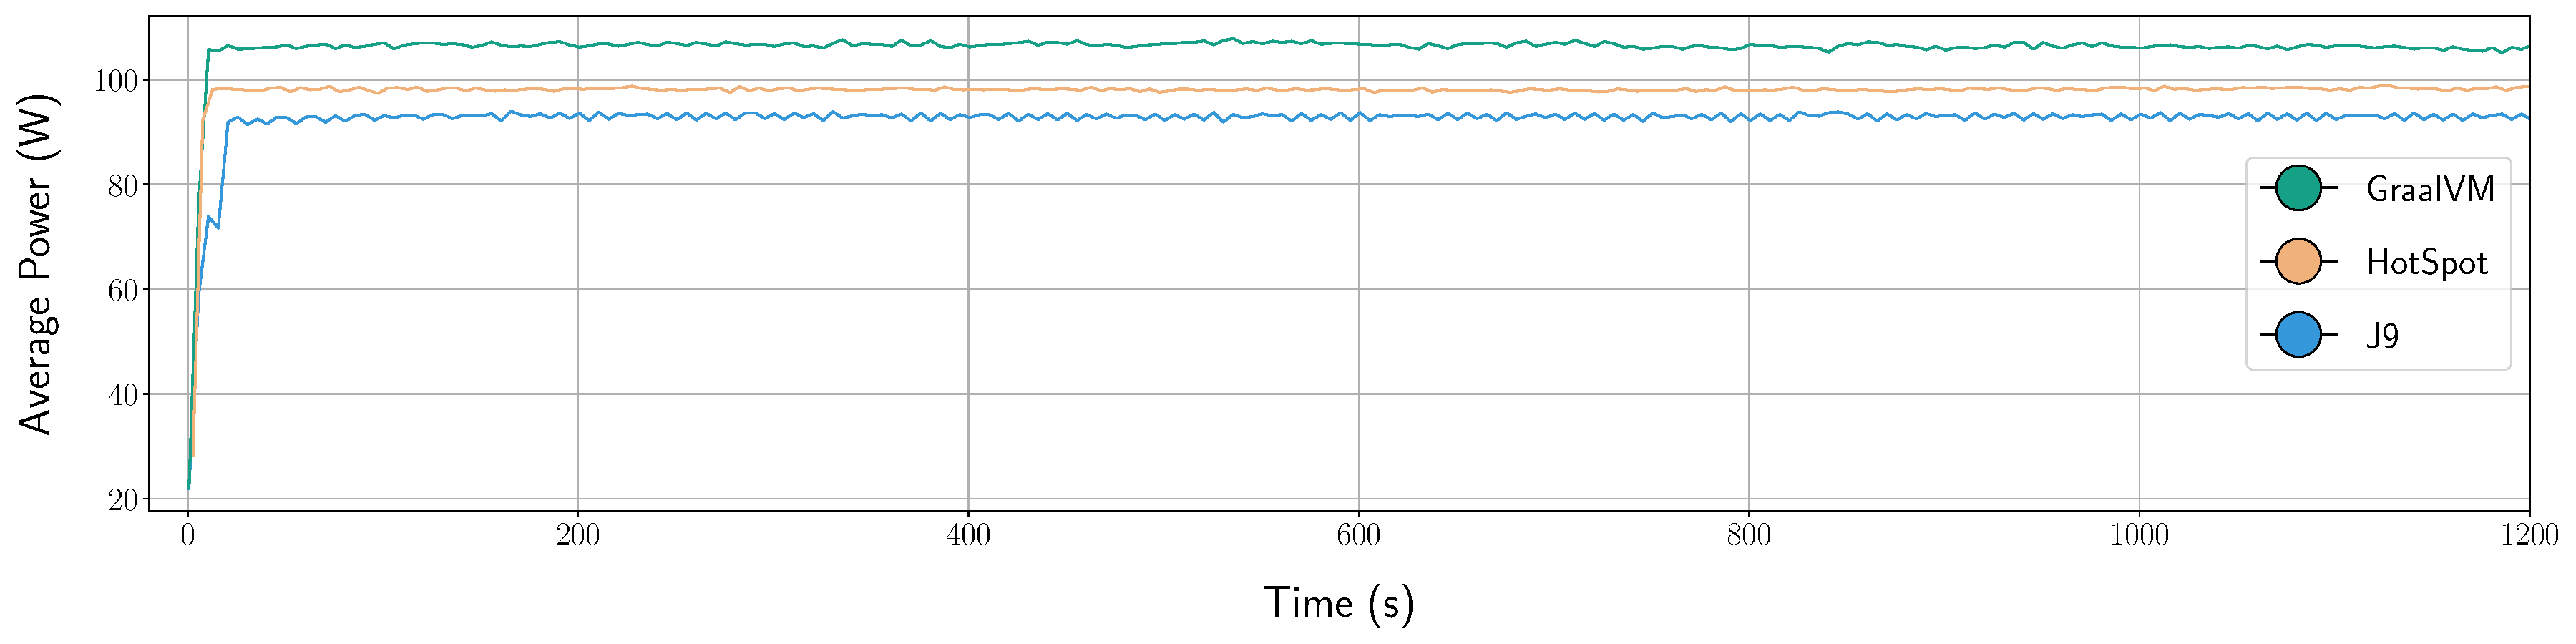
\includegraphics[width=.9\linewidth]{imgs/powers_chetemi-2-scrabble.pdf}
    \centering
    \captionsetup{justification=centering}
    \caption{Power consumption of \textsf{Scrabble} as a service for \textsc{HotSpot}, \textsc{GraalVM} \& \textsc{J9}.}
    \label{fig:servicescrabble}
\end{figure*}

The second interesting situation was observed on the \textsf{Dotty} benchmark.
More specifically, during the first 100 seconds of the execution of the \textsf{Dotty} benchmark on all evaluated JVMs.
At the beginning of the execution, \textsc{GraalVM} has a slightly lower power consumption, is faster, and consumes 10\% less energy.
After about 150 seconds, the power differences between the 3 JVMs is barely noticeable.
One can, however, notice the effect of the JIT, as \textsc{HotSpot} takes the advantage over \textsc{GraalVM} and becomes more energy efficient.
In total, \textsc{HotSpot} completes $597$ requests against $510$ for \textsc{GraalVM} and $381$ for \textsc{J9}, as shown in \Cref{table:power/request}.
\textsc{HotSpot} was thus the best choice on the long term, which explains why it is always necessary to consider a warm-up phase and wait for the JIT to be triggered before evaluating the effect of the JVM or the performance of an application.
This is exactly what we did in our experiments, and why \textsc{HotSpot} was more energy efficient than \textsc{GraalVM} in \Cref{fig:all_benchs}, thus ignoring the warm-up phase would have misleading.

\begin{figure*}%[ht]
    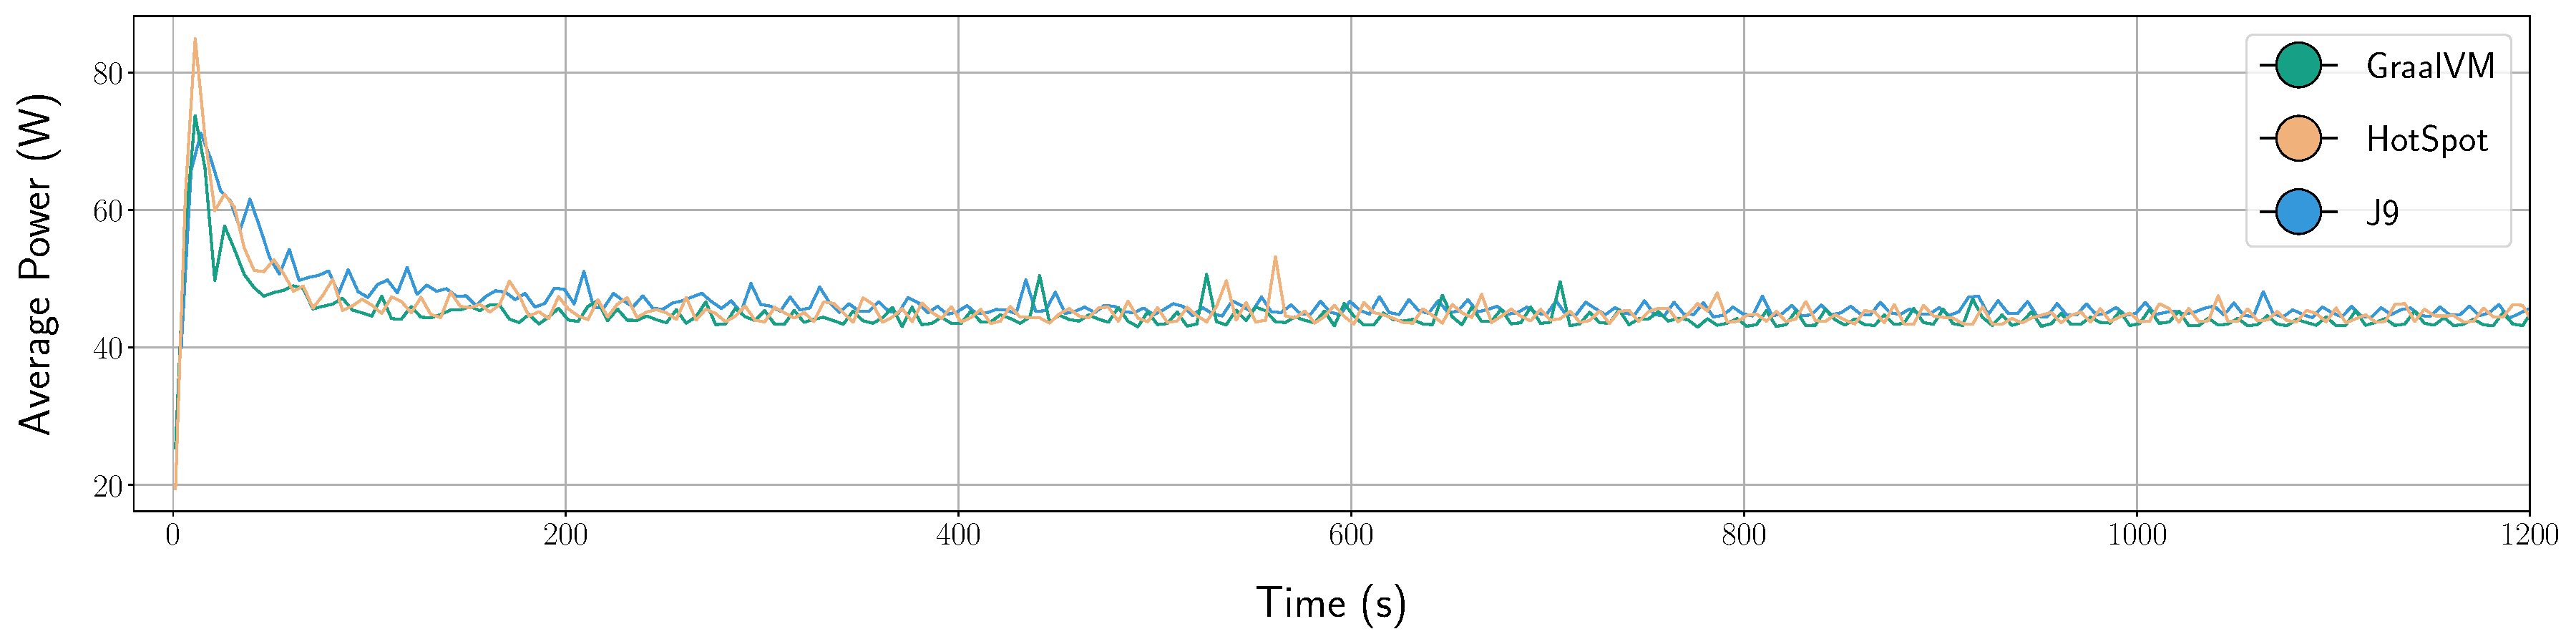
\includegraphics[width=.9\linewidth]{imgs/powers_chetemi-2-dotty.pdf}
    \centering
    \captionsetup{justification=centering}
    \caption{Power consumption of \textsf{Dotty} as a service for \textsc{HotSpot}, \textsc{GraalVM} \& \textsc{J9}.}
    \label{fig:servicedotty}
\end{figure*}
\bigbreak
\begin{mdframed}[]
    To answer \textbf{RQ\,1}, we conclude that---while most of the JVM platforms perform similarly---we can cluster JVMs in 3 classes: \textsc{HotSpot}, \textsc{J9}, and \textsc{GraalVM}.
    The choice of one JVM of these classes can have a major impact on software energy consumption, that strongly depends on the application context.
    When it comes to the JVM version, latest releases tend to offer the lowest power consumption, but experimental features should be carefully configured, thus further questioning the impact of JVM parameters.
\end{mdframed}

\subsection{Energy Impact of JVM Settings}
The purpose of our study is not only to investigate the impact of the JVM platform on the energy consumption, but also the different JVM parameters and configurations that might have a positive or negative effect, with a focus on 3 available settings: multi-threading, JIT, and GC.

\subsubsection{Multithreading}
The purpose behind this phase is to investigate the impact JVM thread management strategies on the energy consumption.
This encompasses exploring if the management strategies of application-level parallelism (so called \emph{threads}) results in different energy efficiencies, depending on JVM distributions.

Investigating such an hypothesis requires a selection of highly parallel and CPU-intensive benchmarks, which is one of the main criteria for our benchmark selection.
As no tool can accurately monitor the energy consumption at a thread level, we monitor the global power consumption and CPU utilization during the execution using RAPL for the energy, and several Linux tools for the CPU-utilization (\texttt{htop}, \texttt{cpufreq}).
%The experiments showed differences in energy consumption between the 3 JVMs and even between 2 version on the HotSpot VM.
Knowing that most of the benchmarks are multi-threaded jobs that use multiple cores, further analysis of thread management is required to understand the results of our previous experiments.
We thus selected the benchmarks that highlighted the highest differences along JVM distributions from \Cref{fig:all_benchs}, namely \textsf{Avrora} and \textsf{Reactors}.
We studied their multi-threaded behavior to optimize their energy efficiency.

\begin{figure*}%[ht]
    \begin{subfigure}{\textwidth}
        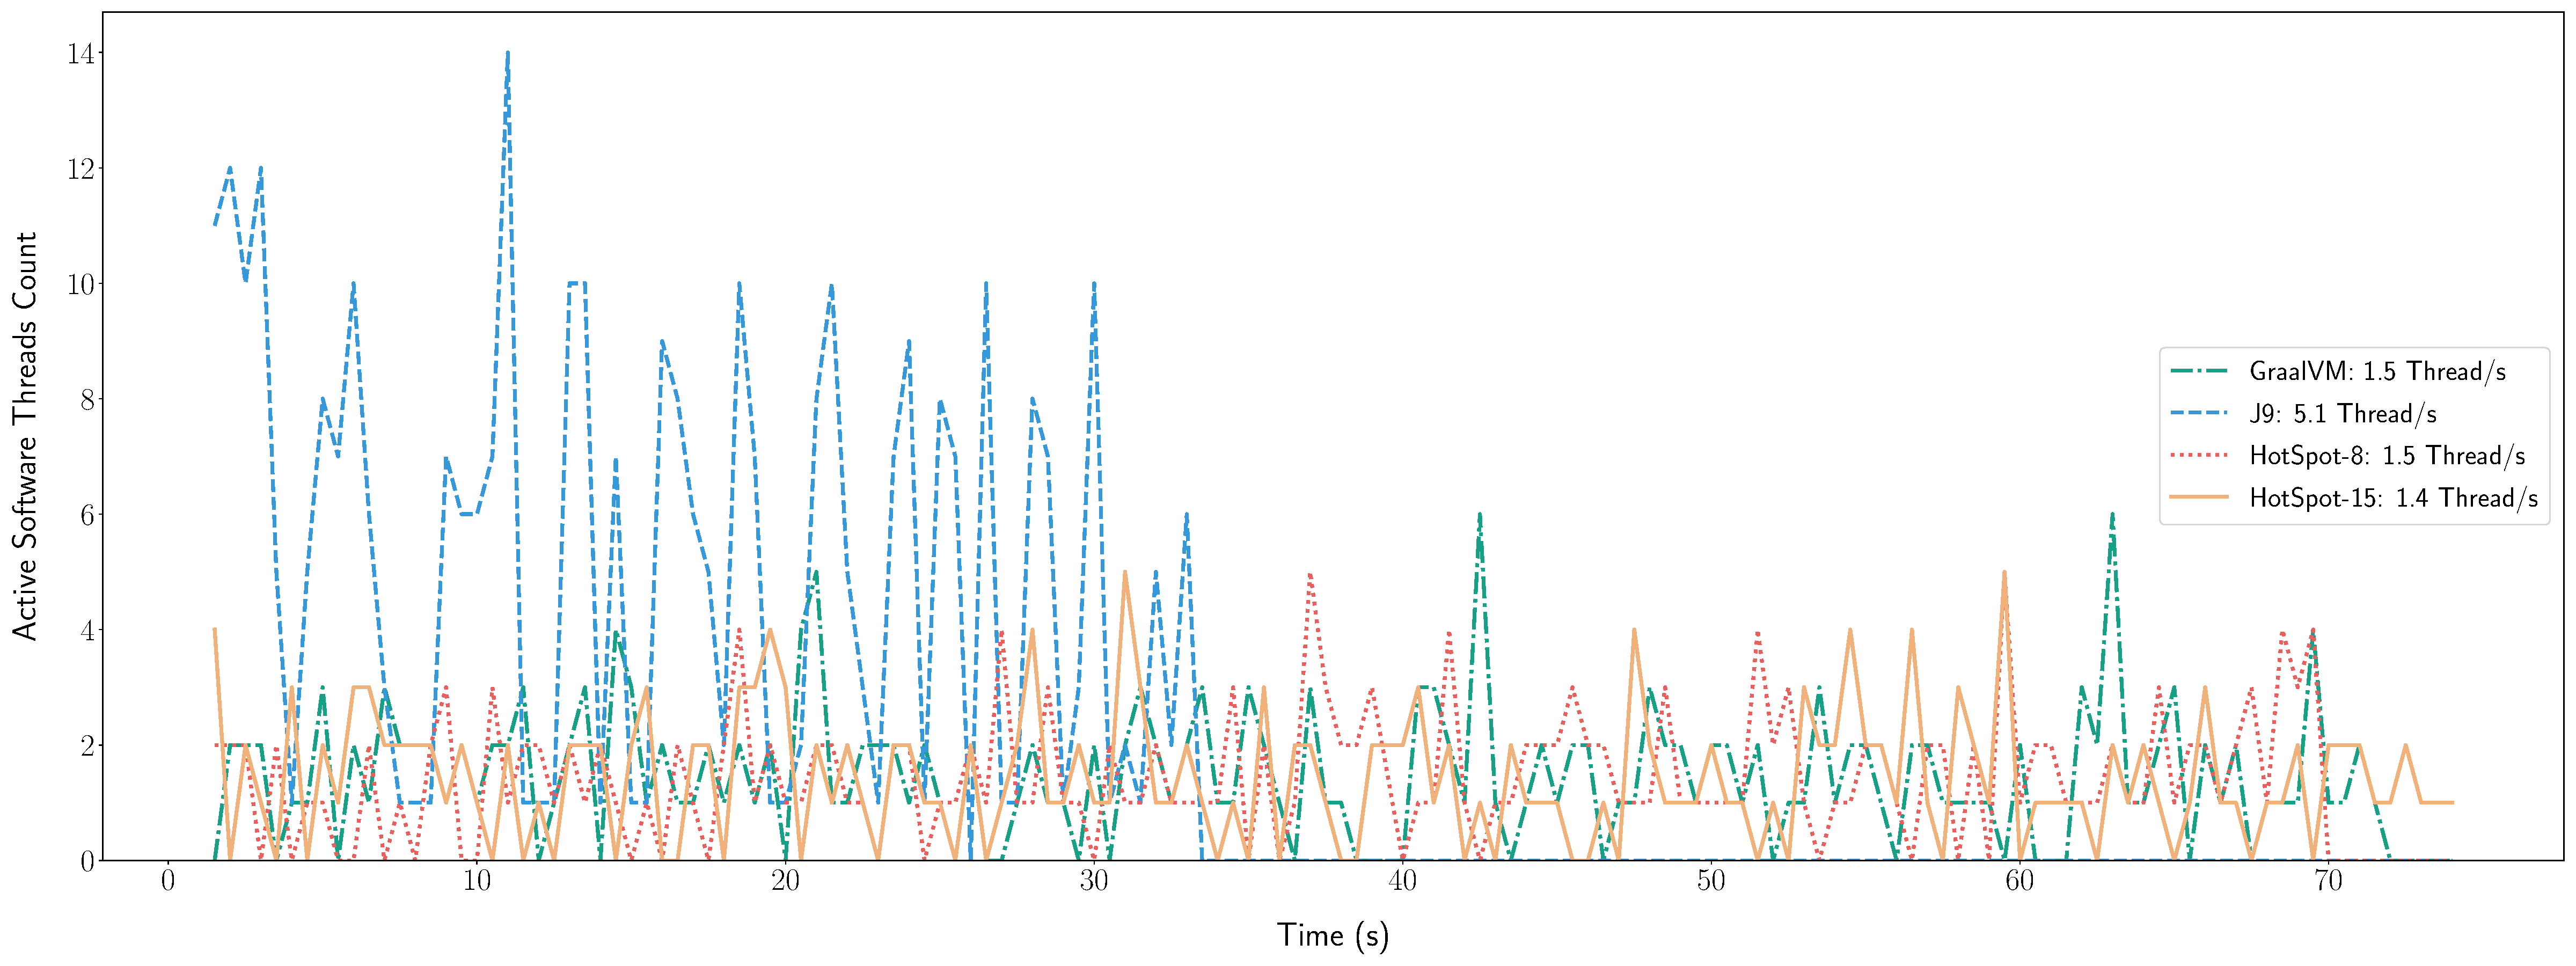
\includegraphics[width=.9\linewidth]{imgs/active_threads_avrora_chetemi_3}
        \centering
        \captionsetup{justification=centering}
        \caption{Active threads of \textsf{Avrora} when using \textsc{HotSpot}, \textsc{GraalVM}, or \textsc{J9}.}
        \label{fig:avrora_threads}
    \end{subfigure}
    \begin{subfigure}{\textwidth}
        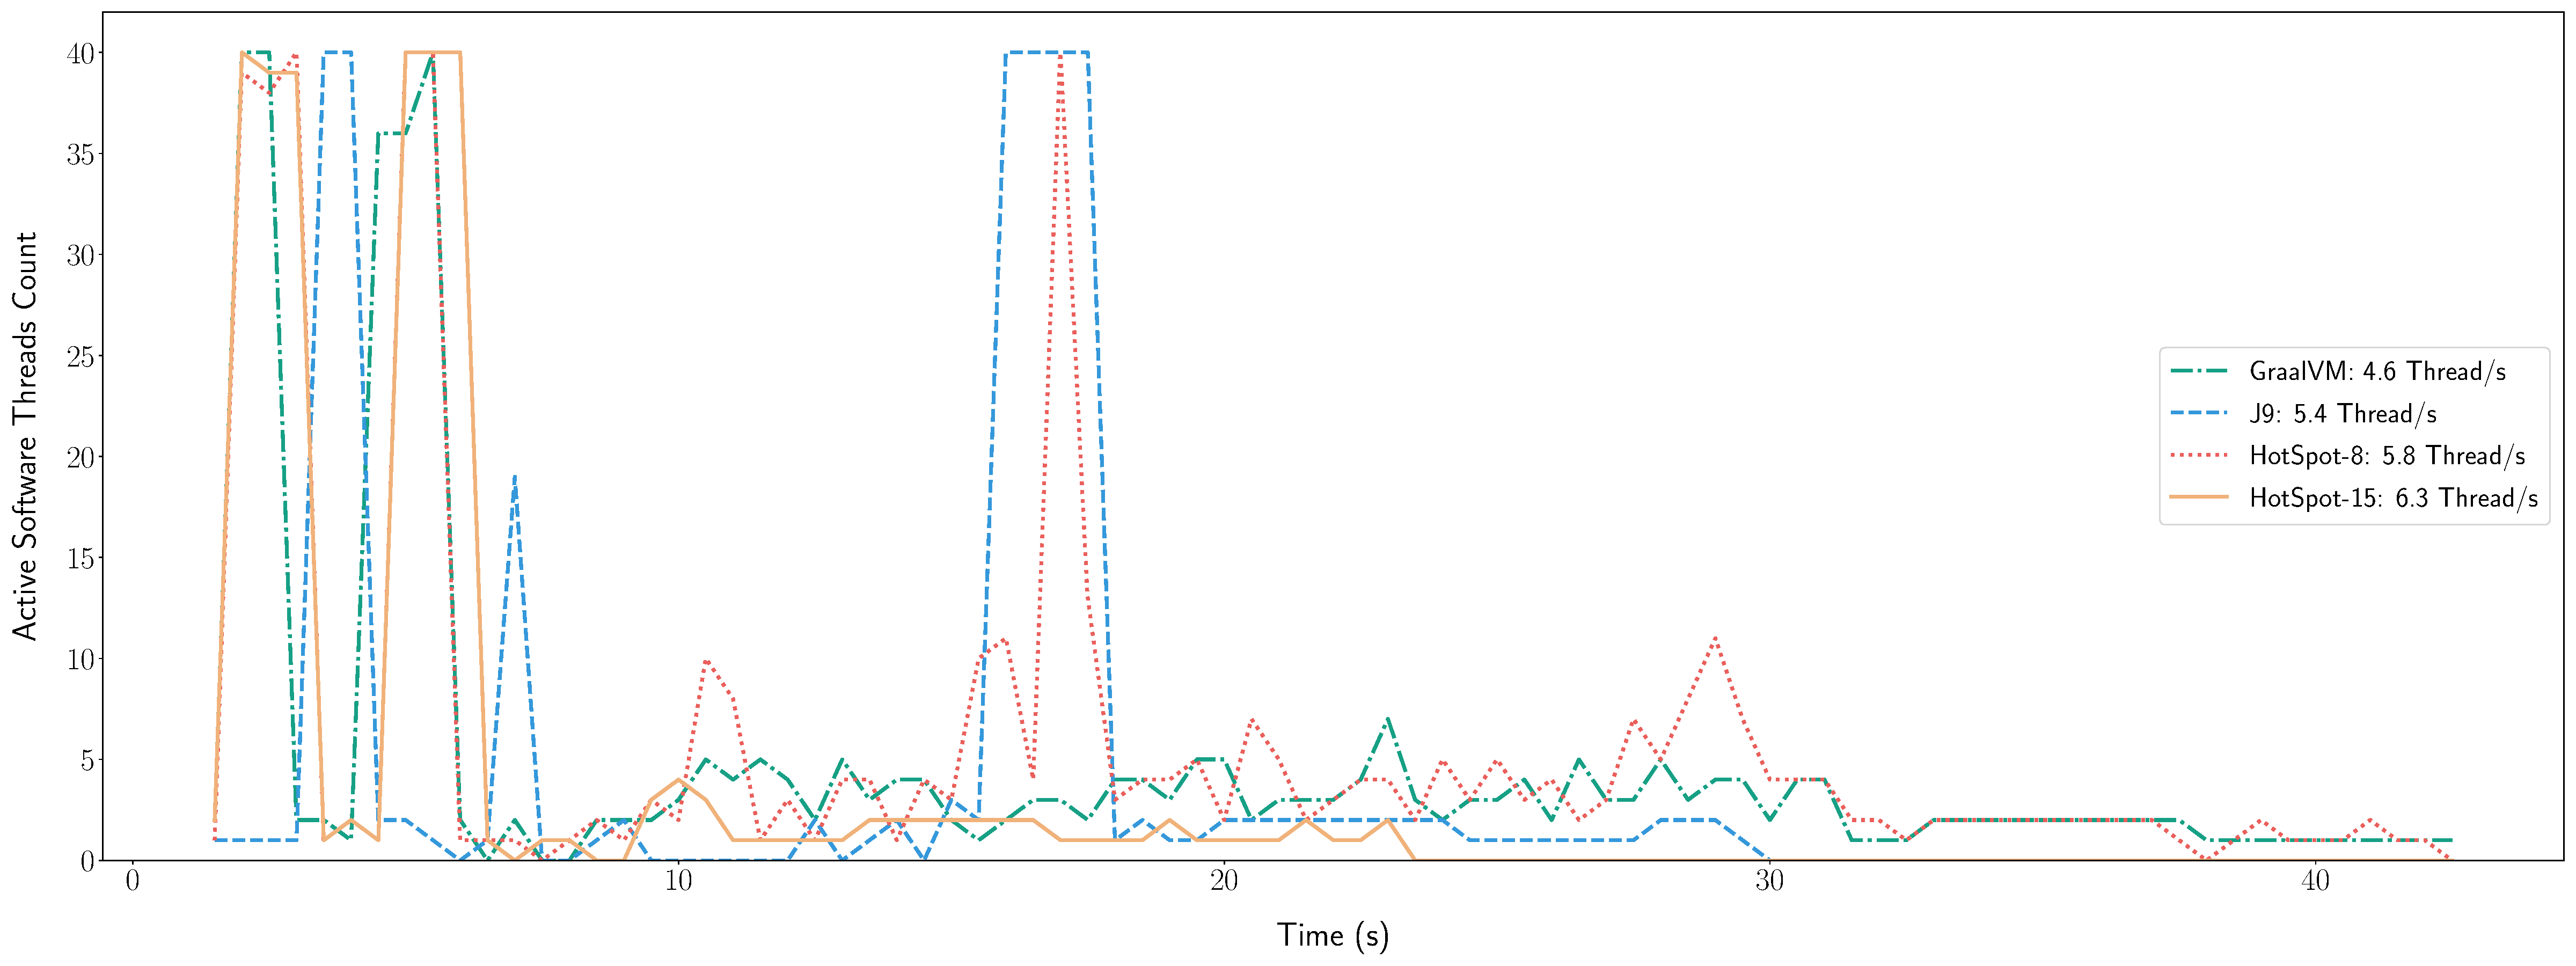
\includegraphics[width=.9\linewidth]{imgs/active_threads_reactors_chetemi_3}
        \centering
        \captionsetup{justification=centering}
        \caption{Active threads of \textsf{Reactors} when using \textsc{HotSpot}, \textsc{GraalVM}, or \textsc{J9}.}
        \label{fig:reactors_threads}
    \end{subfigure}
    %	\begin{subfigure}{\textwidth}
    %		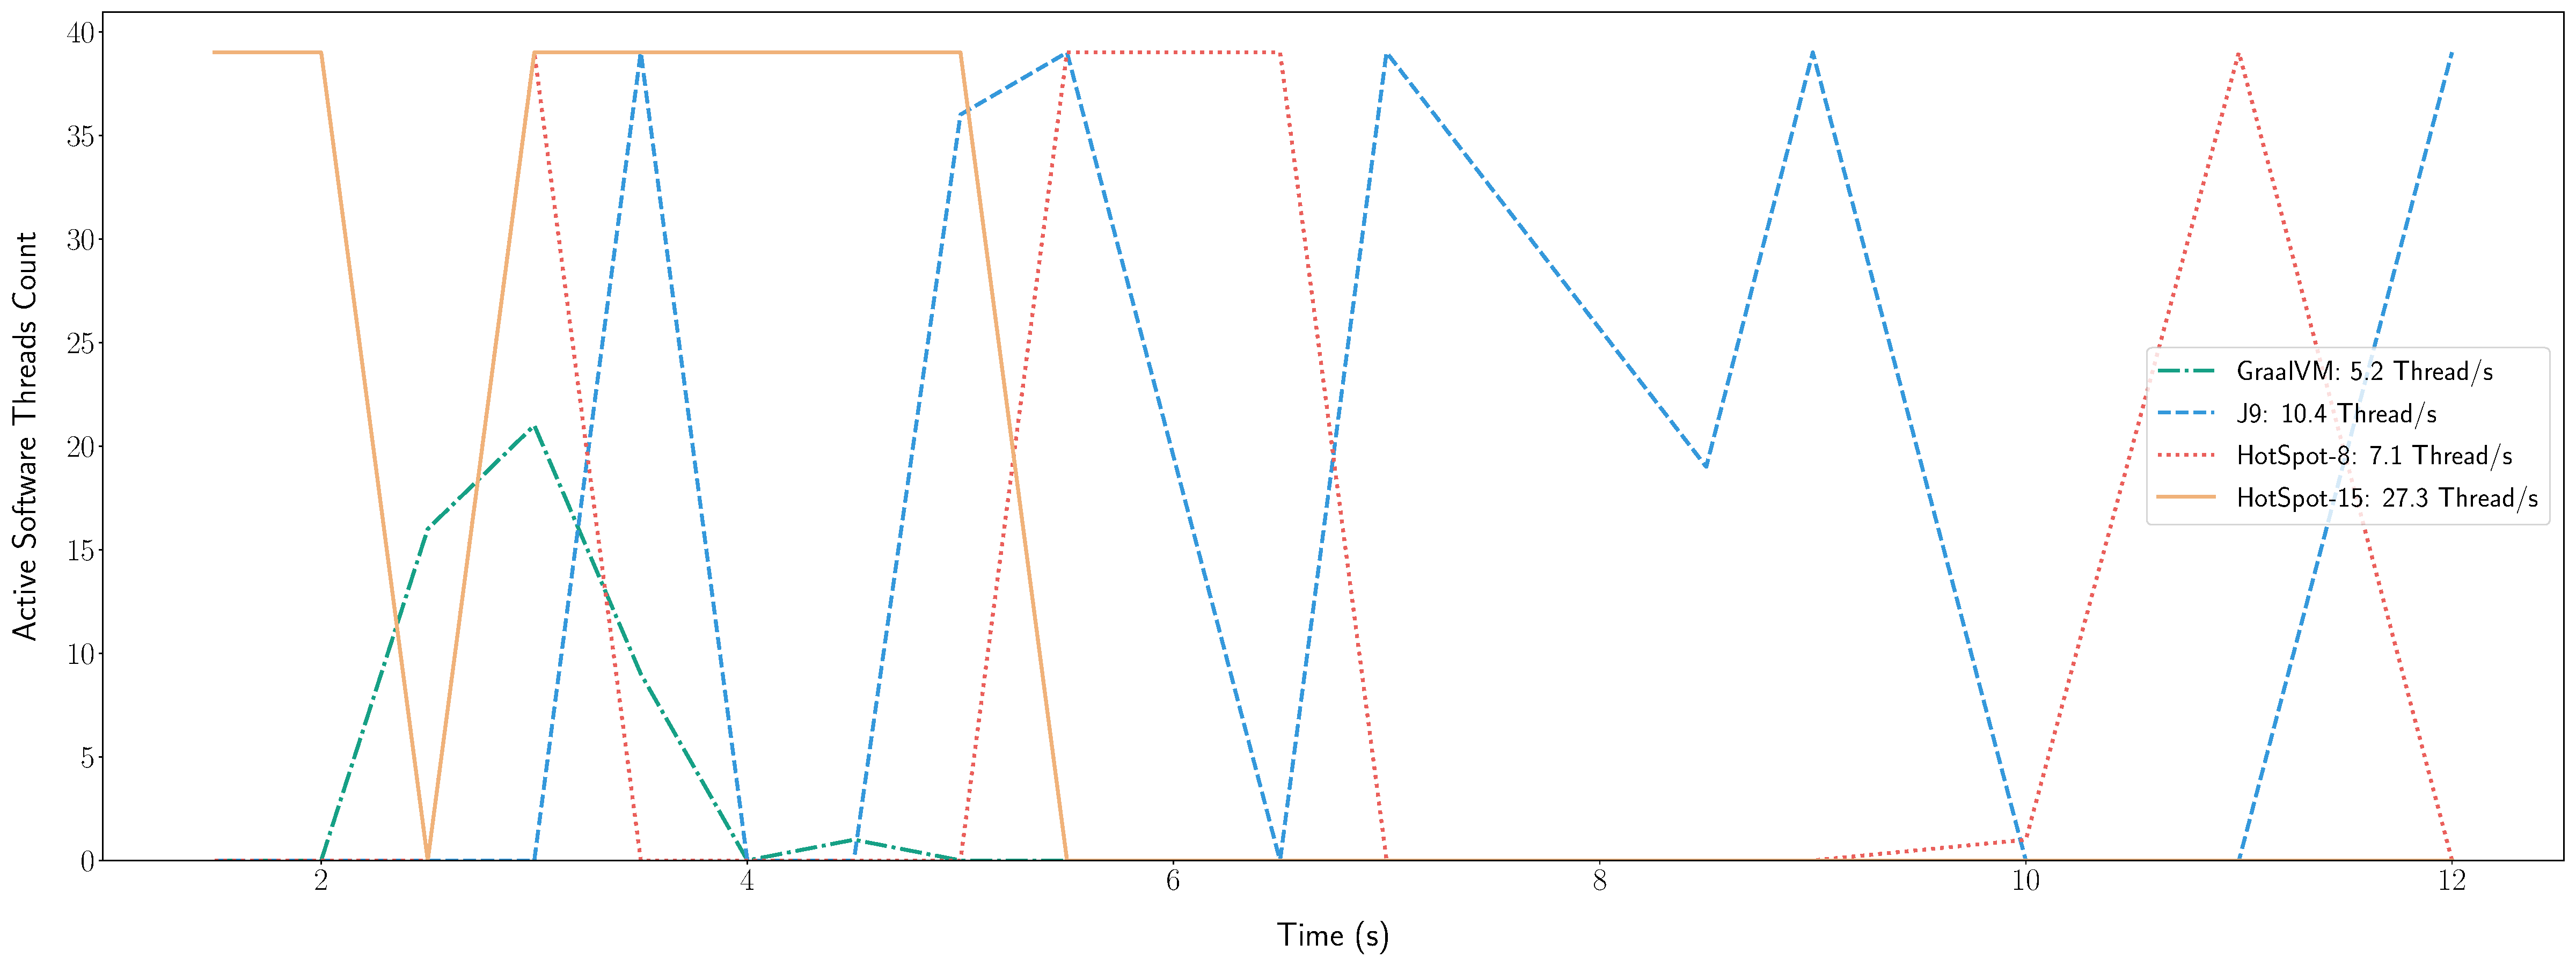
\includegraphics[width=.9\linewidth]{imgs/active_threads_scrabble_chetemi_3.pdf}
    %		\centering
    %		\captionsetup{justification=centering}
    %		\caption{Active threads of \textsf{Scrabble} when using \textsc{HotSpot}, \textsc{GraalVM}, or \textsc{J9}}
    %		\label{fig:scrabble_threads}
    %	\end{subfigure}
    \caption{Active threads evolution when using \textsc{HotSpot}, \textsc{GraalVM}, or \textsc{J9}.}
    \label{fig:threads}
\end{figure*}

\Cref{fig:threads} delivers a closer look to the thread allocation strategies adopted by JVM.
First, \Cref{fig:avrora_threads} illustrates the active threads count evolution over time (excluding the JVM-related threads, usually 1 or 2 extra threads depending on the execution phase) for \textsf{Avrora}.
One can notice through the figure that \textsc{J9} exploits the CPU more intensively by running much more parallel threads compared to other JVMs (an average of 5.1 threads per second for \textsc{J9} while the other JVMs do not exceed 1.5 thread per second).
Furthermore, the number of context switches is twice bigger for \textsc{J9}, while the number of soft page faults is twice smaller.
The efficient \textsc{J9} thread management explains why running the \textsf{Avrora} benchmark took much less time and consumed less energy, given that no other difference for the JIT or GC configuration was spotted between the JVMs.
Another key reasons of the \textsc{J9}'s efficiency for the \textsf{Avrora} benchmark is memory allocation, as \textsf{OpenJ9} adopts a different policy for the heap allocation.
It creates a non-collectable \emph{thread local heap} (TLH) within the main heap for each active thread.
The benefit of cloning a dedicated TLH is the fast memory access for independent threads: each thread has its own heap and no deadlock can occur.

The second example in \Cref{fig:reactors_threads} depicts the active threads evolution over time of the \textsf{Reactors} benchmark.
In this case, all the JVMs have a close average of threads per second.
Nevertheless, one can still observe that \textsc{HotSpot-15} and \textsc{J9} keep running faster, which confirms the results of \Cref{fig:all_benchs}, where both JVMs consume much less energy compared to \textsc{GraalVM} and \textsc{HotSpot-8}.
This difference in energy consumption between benchmarks can be less likely caused by thread management for the \textsf{Reactors} benchmark, as \textsc{HotSpot-8} reports on a higher average of active threads.
However, the TLH mechanism was not as efficient as for the \textsf{Avrora} benchmark, as dedicating a heap for each thread can also cause some extra memory usage for data duplication and synchronization, especially if a lot of data is shared between threads.

%In the case of the \textsf{Scrabble} benchmark illustrated in \Cref{fig:scrabble_threads}, one can see that \textsc{GraalVM} executed the benchmark much faster, and with even less threads.
%With only 5.2 threads/sec, \textsc{GraalVM} was able to be 50\% faster than \textsc{HotSpot-8} and \textsc{J9} and consuming the least energy, while the other JVMs ran more threads per second.
% This advocates that threads management was not the key factor here, thus requiring to further investigate other JVM settings. 
% \textsc{GraalVM} was faster and more energy efficient due to other JVM optimizations.

In conclusion, JVMs thread management can sometimes constitute a key factor that impacts software energy consumption.
However, we suggest to check and compare JVMs before deploying a software, especially if the target application is parallel and multi-threaded.


\subsubsection{Just-in-Time Compilation}
The purpose of experiments on JIT is to highlight the different strategies that can impact software energy consumption within a JVM and between JVMs.
We identified a set of JIT compiler parameters for every JVM platform.

For \textsc{J9}, we considered fixing the intensity of the JIT compiler at multiple levels (\textsf{cold}, \textsf{warm}, \textsf{hot}, \textsf{veryhot}, and \textsf{scorching}).\footnote{\url{[https://www.eclipse.org/openj9/docs/jit/]}}
The hotter the JIT, the more code optimization to be triggered.
We also varied the minimum count method calls before a JIT compilation occurs (\textsf{10}, \textsf{50}, \textsf{100}), and the number of JIT instances threads (from \textsf{1} to \textsf{7}).
For \textsc{Hotspot-15}, we conducted experiments while disabling the tiered complication (that generates compiled versions of methods that collect profiling information about themselves), and we also varied the JIT maximum compilation level from \textsf{0} to \textsf{4}, we also tried out \textsc{HotSpot} with a basic \textsc{GraalVM} JIT.
We note that the level 0 of JIT compilation only uses the interpreter, with no real JIT compilation.
Levels 1, 2, and 3 use the C1 compiler (called client-side) with different amount of extra tuning.
% Furthermore, the level 3 performs a full profiling.
The JIT C2 (also called server-side JIT) compiler only kicks-in at level 4.

For \textsc{GraalVM}, we conducted experiments with and without the JVMCI (a Java-based JVM compiler interface enabling a compiler written in Java to be used by the JVM as a dynamic compiler).
We also considered both the community and economy configurations (no enterprise).
A JIT+AOT (\emph{Ahead Of Time}) disabling experiment has also been considered for all of the 3 JVM platforms.
\Cref{table:JIT} reports on the energy consumption of the experiments we conducted for most of the benchmarks and JIT configurations under study.

\begin{table*}
    \centering
    \caption{Energy consumption when tuning JIT settings on \textsc{HotSpot}, \textsc{GraalVM} \& J9}
    \label{table:JIT}
    \resizebox*{\linewidth}{!}{
        \begin{tabular}{cl|rr|rr|rr|rr|rr|rr|rr|rr|rr|rr}
            \toprule
            JVM & Mode         & \multicolumn{2}{c}{ALS} & \multicolumn{2}{c}{Avrora} & \multicolumn{2}{c}{Dotty} & \multicolumn{2}{c}{Fj-kmeans} & \multicolumn{2}{c}{H2} & \multicolumn{2}{c}{Neo4j} & \multicolumn{2}{c}{Pmd} & \multicolumn{2}{c}{Reactors} & \multicolumn{2}{c}{Scrabble} & \multicolumn{2}{c}{Sunflow}                                                                                                                                      \\
            \midrule
            \multirow{3}{*}{\sc GraalVM}
                & \em Default  & 2848                    & \em p-values               & 3861                      & \em p-values                  & 2271                   & \em p-values              & 948                     & \em p-values                 & 1959                         & \em p-values                & 3313       & \em p-values & 297       & \em p-values & 23452       & \em p-values & 452  & \em p-values & 335       & \em p-values \\
                & DisableJVMCI & 3099                    & \bf 0.001                  & 4012                      & \bf 0.041                     & 2694                   & \bf 0.001                 & \best 934               & \bf  0.011                   & \best 1771                   & \bf 0.005                   & 5086       & \bf  0.001   & 353       & \bf 0.001    & 25007       & \bf 0.007    & 503  & \bf 0.002    & 354       & 0.227        \\
                & Economy      & 4503                    & \bf 0.001                  & 3895                      & 0.793                         & 3466                   & \bf 0.001                 & 1306                    & \bf 0.002                    & 2560                         & \bf 0.001                   & 9525       & \bf  0.001   & \best 270 & \bf 0.001    & 30317       & \bf 0.001    & 649  & \bf 0.002    & 392       & \bf 0.002    \\
            \hline
            \multirow{12}{*}{J9}
                & \em Default  & 3792                    & \em p-values               & 2122                      & \em p-values                  & 3515                   & \em p-values              & 1271                    & \em p-values                 & 2426                         & \em p-values                & 4336       & \em p-values & 277       & \em p-values & 12705       & \em p-values & 734  & \em p-values & 476       & \em p-values \\
                & Thread 1     & 4157                    & \bf 0.001                  & 2121                      & 0.875                         & 4749                   & \bf 0.001                 & 1297                    & 0.097                        & 2597                         & 0.066                       & 4906       & \bf 0.001    & 350       & \bf 0.001    & 12800       & 0.713        & 948  & \bf 0.002    & 626       & \bf 0.005    \\
                & Thread 3     & 3849                    & 0.018                      & 2105                      & 0.713                         & 3574                   & 0.104                     & 1259                    & 0.371                        & 2450                         & 0.637                       & 4477       & \bf 0.005    & 294       & \bf 0.004    & 12647       & 0.875        & 795  & 0.021        & 457       & 0.27         \\
                & Thread 7     & 3843                    & 0.041                      & 2386                      & 0.372                         & 3511                   & 0.875                     & 1259                    & 0.25                         & 2424                         & 0.637                       & 4431       & 0.104        & 273       & 0.372        & 12600       & 0.875        & 808  & 0.055        & 463       & 0.372        \\
                & Count 0      & 8461                    & \bf 0.001                  & 2425                      & \bf 0.001                     & 4877                   & \bf 0.001                 & 2289                    & \bf 0.002                    & 3212                         & \bf 0.001                   & 10565      & \bf 0.001    & 744       & \bf 0.001    & 18084       & \bf 0.001    & 1476 & \bf 0.002    & 922       & \bf 0.001    \\
                & Count 1      & 4281                    & \bf 0.001                  & 2150                      & 0.431                         & 3164                   & \bf 0.001                 & 1841                    & \bf 0.002                    & 2546                         & 0.431                       & 7166       & \bf 0.001    & 272       & 0.128        & 14715       & \bf 0.001    & 1005 & \bf 0.002    & 514       & 0.052        \\
                & Count 10     & 3980                    & \bf 0.001                  & 2431                      & 0.713                         & 3771                   & \bf 0.001                 & 1312                    & \bf 0.011                    & 2779                         & \bf  0.003                  & 4979       & \bf 0.001    & 299       & \bf 0.001    & 12000       & 0.104        & 860  & \bf 0.005    & 1182      & \bf 0.001    \\
                & Count 100    & 3878                    & \bf 0.007                  & 2141                      & 0.713                         & 3469                   & 0.227                     & 1363                    & 0.523                        & 2513                         & 0.128                       & 4547       & \bf 0.001    & 262       & 0.031        & 12313       & 0.024        & 768  & 0.16         & 634       & \bf 0.004    \\
                & Cold         & 6788                    & \bf 0.001                  & 2134                      & 0.637                         & 4855                   & \bf 0.001                 & 1636                    & \bf 0.002                    & 2873                         & \bf  0.001                  & 7250       & \bf 0.001    & 275       & 0.372        & 20380       & \bf 0.001    & 870  & \bf 0.005    & 386       & \bf 0.001    \\
                & Warm         & 4594                    & \bf 0.001                  & 2112                      & 0.713                         & 4253                   & \bf 0.001                 & 1244                    & 0.055                        & 2521                         & 0.128                       & 5305       & \bf 0.001    & 411       & \bf 0.001    & 13726       & \bf 0.001    & 913  & \bf 0.002    & 336       & \bf 0.001    \\
                & Hot          & 7553                    & \bf 0.001                  & 2310                      & \bf 0.001                     & 12749                  & \bf 0.001                 & 1452                    & \bf 0.002                    & 3973                         & \bf 0.001                   & 8979       & \bf 0.001    & 857       & \bf 0.001    & 36534       & \bf 0.001    & 1180 & \bf 0.002    & 506       & 0.128        \\
                & VeryHot      & 15113                   & \bf 0.001                  & 3300                      & \bf 0.001                     & 18235                  & \bf 0.001                 & 2430                    & \bf 0.002                    & 7205                         & \bf 0.001                   & 19359      & \bf 0.001    & 793       & \bf 0.001    & 38303       & \bf 0.001    & 5420 & \bf 0.002    & 1692      & \bf 0.001    \\
                & Schorching   & 18316                   & \bf 0.001                  & 3541                      & \bf 0.001                     & 21686                  & \bf 0.001                 & 2514                    & \bf 0.002                    & 7855                         & \bf 0.001                   & 26409      & \bf 0.014    & 808       & \bf 0.001    & 43929       & \bf 0.001    & 5583 & \bf 0.002    & 1778      & \bf 0.001    \\
            \hline
            \multirow{5}{*}{\sc HotSpot}
                & \em Default  & 2997                    & \em p-values               & 4014                      & \em p-values                  & 2516                   & \em p-values              & 934                     & \em p-values                 & 1796                         & \em p-values                & 4787       & \em p-values & 323       & \em p-values & 11685       & \em p-values & 530  & \em p-values & 325       & \em p-values \\
                & Graal        & 2999                    & 0.637                      & 3971                      & 0.318                         & 2512                   & 0.318                     & 929                     & 0.609                        & \best 1662                   & \bf 0.007                   & 4750       & 0.372        & 327       & 0.189        & 11548       & 0.523        & 537  & 0.701        & 338       & 0.564        \\
                & Lvl 0        & 491443                  & /                          & 14484                     & /                             & 84395                  & /                         & /                       & /                            & 52344                        & /                           & 356287     & /            & 1073      & /            & 148381      & /            & /    & /            & 14559     & /            \\
                & Lvl 1        & /                       & /                          & \best 3731                & \bf 0.001                     &  3302             & \bf 0.001                 & 1256                    & \bf 0.002                    & 2523                         & \bf 0.001                   & 8304       & \bf 0.001    & \best 222 & \bf 0.001    & 22410       & \bf 0.002    & 735  & \bf 0.002    & \best 277 & \bf 0.007    \\
                & Lvl 2        & 3079                    & \bf 0.004                  & 4110                      & 0.189                         & 3723                   & \bf 0.001                 & 22547                   & \bf 0.002                    & 2840                         & \bf 0.001                   & 19058      & \bf 0.001    & 226       & \bf 0.001    & 40701       & \bf 0.002    & 2291 & \bf 0.002    & 4131      & \bf 0.001    \\
                & Lvl 3        & 16375                   & \bf 0.001                  & 7729                      & \bf 0.001                     & 6789                   & \bf 0.001                 & 144914                  & \bf 0.002                    & 4139                         & \bf 0.001                   & 44594      & \bf 0.001    & 330       & \bf 0.005    & 190124      & \bf 0.002    & 9070 & \bf 0.002    & 10449     & \bf 0.001    \\
                %& Lvl 4        & \best 2977              & 0.066                      & 3964                      & 0.27                          & 2509                   & 0.958                     & 932                     & 1.0                          & \best 1692                   & \bf 0.004                   & 4766       & 0.713        & 334       & 0.27         & 11614       & 0.798        & 528  & 1.0          & 332       & 0.637        \\
                & NotTired     & 3254                    & \bf 0.001                  & 3901                      & 0.189                         &  3110             & \bf 0.001                 & \best 912               & \bf 0.021                    & 1846                         & 0.227                       & \best 3844 & \bf 0.001    & 933       & \bf  0.001   & \best 11256 & \bf 0.041    & 588  & \bf 0.003    & 405       & \bf 0.001    \\

            \bottomrule
        \end{tabular}
    }
\end{table*}

The $p$-values are computed with the mann-whitney test, with a null hypothesis of the energy consumption being equal to the default configuration.
The $p$-values in bold show the values that are significantly different from the default configuration with a 95\% confidence, where the values in green highlight the strategies that consumed significantly less energy than default (less energy and significant $p$-value).


%The results show that none of the 3 JVMs has the best or worst performance for all benchmarks.

For \textsc{J9}, we noticed that adopting the default JIT configuration is always better than specifying a custom JIT intensity.
The \textsf{warm} configuration delivers the closest results to the best results observed with the default configuration.
Moreover, choosing a low minimum count of method calls seems to have a negative effect on the execution time and the energy consumption.
The only parameter that can give better performance than the default configuration in some cases is the number of parallel JIT threads---using 3 and 7 parallel threads---but is not statistically significant.

For \textsc{GraalVM}, the default community configuration is often the one that consumes the least energy.
Disabling the JVMCI can---in some cases---have a benefit (16\% of energy consumption reduction for the \textsf{H2} benchmark), but still gave overall worst results (80\% more energy consumption for the \textsf{Neo4J} benchmark).
In addition, switching the economy version of the \textsc{GraalVM} JIT often results in consuming more energy and delaying the execution.

For \textsc{HotSpot}, keeping the default configuration of the JIT is also mostly good.
In fact, the usage of the C2 JIT is often beneficial (JIT level 4) in most cases, while using the \textsc{GraalVM} JIT reported similar energy efficiency.
Yet, some benchmarks showed that using only the C1 JIT (JIT level 1) is more efficient and even outperforms the usage of the C2 compiler.
10\% on \textsf{Avrora} and 30\% on \textsf{Pmd} are examples of energy savings observed by using the C1 compiler.
However, being limited to the C1 compiler can also cause a huge degradation in energy consumption, such as 32\% and 34\% of additional energy consumed for the \textsf{Dotty} and \textsf{FJ-kmeans} benchmarks, respectively.
Hence, if it is a matter of not using the C2 JIT, the experiments have shown that the level 1 JIT is always the best, compared to levels 2 or 3 that also use the C1 JIT, but with more options, such as code profiling that impacts negatively the performance and the energy efficiency.
Level 0 JIT compilation should never be an option to consider.
No $p$-value has been computed for Level 0, due to the limited amount of iterations executed with this mode (very high execution time, clearly much more consumed energy).

Globally, we conclude through these experiments that keeping the default JIT configuration was more energy efficient in ~80\% of our experiments and for the 3 classes of JVMs.
This advocates that using the default JIT configuration that can often deliver near-optimal energy efficiency.
Although, some other configurations, such as using only the C1 JIT or disabling the JVMCI could be advantageous in some cases.


\subsubsection{Garbage Collection}
Changing or tuning the GC strategy has been acknowledged to impact the JVM performances~\cite{10.1145/2568088.2568097}.
To investigate if this impact also benefits to energy consumption, we conducted a set of experiments on the selected JVMs.
We considered different garbage collector strategies with a limited memory quantity of 2\,GB, and recorded the execution time and the energy consumption.
The tested GC strategies options mainly vary between \textsc{J9} and the other 2 JVMs, as detailed in \Cref{table:GCJ9}.

\begin{table}
    \centering
    \caption{The different \textsc{J9} GC policies}
    \label{table:GCJ9}
    \small
    \begin{tabular}{|p{0.2\columnwidth}|p{0.7\columnwidth}|}
        \hline
        \textbf{Policy}              & \textbf{Description}                                                                                                         \\
        \hline
        \hline
        \textsf{Balanced}            & Evens out pause times \& reduces the overhead of the costlier operations associated with GC                                  \\
        \hline
        \textsf{Metronome}           & GC occurs in small interruptible steps to avoid stop-the-world pauses                                                        \\
        \hline
        \textsf{Nogc}                & Handles only memory allocation \& heap expansion, with no memory reclaim                                                     \\
        \hline
        \textsf{Gencon}\,(default)   & Minimizes GC pause times without compromising throughput, best for short-lived objects                                       \\
        \hline
        \textsf{Concurrent Scavenge} & Minimizes the time spent in stop-the-world pauses by collecting nursery garbage in parallel with running application threads \\
        \hline
        \textsf{optthruput}          & Optimized for throughput, stopping applications for long pauses while GC takes place                                         \\
        \hline
        \textsf{Optavgpause}         & Sacrifices performance throughput to reduce pause times compared to \textsf{optthruput}                                      \\
        \hline
    \end{tabular}
\end{table}

For \textsc{HotSpot} and \textsc{GraalVM}, we also considered many GC policies, as described in \Cref{table:GCHS}.
Furthermore, other GC settings have also been tested for all JVM platforms, such as the \emph{pause time}, the \emph{number of parallel threads} and \emph{concurrent threads} and \emph{tenure age}.

\begin{table}
    \centering
    \caption{The different \textsc{HotSpot}/\textsc{GraalVM} GC policies}
    \label{table:GCHS}
    \small
    \begin{tabular}{|p{0.2\columnwidth}|p{0.7\columnwidth}|}
        \hline
        \textbf{Policy}          & \textbf{Description}                                                                                                                 \\
        \hline
        \hline
        \textsf{G1GC}\,(default) & Uses concurrent \& parallel phases to achieve low-pauses GC and maintain good throughput                                             \\
        \hline
        \textsf{SerialGC}        & Uses a single thread to perform all garbage collection work (no threads communication overhead)                                      \\
        \hline
        \textsf{ParallelGC}      & Known as throughput collector: similar to \textsf{SerialGC}, but uses multiple threads to speed up garbage collections for scavenges \\
        \hline
        \textsf{parallelOldGC}   & Use parallel garbage collection for the full collections, enabling it automatically enables the \textsf{ParallelGC}                  \\
        \hline
    \end{tabular}
\end{table}

\begin{table*}
	\centering
	\caption{Energy consumption when tuning GC settings on \textsc{HotSpot}, \textsc{GraalVM} \& J9}
	\label{table:GC}
	\resizebox*{\linewidth}{!}{
		\begin{tabular}{cl|rr|rr|rr|rr|rr|rr|rr|rr|rr}
			\toprule
			% JRE & Mode &  Als & &  Avrora & &  Dotty & &   H2 & &  Lusearch & &  Neo4j & &  Pmd & &  RePactors & &  Scrabble & &  Sunflow & \\
			JVM & Mode                & \multicolumn{2}{c}{ALS} & \multicolumn{2}{c}{Avrora} & \multicolumn{2}{c}{Dotty} & \multicolumn{2}{c}{H2} & \multicolumn{2}{c}{Neo4j} & \multicolumn{2}{c}{Pmd} & \multicolumn{2}{c}{Reactors} & \multicolumn{2}{c}{Scrabble} & \multicolumn{2}{c}{Sunflow}                                                                                                                               \\
			\midrule
			\multirow{9}{*}{\sc GraalVM}
			    & \em Default         & 2570                    & \em  p-values              & 4153                      & \em p-values           & 2223                      & \em p-values            & 1870                         & \em p-values                 & 5256                        & \em p-values & 281       & \em p-values & 2611       & \em p-values & 410        & \em p-values & 353        & \em p-values \\
			    & 1Concurent          & 2567                    & 0.403                      & \best4007                      & \bf 0.023              & 2220                      & 1.000                   & 1883                         & 0.982                        & 5368                        & 1.000        & 286       & 0.182        & 2664       & 1.000        & 413        & 0.885        & 347        & 0.573        \\
			    & 1Parallel           & 2668                    & \bf 0.012                  & \best 3904                &  \bf 0.008            & 2228                      & 0.835                   & 2022                         & \bf 0.000                    & 5836                        & \bf 0.012    & 298       & \bf 0.000    & 2869       & 0.144        & 561        & \bf 0.030    & \best 317  &  \bf0.000  \\
			    & 5Concurent          & 2570                    & 0.676                      & 4117                      & 0.161                  & 2215                      & 0.210                   & 1862                         & 0.505                        & 5259                        & 1.000        & 282       & 0.980        & 2611       & 0.531        & 414        & 0.885        & 362        & 0.356        \\
			    & 5Parallel           & 2561                    & 0.676                      & \best3863                      & \bf 0.012              & 2237                      & 1.000                   & 1910                         & 0.103                        & 5223                        & 0.403        & 282       & 0.538        & 2682       & 0.531        & 424        & 0.112        & 353        & 0.758        \\
			    & DisableExplicitGC   & 2559                    & 0.210                      & \best3911                      & \bf 0.003              & 2215                      & 1.000                   & 1978                         & \bf 0.018                        & 5106                        & 0.210        & 281       & 0.758        & 2704       & 0.676        & 400        & 0.312        & \best332        & \bf 0.036    \\
			    & ParallelCG          & 2720                    & \bf 0.012                  & 4016                      & 0.206                  & 2237                      & 0.531                   & 1945                         & \bf 0.000                    & 13172                       & \bf 0.037    & 282       & 0.878        & \best 2267 &  \bf 0.022  & 545        & \bf 0.030    & \best329        & \bf 0.003    \\
			    & ParallelOldGC       & 2715                    & \bf 0.012                  & 4032                      & 0.103                  & 2221                      & 1.000                   & 1925                         & \bf 0.002                    & 13362                       & /            & 282       & 0.918        & \best 2514       & \bf 0.012    & 535        & \bf 0.030    & \best 329        & \bf 0.008    \\
			%	& G1                &\best 2557 &      &    4080 &    0.124  &      2221 & 1.000   &    1887 & 0.408 &      192 &0.218 &       5393 &1.000 &    284 &0.383 &    2600 &0.403 &      415 &0.885 &      363 &0.330 \\

			\hline
			\multirow{9}{*}{J9}
			    & \em Default         & 3371                    & \em p-values               & 2243                      & \em p-values           & 3237                      & \em p-values            & 2107                         & \em p-values                 & 6277                        & \em p-values & 232       & \em p-values & 1644       & \em p-values & 589        & \em p-values & 510        & \em p-values \\
			    & Balanced            & 9012                    & \bf 0.012                  & 2232                      & 0.597                  & 3429                      & \bf 0.012               & 2247                         & \bf 0.002                    & 8853                        & \bf 0.012    & 235       & 0.412        & 1902       & \bf 0.020    & 661        & 0.061        & 519        & 0.505        \\
			    & ConcurrentScavenge  & 3487                    & \bf 0.012                  & 2270                      & 0.280                  & 3388                      & \bf 0.012               & 2319                         & \bf 0.001                    & 6857                        & \bf 0.012    & 233       & 0.878        & 1705       & 0.903        & 639        & 0.194        & 546        & \bf 0.018    \\
			    & Metronome           & \best 2098              & \bf 0.012                & 2265                      & 0.505                  & 3815                      & \bf 0.012               & 2717                         & \bf 0.000                    & 12103                       & \bf 0.012    & 239       & \bf 0.022    & 2089       & \bf 0.020    & 758        & \bf 0.030    & \best 422  & \bf 0.000  \\
			    & Nogc                & 3454                    & \bf 0.022                  & 2239                      & 0.872                  & 3259                      & 0.144                   & 2207                         & 0.031                        & 61781                       & \bf 0.012    & 227       & 0.151        & \best 1505 & \bf 0.066  & 711        & \bf 0.030    & 499        & 0.720        \\
			    & Optavgpause         & 3601                    & \bf 0.012                  & 2431                      & 0.370                  & 3425                      & \bf 0.012               & 2169                         & 0.297                        & 7495                        & \bf 0.012    & 253       & \bf 0.000    & 1772       & 0.391        & 1089       & \bf 0.030    & 478        & \bf 0.046    \\
			    & Optthruput          & 3357                    & 1.000                      & 2432                      & 0.241                  & 3178                      & 0.403                   & 2194                         & 0.139                        & 6324                        & 0.835        & 232       & 0.878        & 1554       & 0.111        & 640        & 0.194        & \best 429        & \bf 0.000    \\
			    & ScvNoAdaptiveTenure & 3494                    & \bf 0.012                  & 2253                      & 0.800                  & 3248                      & 0.835                   & 2161                         & 0.103                        & 8442                        & \bf 0.012    & 228       & 0.137        & 1908       & \bf0.020     & 618        & 0.665        & 528        & 0.218        \\
			%	& Gencon              &      3387 &        &      2436 &        &    3234 &        &\best 2079 &      &    200 & &     6313 & &      232 &        &      1642 &        &     596 & &    524 & \\

			\hline
			\multirow{11}{*}{\sc HotSpot}
			    & \em Default         & 2765                    & \em p-values               & 4115                      & \em p-values           & 2492                      & \em p-values            & 1673                         & \em p-values                 & 8152                        & \em p-values & 316       & \em p-values & 1546       & \em p-values & 484        & \em p-values & 347        & \em p-values \\
			    & 1Concurent          & 2775                    &  0.060                  & 4137                      & 0.346                  & 2493                      & 0.676                   & 1675                         & 0.918                        & 8062                        & 0.531        & 316       & 0.383        & 1533       & 0.665        & 478        & 0.470        & 334        & \bf 0.218    \\
			    & 1Parallel           & 2863                    & \bf 0.012                  & 4142                      & 0.800                  & 2526                      & \bf 0.037               & 1853                         & \bf 0.001                    & 8270                        & 0.676        & 334       & \bf 0.000    & 1747       & \bf 0.030    & 592        & \bf 0.030    & \best  320 & \bf 0.002  \\
			    & 5Concurent          & 2758                    & 0.676                      & 4091                      & 0.872                  & 2485                      & 0.296                   & 1681                         & 0.608                        & 8087                        & 0.835        & 314       & 0.330        & 1497       & 0.665        & \best  469 & \bf 0.030  & 336        & 0.259        \\
			    & 5Parallel           & 2767                    & 0.144                      & 4176                      & 0.077                  & 2473                      & 0.060                   & 1654                         & 0.720                        & 8046                        & 0.835        & 316       & 0.573        & 1546       & 0.470        & 489        & 0.470        & 342        & 0.573        \\
			    & DisableExplicitGC   & \best 2734                    & \bf 0.012                  & 4062                      & 0.448                  & 2483                      & 0.835                   & 1702                         & 0.248                        & \best 7710                        & \bf 0.037    & 312       & 0.200        & 1545       & 0.470        & 470        & 0.061        & \best 325        & \bf 0.014    \\
			    & ParallelCG          & \best 2653                    & \bf 0.012                  & 4064                      & 0.629                  & \best  2356               & \bf 0.012             & \best 1602                   & \bf 0.008                  & 8953                        & 0.060        & \best 300 & \bf 0.000  & 1476       & 0.885        & 579        & \bf 0.030    & 336        & 0.081        \\
			    & ParallelOldGC       & 2764                    & 0.531                      & 4070                      & 0.872                  & 2525                      & 0.802                   & 1675                         & 0.959                        & 7963                        & 0.403        & 314       & 0.720        & 1582       & 0.194        & 475        & 0.470        & 333        & 0.151        \\
			    & SerialGC            & \best 2593              & \bf 0.012                & 4083                      & 0.395                  & \best 2378                      & \bf 0.012               & \best 1620                         & \bf 0.046                    & \best 5745                  & \bf 0.012  & \best 307       & \bf 0.002    & 1672       & 0.061        & 601        & \bf 0.030    & 352        & 0.473        \\
			%	& G1                &    2768 &        &    4066 &        &     2498 &        &      1715 &        &     239 &        &    8131 &        &    314 &        &    1546 &        &     469 &        &     337 & \\

			%	& Epsilon           & 3005 &        &   8342 &        & 7084 &        &5063 &        &     4260 &        & 14427 &        &    4400 &        & 2105 &        & 4980 &        & 4594 & \\
			\bottomrule
		\end{tabular}
	}
\end{table*}

\Cref{table:GC} summarizes the results of all the tested GC strategies with our selected benchmarks and the $p$-values of the mann-whitney test, with a null hypothesis of the energy consumption being equal to the default configuration with a 95\% confidence.
The $p$-values in bold show the values that are significantly different from the default configuration, where the values in green highlight the strategies that consumed significantly less energy than default.
For \textsc{GraalVM}, one can see that the GC default configuration is efficient in most experiments, compared to other strategies.
The main noticeable impact is related to the \textsf{ParallelGC} and \textsf{ParallelOldGC}.
In fact, the \textsf{ParallelGC} can be 13\% more energy efficient in some applications with a significant $p$-value, such as \textsf{Reactors}, compared to default.
However, the same GC strategy can cause the software to consume twice times more, as for the \textsf{Neo4j} benchmark, due to the high communications between the GC threads, and the fragmentation of the memory.

For \textsc{J9}, the default \textsf{Gencon} GC causes the software to report an overall good energy efficiency among the tested benchmarks.
However, other GC can cause better or worse energy consumption than \textsf{Gencon} depending on workloads.
Using the \textsf{Metronome} GC consumes ~35\% less energy for the \textsf{ALS} benchmark and ~17\% less energy for the \textsf{Sunflow} benchmark, but it also consumes twice energy for the \textsf{Neo4j} benchmark and 28\% more energy for \textsf{Reactors}.
The reason is that \textsf{Metronome} occurs in small preemptible steps to reduce the GC cycles composed of many GC quanta.
This suits well for real-time applications and can be very beneficial when long GC pauses are not desired, as observed for \textsf{ALS}.
However, if the heap space is insufficient after a GC cycle, another cycle will be triggered with the same ID.
As \textsf{Metronome} supports class unloading in the standard way, there might be pause time outliers during GC activities, inducing a negative impact on the \textsf{Neo4j} execution time and energy consumption.

The same goes for the \textsf{Balanced} GC that tries to reduce the maximum pause time on the heap by dividing it into individually managed regions.
The \textsf{Balanced} strategy is preferred to reduce the pause times that are caused by global GC, but can also be disadvantageous due to the separate management of the heap regions, such as for \textsf{ALS} where it consumed about three times the energy consumption, compared to the default \textsf{Gencon} GC.
On the other hand, the \textsf{Optthruput} GC, which stops the application longer and less frequently, gave very good overall results and sometimes even outperformed the \textsf{Gencon} GC by a small margin.
Other JVM parameters, such as the \textsf{ConcurrentScavenge} or \textsf{noAdaptiveTenure} did not have a substantial impact during our experiments.

Finally, the results of \textsc{HotSpot} shared similarities with \textsc{GraalVM}.
The \textsf{ParallelGC} happened to give better (6\% for \textsf{Dotty}) or worst (10\% for \textsf{Neo4j}) energy efficiency compared to the default GC.
On the other hand, \textsf{ParallelOldGC} and \textsf{Serial} GC gave better results than the default G1 GC.
More specifically, the second one consumed 30\% and 6\% less energy than default GC for the \textsf{Neo4j} and \textsf{Dotty} benchmarks, respectively.
%Moreover, the Epsilon GC gave worst results compared to the default GC, and also used much more memory( 63 Gb for Epsilon GC against 4Gb for default GC).
%It even stopped working for many benchmarks due to the heap memory being saturated.
The most interesting result for \textsc{HotSpot} is the 30\% energy reduction obtained with the \textsf{Serial} GC.
This last was also more efficient on ALS (6\% less energy), compared to the default G1 GC, due to its single-threaded GC that only uses one CPU core.
%Moreover, it's single threaded GC that uses one CPU core gave it the edge by quite a decent margin of 30\% on the h2 benchmark.
%Disabling the explicit GC also trends to give better results than the default GC configurations. Same as for GraalVM, using the concurrent configuration of the default GC is often better than the parallel one or default one (up to 50\% for neo4j benchmark).

Unfortunately, we cannot convey predictive patterns on how to configure the GC to optimize energy efficiency.
However, some considerations should be taken into account when choosing the GC, such as the garbage collection time, the throughput, etc.
Other settings are less trivial to determine, such as tenure age, memory size, and GC threads count.
Experiments should thus be conducted on the software to tune the most convenient GC configuration to achieve a better energy efficiency in production.

Therefore, we noticed during our experiments that, even if using the default GC configuration ensures an overall steady and correct energy consumption, we still found other settings that reduce that energy consumption in ~50\% of our experiments.
Tuning the GC according to the hosted app/benchmark is thus critical to reduce the energy consumption.

\bigbreak
\begin{mdframed}[]
    To answer \textbf{RQ\,2}, we conclude that users should be careful while choosing and configuring the garbage collector as substantial energy enhancements can be recorded from a configuration to another.
    The default GC consumed more energy than other strategies in most of the situations.
    % choosing the most convenient GC strategy in thus very important to achieve a better software energy efficiency. 
    However, keeping the default JIT parameters often delivers near-optimal energy efficiency.
    In addition, the JVM platforms can handle differently multi-threaded applications and thus consume a different amount of time/energy.
    Dedicated performance tuning evaluations should therefore be conducted on such software to identify the most energy-efficient platform and settings.
\end{mdframed}

\subsubsection{J-Referral}
To help developers and practitioners choosing an energy efficient JVM distribution and configuration, we propose a tool named \textsf{J-Referral}.
This tool takes a Java application as an input and a launch script to tune the JVM configuration.
The recommendation is is based on the 85 JVM distributions and versions made available by \textsf{SDKMAN!}.\footnote{\url{https://sdkman.io/}}
Beyond the JVM distribution and version recommendation, \textsf{J-Referral} automatically explores many GC and JIT options for each distribution.
Hundreds of combinations are thus compared to recommend an energy efficient JVM distribution and the associated configuration parameters.

\Cref{table:j-referral} illustrates an example of the final report of \textsf{J-Referral}.
The tool was tested for 2 real Java projects: \textsf{Zip4J} and\footnote{\url{https://github.com/srikanth-lingala/zip4j}} and \textsf{K-nucleotide}.\footnote{\url{https://benchmarksgame-team.pages.debian.net/benchmarksgame/performance/knucleotide.html}}.
\textsf{Zip4J} runs a large file compression, while \textsf{K-nucleotide}  extracts a DNA sequence, and updates a hashtable of k-nucleotide keys to count specific values.
The short report presented in \Cref{table:j-referral} shows the ratio of potential energy saving between the most and least energy consuming tested JVM (40\% and 70\% energy savings for \textsf{Zip4J} and \textsf{K-nucleotide} respectively).
Options are available for \textsf{J-Referral} to obtain much more detailed reports including execution time, DRAM usage, split DRAM vs. CPU consumption, etc.
The tool is available as \emph{open-source software} (OSS) from our anonymous repository.\footnote{\url{https://anonymous.4open.science/r/jreferral/Readme.md}}

\begin{table}
    \centering
    \caption{\textsf{J-Referral} recommendations.}
    \label{table:j-referral}
    \small
    \begin{tabular}{|c|c|c|c|c|}
        \hline
        \textbf{Project}                 & \textbf{Metric} & \textbf{Energy} & \textbf{JVM}       & \textbf{Execution flags} \\
        \hline
        \multirow{2}{*}{\textsf{Zip4J}}  & Least energy    & \best 2210\,J   & \best 16-sapmchn   & \best default            \\
        \cline{2-5}
                                         & Most energy     & 3680\,J         & 8.0.292-J9         & default                  \\
        \hline
        \hline
        \multirow{2}{*}{\textsf{K-nucl}} & Least energy    & \best 1296\,J   & \best 21.1.r16-grl & \best default            \\
        \cline{2-5}
                                         & Most energy     & 4433\,J         & 15.0.1-J9          & -Xjit:optlevel=cold      \\
        \hline
    \end{tabular}
\end{table}


\section{Related Work}\label{sec:rw}
Practitioners keep looking for development tools and methods to deliver software that meets both performance and quality requirements.
In this context, energy consumption is becoming of growing importance when deploying software services in the cloud, which generally promotes a \emph{pay-as-you-go} pricing model, thus challenging the resource-efficiency of deployed services.
So far, software engineering tackles this optimization challenge along three axes:
\begin{inparaenum}
    \item programming languages,
    \item source code,
    \item execution platforms
\end{inparaenum}

In this section, we review the state of the art of studies related to JVM energy consumption.

\vspace{4pt}\noindent\textbf{At code level.}
Many works investigated software energy consumption efficiency through source code changes and optimizations.
For example, \cite{pinto_comprehensive_2016,fernandes_assisting_2017} studied the effect of Java collections on energy consumption, with regards to the collection size and/or the most executed tasks on the collection (insertion, removal, search).
In~\cite{samir_hasan_energy_2016}, Hasan~\textit{et~al.} compared the energy consumption of several Java data structures, analyzing the bytecode using the Wala framework\footnote{\url{http://wala.sourceforge.net/wiki/index.php}} and assessing the evolution of the energy consumption in different scenarios (insertion at the beginning, iteration, etc.).
They also used some automated replacement of \texttt{LinkedList} and \texttt{ArrayList} to simulate best- and worst-case energy consumption scenarios on real production applications.
Their study showed that using inappropriate collection can cause an energy consumption inefficiency of 300\% for the worst-case scenario.

SEEDS and SEEDS-API is a fully automated framework, proposed in~\cite{manotas_seeds_2014}, to analyze source code (at bytecode level for Java) and auto-tunes apps to have reduce their energy consumption, with a focus on Java collection tuning.
The authors reported on an improvement up to 17\%.
In~\cite{pereira_helping_2017}, the same authors presented SPELL, the energy leaks detector tool.
The tool uses \textsc{JRapl}~\cite{alves_experiments_2020,pinto_comprehensive_2016} to detect energy-inefficient code fragments by using a statistical spectrum-based energy red spots localization.
% It has the  advantage of being language and context independent.
Their evaluation reported up to 18\% energy savings on Java applications.

Some researchers tried to highlight the impact that has some atomic code changes on the energy consumption.
Many papers studied the impact of code refactoring on energy consumption~\cite{DBLP:conf/seke/ParkHL14}.
Other papers investigated the energy consumption of Java primitive types, operations on strings, usage of exceptions, loops, and arrays~\cite{kumar_energy_2017}.

\vspace{4pt}\noindent\textbf{At JVM level.}
In~\cite{pereira_energy_2017}, Pereira~\textit{et~al.} investigated several programming languages, including JVM-based languages like Java and Scala, and compared them on different dimensions (energy, memory, and time) using \textsf{CLBG} benchmarks.
Their observation reported that compiled languages are more energy-efficient than interpreted ones, overall.
More advanced results expose how the selected languages may satisfy one, two, or three dimensions of the equation.
%The paper also tells finding no correlation between time and energy, so couldn't affirm or deny if "faster" is "greener". 
The authors of~\cite{6122743} conducted a performance analysis and comparison between \textsc{HotSpot} and \textsc{J9}.
They claimed in their results that the relative performance of \textsc{HotSpot} ranges from 44\% to 289\% of J9, while the dynamic power consumption varies from 2.7W to 7.2W using the \textsf{SPECjvm2008} benchmarks.

The difference between \textsf{HotSpot} and \textsc{J9} was also reported in other studies.
Chiba~\textit{et~al.}~\cite{8457806} evaluated the effect that could have those 2 JVM platforms on the performance of a combination of big data query engines (\textsc{Spark} and \textsc{Tez}) using \textsf{TPC-DS} benchmark.
They reported on a 3-fold drawback that can exhibit one JVM compared to the other.

On another note, the authors of~\cite{grass_energy_2006} attempted to assess and assign an energy cost to atomic bytecode instructions together with a constant overhead of using the JVM.
Their claims are rather surprising, as the energy cost should be impacted by the execution environment, workload, core frequencies, and can hardly be fixed.
A similar idea was used in~\cite{brownlee_search_based_2017} to design a model for JVM-based software energy consumption, using a bytecode-level model.
The authors described their tool, named \textsf{OPACITOR}, as being deterministic, accurate, and robust to the surrounding noise.
However, they disable the JIT in their experiments to maintain the deterministic behavior of their tool, which does not reflect a real software execution given all the optimizations that the JVM triggers to optimize the performances.

%\section{Threats to Validity}\label{sec:threats}
%A number of issues may affect the validity of our work.
%First, we have the use of the Intel RAPL, one of the most accurate available tools to measure the energy consumption of software~\cite{Khan:2018:RAE:3199681.3177754,10.1145/2989081.2989088}.
%However, RAPL only gives the global energy consumption and no fine-grained measures at process or thread levels.
%We used baremetal hardware with a minimal OS and tuned off all the non-essential services and daemons to limit the overhead that the OS may add to the execution, even if it is not substantial~\cite{opaper}.
%
%Another measurement issue is the CPU energy variation within machines~\cite{opaper}, thus we executed all the comparable tests on the same node and with the recommended settings to mitigate this threat. 
%
%Benchmarks execution time could also constitute on more subtle threat to the validity of our work, especially for some benchmarks that run fast, such as the \textsf{Pmd} benchmark.
%We thus gave a lot of attention on how long the benchmark is running for the hardware we used, and we tuned the input data workloads to execute benchmarks for at least many (from 10 to hundreds) seconds.
%Experiments ran at least 30 times to compute the average consumption and the associated standard deviation, therefore reasoning over reasonable dispersion around the average. 
%
%How generalizable are our results? We believe that our study conclusions and guideline remain empirical, as we do not intend to generalize any result we obtained for some JVM or benchmark.
%We provide practioners with some prerequisites to check before software deployment to reduce the software energy footprint by considering the JVM and its settings.

\section{Conclusion}\label{sec:ccl}
This paper reports on an empirical investigation of the key differences in energy consumption that some of the most famous and supported JVM platforms can exhibit, in addition to the key settings that can impact this energy consumption positively or negatively.
During our experiments, we considered a total of 12 well-known and diversified-purposes Java benchmarks together with a total of 52 JVMs, including many versions of 11 different distributions.
The results of our investigations showed that many JVMs share energy efficiencies and can grouped into 3 classes: \textsc{HotSpot}, J9, and \textsc{GraalVM}.
The 3 selected JVM classes can however report a different energy efficiency for different software and/or workloads, sometimes by a large margin.
While we did not observed a unique champion when it comes to energy consumption, \textsc{GraalVM} reported the best energy efficiency for a majority of benchmarks.
Nonetheless, each JVM can achieve the best or the worst depending on the hosted application.
One cause can be thread management strategies, as observed with J9 when advantageously running \textsf{Avrora}.
Moreover, some JVM settings can cause energy consumption variations.
Our experiments showed that the default JIT compiler of the JVM is often near-optimal, in at least ~80\% of our experiments.
The default GC, however, was outperforming alternative strategies in half of our experiments, with some large gains observed when using some alternative GC depending on the application characteristics.

Our main conclusions and guidelines can be thus summarized as:
\begin{inparaenum}[\em i)]
    \item testing software on the 3 classes of JVM and identifying the one that consumes the least is a good practice, especially for multi-threading purposes,
    \item while the JVM default JIT give often good energy consumption results, some settings may improve the energy consumption and could be tested,
    \item the choice of the GC may lead to a large impact on the energy consumption in many situations, thus encouraging a careful tuning of this parameter prior to deployment.
\end{inparaenum}
To ease the integration of the above guidelines, we propose a tool, named \textsf{J-Referral}, to recommend the most energy-efficient JVM distribution and configuration among more than a hundred considered possibilities.
It establishes a full report on the energy consumption of both CPU and DRAM components for each JVM distribution and/or configuration to help the user to choose the one with the least consumption for a Java Software.

\chapter{The energy behavior of Python}
\label{chapter:python}
\import{\currfiledir/python-dir}{python}

\chapter{The impact of Java virtual machine on Java programs}
\label{chapter:java}
\import{\currfiledir/java-dir}{java}
\chapter{Energy Footprint of Programming Languages}
\label{chapter:porgramming_langauges}
In this chapter, we study how the programming language affects the energy the software consumes.
We suggest starting with general micro-benchmarking and watching how each programming language performs with the CPU and memory.
The main goal of this chapter is to advise developers on how to choose a programming language based on their project's needs in order to make their product use the least amount of energy possible.
For such a question, no answer is obvious.
Nonetheless, there are some features we can take from each programming language, such as: 
\begin{itemize}
    \item performance,
    \item community support,
    \item scalability,
    \item energy consumption,
    \item memory usage.
\end{itemize}

As we saw in the last chapter, one of the most important things about a test is how well it \textsc{represents} the production environment.
Therefore, we extend this study to include real-world use cases, with two case studies provided in the parts that follow. 

\section{Investigating Remote Procedure Call Frameworks}
\import{\currfiledir/rpc}{rpc}

\section{Investigating Web Application Frameworks}
\import{\currfiledir/web_frameworks}{web_frameworks}
\clearpage
\chapter{Discussion and Conclusion}
\label{chapter:conclusion}

This manuscript reports on several contributions to measuring and reducing software energy consumption.
We used a three-step strategy to lower software energy: benchmarking, measuring, and optimizing.
We started with the benchmarking phase.
Chapter~\ref{chapter:literature_review} discussed the challenges of a successful benchmarking strategy: reproducibility, accuracy, and representativeness.
We concluded that software containers, like "Docker", would be the best fit to ensure that energy studies could be reproduced.
We then extended this reproducibility to an evolving protocol that helps researchers keep up with the rapid pace of software development.
Then, we targeted the accuracy by studying the hardware and software factors that can impact the energy variation and how practitioners can tune them to harness this energy variation.

After establishing a robust benchmarking protocol to create energy-based experiments, we shifted our focus to the optimization side.
We opted to start with Python, the most popular yet energy-hungry programming language.
As a result, we began by examining the energy behavior of Python code in its most common usage.
Then, we presented a non-intrusive method to lessen its energy use.
Following that, we applied the same strategy to another programming language known for its legacy code base, Java, to prove that we can still cut the energy usage of existing running applications without incurring high costs.

Lastly, we used the flexibility of the micro-services architecture to look at how each programming language uses energy in different web scenarios.
We first examined the effects of the various programming languages when dealing with the \emph{Remote Procedure Call} (RPC) protocol.
Then, we extended this study to a more practical application by comparing $261$ web frameworks, each implementing the same website using seven use cases.
Then, we provided practitioners with a dashboard to determine which stack is best for a given situation.


\section{Summary of Contributions}
\label{section:SummaryofContributions}
The contributions reported in this thesis are covered in this section.
The following is a summary of them:

\subsection{Published Papers}
This part summarizes the contributions that have been already accepted in conferences and journals.

\begin{enumerate}
      \item \textbf{Taming energy consumption variations in systems benchmarking}:
            We investigate the phenomenon of variation when measuring the energy consumption of experiments in this study.
            In this paper, we discuss various hardware and software factors that can amplify variations in recorded energy measures, with a focus on the following research questions:
            \begin{description}
                  \item[\textsc{RQ}~1:] Does the benchmarking protocol affect the energy variation?
                  \item[\textsc{RQ}~2:] How important is the impact of the processor features on the energy variation?
                  \item[\textsc{RQ}~3:] What effect does the operating system have on energy variation?
                  \item[\textsc{RQ}~4:] Does the choice of processor make a difference in reducing the energy variation?
            \end{description}

            This contribution shows how processor features can significantly affect the variation in energy use between the benchmarking protocol and the operating system.
            Finally, this study presents several guidelines for controllable parameters that practitioners could easily change to increase the accuracy of their experiments.

            \bibentry{ournani2020taming}


      \item \textbf{Evaluating the impact of Java virtual machines on energy consumption}:
            In this paper, we thoroughly investigate how JVMs affect software energy usage.
            To address the following research concerns, we reveal through this study several trials on hundreds of JVMs versions provided by various providers:
            \begin{description}
                  \item[\textsc{RQ}~1:] What is the impact of existing JVM distributions on the energy consumption of Java-based software services?
                  \item [\textsc{RQ}~1:] What are the relevant JVM settings that can reduce the energy consumption of a given software service?
            \end{description}
            The findings demonstrate that choosing the right JVM platform can significantly reduce energy usage depending on the software and use case.
            This optimization can also be achieved by properly configuring the JIT and GC parameters.

            \bibentry{ournani2021evaluating}
\end{enumerate}

\subsection{Softwares and Tools}
While the benchmarking and optimization parts were presented as chapters in this thesis, the measurement part was primarily based on developing tools that measure the energy consumption for a given use case.
The following is a summary of the tools that were developed during this thesis:
\begin{itemize}
      \item \textbf{Jouleit} (\url{github.com/powerapi-ng/jouleit}): a tool that can be used to monitor energy consumption for any Linux program, this tool was used to compare the energy consumption of different JVMs;
      \item \textbf{JRefferal} (\url{github.com/chakib-belgaid/jreferral}): a tool that allows the user to explore the JVM settings and their impact on the energy consumption of a given Java program. This tool was the result of the second article of this thesis;
      \item \textbf{PyJoules} (\url{pypi.org/project/pyJoules}) is a software toolkit to measure the energy footprint of a host machine along the execution of a piece of Python code. It can measure the energy consumption on the level of script, function, and bloc of code;
      \item \textbf{JouleHunter} (\url{pypi.org/project/joulehunter}): an energy profiler for python applications. It can be used to highlight the functions that consume the most energy in a given Python program. Its main usage is to help developers do an exploratory analysis of their application to scope the functions that should be optimized to be then targeted by PyJoules;
      \item \textbf{GreenBoard} (\url{github.com/chakib-belgaid/greenboard}): a dashboard designed to help developers choose the best stack for their web application. It is based on the results of the third article of the last chapter.
\end{itemize}



\subsection{Future Submissions}
\begin{itemize}
      \item Reducing the energy consumption of Python using non-intrusive techniques,
      \item Empirical analysis on the energy consumption of different web frameworks,
      \item The impact of programming languages on energy consumption of web services (a case study of RPC protocol),
      \item How do ORMs affect how much energy is used? A case study of Django .
\end{itemize}

\section{Future Work\note{ In Draft }}
While our contributions are a good start to the energy-aware software engineering field, there are still many challenges to overcome. This is just the tip of the iceberg. The following are some of the challenges that we would like to address in the future:

\subsection{Short Term Challenges}
Before starting a journey looking for a new mine, one should first look at the resources available to him. In the same way, we need to first look at the resources available to us before we start looking for new challenges. The following are some of the challenges that we can address in the short term:

\paragraph{The evolution of python interpreters}
In Chapter \ref{chapter:python} we compared several python interpeters. However, most of these alternative solutions were based on python2 which is now deprecated. On the other hand, the default python interpreter (aka . CPython) has included many features and optimization since our last study, such as the introduction of Python introduced the \texttt{dataclasses} in version 3.7 (PEP 557\footnote{\url{https://peps.python.org/pep-0557/}}) that can be used to reduce the memory footprint of python objects,
the new parser in python 3.9~\footnote{\url{https://docs.python.org/3/whatsnew/3.9.html}}, the user type alias in python3.10~\footnote{\url{https://peps.python.org/pep-0613/}}.
And the most interesting changes for us occurred in CPython 3.11 which is claimed to be 25\% faster than python 3.10 \footnote{\url{https://github.com/faster-cpython/ideas}}. We need to re-evaluate the impact of these changes on the energy consumption of python programs.

\paragraph{The impact of ORMS}
We continue with our work with Python, and this time we will delve deeper into the impact of the ORMS, As shown in Section\ref{sec:webdev}, The ORMs are the most energy-consuming part of a web application. We intend to widen this analysis to other python ORMS such as SQLAlchemy\link{https://www.sqlalchemy.org/} and Peewee\link{http://docs.peewee-orm.com/en/latest/}. We will also explore the real relationship between the ORM, the database, and the web framework.

\paragraph{Python and machine learning}
In chapter \ref{chapter:python}, we showed that training accuracy has a huge cost on the energy using a single model. However, in the real world, we often use multiple models to solve a problem. We will explore the impact of using multiple models on the energy consumption of a machine learning application As well as compare the energy consumption of different machine learning frameworks such as PyTorch\link{https://pytorch.org/}, scikit-learn\link{https://scikit-learn.org/stable/} and TensorFlow \link{https://www.tensorflow.org/}.



\paragraph{ Which is the greenest couple? a comparative study of JVMs and JVM-based programming languages}
As we have seen in Chapter \ref{chapter:java} the choice of the JVM can greatly impact the energy consumption of the program. On the other hand, we have seen in Chapter \ref{chapter:porgramming_langauges} that other JVM-based languages depicted half power consumption of the JAVA code, was it only because of the web framework ? or there is a real difference between the JVMs and the JVM based languages? We will explore this question by comparing the energy consumption of different JVMs and JVM-based languages such as Scala, Kotlin, Groovy, and Clojure.

\paragraph{the impact of programming languages on energy consumption, do translators helps in reducing the energy cost of a program?}
One of the hardest challenges when comparing the energy consumption of multiple programming languages was the bias of the expertise of the programmer. One solution was to create a reference benchmark that allows one to compare several programming languages \link{https://benchmarksgame-team.pages.debian.net/benchmarksgame/index.html}, this was used for many researchers such as the work of \citeauthor{couto2017towards} \cite{couto2017towards}, others were to use some basic algorithms like \cite{noureddine_preliminary_2012} where they compare the energy consumption using the Hanoi tower problem \link{https://en.wikipedia.org/wiki/Tower_of_Hanoi} using different programming languages using the same algorithm.or other simple benchmarks using the Rosettacode base \link{https://rosettacode.org/wiki/Rosetta_Code}
however, this scope is limited to single algorithms. and does not help cover the production mode, this is why we shifted to the web frameworks.  Now that our semanticc analyzers issued from the OpenAI project\link{https://openai.com/} like the automatic test generator ponicode\link{https://www.ponicode.com/} and the ai code generator \link{https://github.com/features/copilot}
an interesting new feature provided by the GitHub copilot is GitHub copilot labs\link{https://githubnext.com/projects/copilot-labs/} is the ability to automatically translate the code from one language to another. We will explore the impact of this feature on the energy consumption of a program.


\paragraph{raising awareness of the energy consumption of the Softwares}
While this thesis's main focus was to optimize energy consumption using comparative studies, it was easier to say that approach X is greener than approach Y no matter which metric we were using. however, it won't be the case for developers while measuring the energy consumption of their programs, some tried to give labels such as (A,B,C ..etc) while others translated these raw metrics in an equivalent of fuel consumption (e.g. 1 liter of fuel per 1000 lines of code). most of the approaches were to use the carbon emission, such as\cite{patterson2021carbon} or ecograder~\link{https://ecograder.com/}
we will explore these approaches and see how they can be used to rise awareness of the energy consumption of their code



\subsection*{Representativeness}:

As we have seen in the state of the art, a successful benchmark meets three criteria, reproducibility, accuracy, and representativeness, During this thesis we discussed two of these criteria, reproducibility, and accuracy, however, we did not discuss the representativeness of our benchmarks. We relied on state-of-the-art benchmarks to represent real-world applications. However, the gap between these benchmarks and the industry is getting bigger and bigger due to the extreme pace of the software development. In this Section, we will tackle the issue of representativeness and discuss how we can improve our protocol to fit real-world applications.
What is the purpose of doing optimizations if they cannot be applied to real-world applications?

First, we will consider taking advantage of the popularity of CI/CD among developers to provide some insights into the energy consumption of their code.
We did provide a sonar tool with our intern that can provide the energy consumption of JAVA-based code repository, figure~\ref{fig:JunitSonarplugin} shows the work of our intern that used a sonar plugin to highlight the energy evolution of java application across the time. This prototype got even more sophisticated to become Joule-dff\link{https://github.com/davidson-consulting/diff-jjoules}  is a tool to be added in the project continuous integration in order to highlight the energy evolution of the java programs.
We intend to push this even further to detect the  commits responsible for an increase or the optimization within the source code

\begin{figure}[!h]
      \centering
      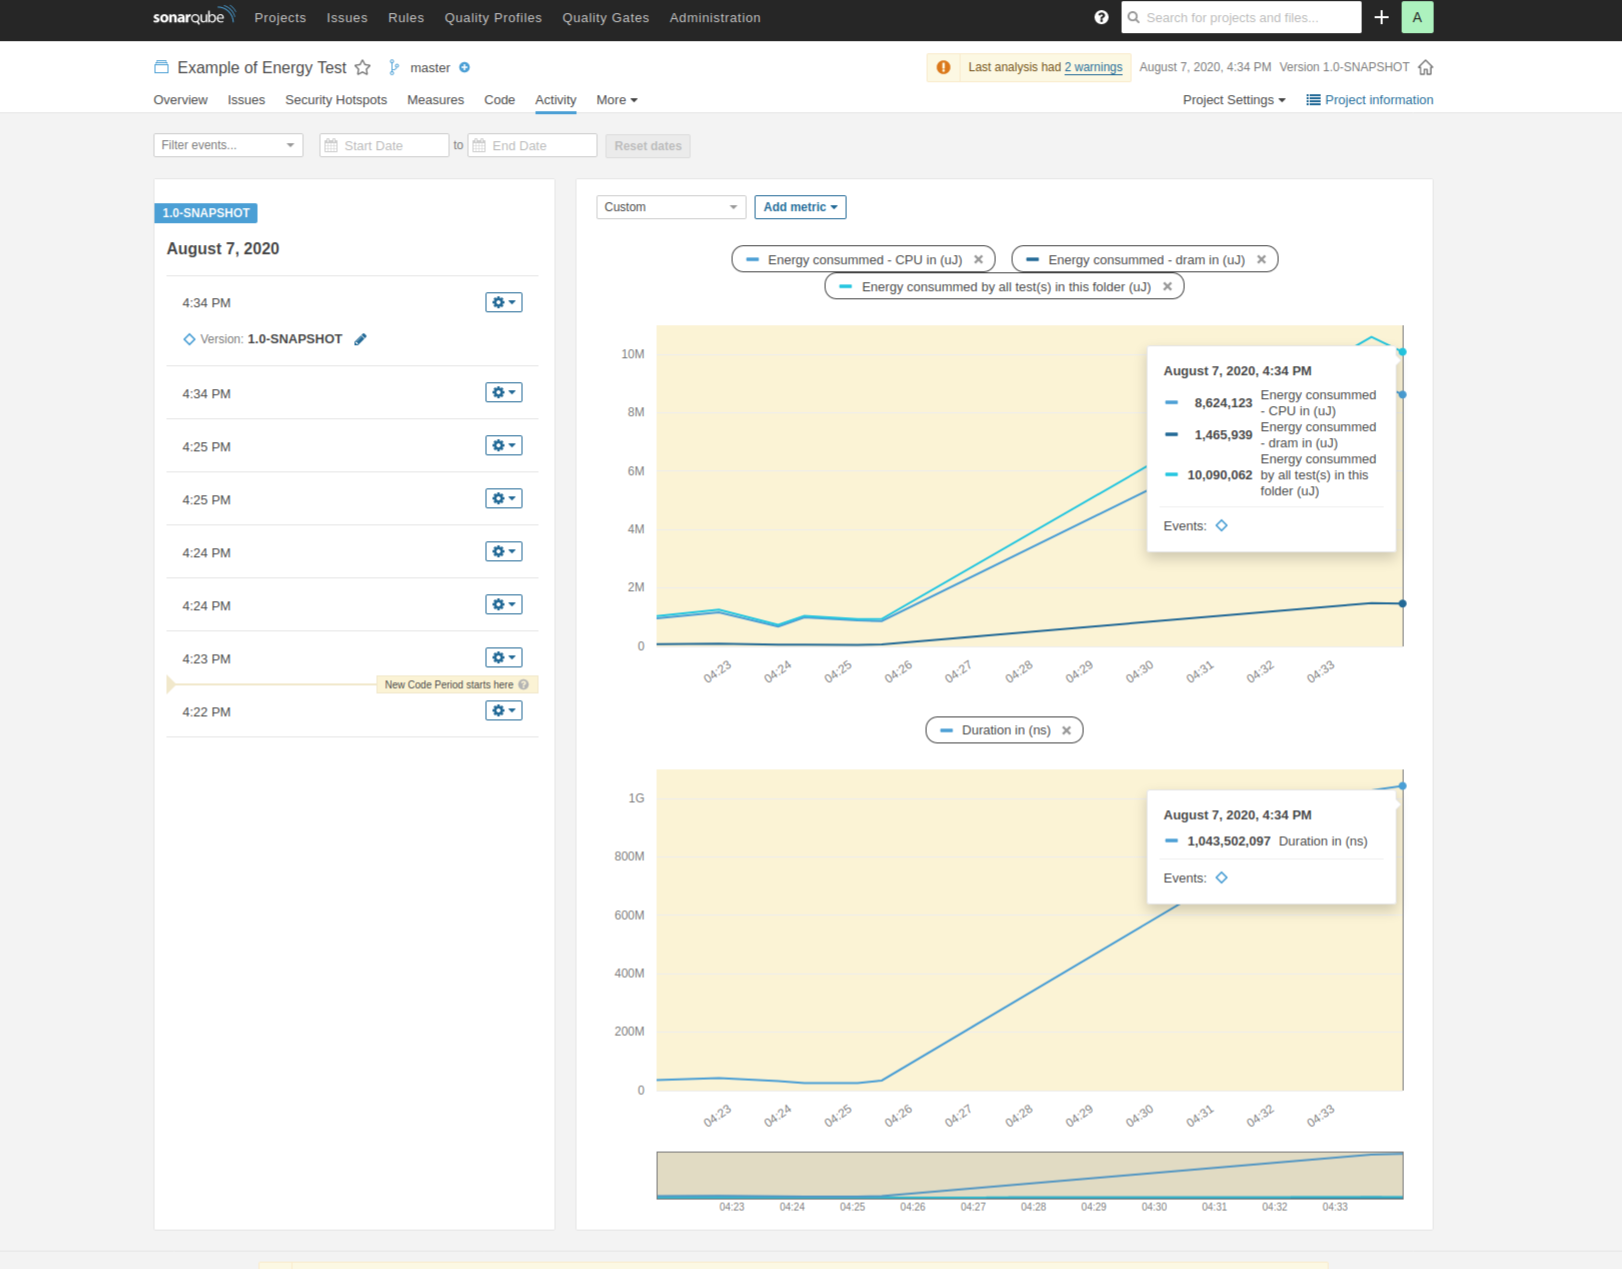
\includegraphics[width=0.8\linewidth]{chapters/JunitSonarplugin}
      \caption{Sonar plugin for Junit}
      \label{fig:JunitSonarplugin}
\end{figure}

we urge energy-efficiency benchmark developers to report measurements at nonpeak activity levels for a more complete characterization of a system's energy behavior\cite{barroso2007case}.


\subsubsection*{greenFaas}
servers operate most of the time at between 10 and 50 percent of their maximum utilization levels \cite{barroso2007case}


\begin{enumerate}

      \item lazy code, sacrificing the performance in order to get a better energy consumption --> green faas
      \item more representative benchmarks, using several CPU saturation levels
      \item measuring the energy impact instead of the row energy consumption. ( the highway analogy when a single application consumes less energy, however the total energy consumption of the system increases )
\end{enumerate}
\vfill \strut  % to fill the rest of the page with blank lines
\cleardoublepage
\begin{appendices}
\newpage
\addcontentsline{toc}{chapter}{APPENDICES}   

\chapter{Full Results:....}
\label{chapter:appendix_experimental_results_1}
\setcounter{table}{0}
\renewcommand{\thetable}{A.\arabic{table}}
\setcounter{figure}{0}
\renewcommand{\thefigure}{A.\arabic{figure}}

\newpage
\section*{Sequence 0}






\chapter{Full Results: ...}
\label{chapter:appendix_experimental_results_2}
\setcounter{table}{0}
\renewcommand{\thetable}{B.\arabic{table}}
\setcounter{figure}{0}
\renewcommand{\thefigure}{B.\arabic{figure}}
 
 
 
\newpage 
\section*{Sequence 0} 


 

\end{appendices} % Appendices

% ********************************** Back Matter *******************************
% Backmatter should be commented out, if you are usPing appendices after References
%\backmatter

% ********************************** Bibliography ******************************
\begin{spacing}{0.9}

  % To use the conventional natbib style referencing
  % Bibliography style previews: http://nodonn.tipido.net/bibstyle.php
  % Reference styles: http://sites.stat.psu.edu/~surajit/present/bib.htm

  \bibliographystyle{apalike}
  %\bibliographystyle{unsrt} % Use for unsorted references  
  %\bibliographystyle{plainnat} % use this to have URLs listed in References
  \cleardoublepage
  \bibliography{static_final_library} % Path to your References.bib file


  % If you would like to use BibLaTeX for your references, pass `custombib' as
  % an option in the document class. The location of 'reference.bib' should be
  % specified in the preamble.tex file in the custombib section.
  % Comment out the lines related to natbib above and uncomment the following line.

  %\printbibliography[heading=bibintoc, title={References}]


\end{spacing}

% ********************************** Appendices ********************************

% \begin{appendices} % Using appendices environment for more functunality

%     \include{Appendix1/appendix1}
%     \include{Appendix2/appendix2}

% \end{appendices}

% *************************************** Index ********************************
\printthesisindex % If index is present

\end{document}
